%\RequirePackage{pgfornament,tkzexample,tikzrput}  

\documentclass[a5paper,oneside]{amsart}
\usepackage[scale={.8,.85}]{geometry}
\usepackage{mathrsfs}
\usepackage[utf8]{inputenc}
\usepackage{dsfont}
\usepackage{listings}
\usepackage{color}\usepackage{mathtools}
\definecolor{azul}{RGB}{20,40,140}
\usepackage[colorlinks,linkcolor=azul, citecolor=azul,urlcolor=azul]{hyperref}
\usepackage{attachfile}
\usepackage{enumitem}
\setlength\parindent{0pt}

\mathtoolsset{showonlyrefs}
\newtheoremstyle{dotless}{}{}{\itshape}{}{\bfseries}{}{ }{}
\theoremstyle{definition}
\renewenvironment{proof}{{\bfseries Demostración:}}

\newtheorem{teorema}{\;\;Teorema}[section]
\newtheorem{problema}[teorema]{\;\;Problema}
\newtheorem{definicion}[teorema]{\;\;Definición}
\newtheorem*{categoria}{Categorías:}
\newtheorem*{remark}{Remark}
\setcounter{secnumdepth}{4}
\setcounter{tocdepth}{4}

%\setlength{\textwidth}{17.2cm} % was 18.2
%\setlength{\textheight}{23cm} % was 23
%\setlength{\topmargin}{-1cm} % was 0
%\setlength{\oddsidemargin}{-0.6cm}
%\setlength{\evensidemargin}{-0.6cm}

%\setlength{\textwidth}{18.9cm} % was 18.2
%\setlength{\textheight}{26.73cm} % was 23
%\setlength{\topmargin}{1cm} % was 0
%\setlength{\oddsidemargin}{0cm} %
%\setlength{\evensidemargin}{.8cm}
%% Arreglar pues ahora utilizas papel A4.

%Operadores

\DeclareMathOperator{\ivp}{IVP} %
\DeclareMathOperator{\sgn}{sgn} %
\DeclareMathOperator{\md}{mod}
\DeclareMathOperator{\ima}{Im}%
\DeclareMathOperator{\id}{Id} %
\DeclareMathOperator{\homo}{Hom} %
\DeclareMathOperator{\inter}{Int}
\DeclareMathOperator*{\Lim}{lim}
\DeclareMathOperator*{\Limsup}{lim\ sup}
\DeclareMathOperator*{\Liminf}{lim\ inf}
\DeclareMathOperator*{\Min}{m\text{\ii}n}
\DeclareMathOperator{\Aff}{Aff}
\DeclareMathOperator{\Affb}{\overline{\Aff}}
\DeclareMathOperator{\sdfd}{dfd}
\DeclareMathOperator{\scdfd}{dfd}
\DeclareMathOperator{\Beta}{B}
\DeclareMathOperator{\pd}{PD}
\DeclareMathOperator{\supp}{supp}
\DeclareMathOperator{\diam}{diam}
\newcommand{\ind}{\operatornamewithlimits{\perp}}
\DeclareMathOperator{\av}{Abs}
\DeclareMathOperator{\cb}{CB}
\DeclareMathOperator{\cbi}{CBI}
\DeclareMathOperator{\gwi}{GWI}
\DeclareMathOperator{\gw}{GW}
\newcommand{\rtree}{$\re$\nbd tree}
\newcommand{\leb}{\text{Leb}}
%Notaci?n



%Delimitadores
\newcommand{\ceil}[1]{\ensuremath{\lceil #1 \rceil}}
%\renewcommand{\floor}[1]{\ensuremath{\lfloor #1 \rfloor}}

%Formato
\newcommand{\defin}[1]{{\bf #1}}
\newcommand{\mc}[1]{\ensuremath{\mathscr{#1}}}
\newcommand{\bb}[1]{\mathbb{#1}}


%Notation

\newcommand{\card}[1]{\ensuremath{\left| #1 \right|}}
\newcommand{\lccb}{LCCB}
\newcommand{\pss}{S}
\newcommand{\compact}{K}
\newcommand{\psm}{\rho}
\newcommand{\ps}{\paren{\pss,\psm}}
\newcommand{\pse}{x}
\newcommand{\psep}{y}
\newcommand{\psepp}{z}
\newcommand{\saps}{\B_{\pss}}
\newcommand{\bre}{\B_{\re}}
\newcommand{\sko}{D}
\newcommand{\trees}{T}
\newcommand{\C}{C}
\newcommand{\refm}{\mu}
\newcommand{\den}{p}
\newcommand{\psd}[1]{\mc{P}_{#1}}
\newcommand{\s}{\ensuremath{\sigma}}
\newcommand{\bden}{M}
\newcommand{\hh}[1]{{\bf H#1}}
\newcommand{\ball}[2]{\imf{B_{#1}}{#2}}
\newcommand{\mmc}[1]{\imf{\tilde\omega}{#1}}
\newcommand{\rg}[1]{\ensuremath{\imf{\mathbb{G}}{#1}}}




\newcommand{\dfd}{\ensuremath{\stackrel{\sdfd}{=}}}
\newcommand{\deq}{\ensuremath{\stackrel{d}{=}}}

\newcommand{\ley}[2]{\ensuremath{\imf{\mc{L}^{#2}}{#1}}}
\newcommand{\leyc}[3]{\ensuremath{\imf{\mc{L}^{#3}}{#1\left|#2\right.}}}
\newcommand{\cond}[2]{\left.\vphantom{#2}#1\ \right| #2}

\newcommand{\e}{\ensuremath{\mathbf{e}}}
\newcommand{\esf}{\ensuremath{\mc{S}^{\downarrow}}}
%\newcommand{\ps}[1]{\mathscr{P}\paren{#1}}
\newcommand{\fun}[3]{\ensuremath{#1:#2\to #3}}
\newcommand{\fund}[3]{\ensuremath{#1:#2\mapsto #3}}
\newcommand{\set}[1]{\ensuremath{\left\{ #1\right\} }}
\newcommand{\sets}[1]{\ensuremath{{\mathbf #1}}}
\newcommand{\paren}[1]{\ensuremath{\left( #1\right) }}
\newcommand{\bra}[1]{\ensuremath{\left[ #1\right] }}
\newcommand{\seq}[1]{\ensuremath{ #1 _1,\ldots ,#1 _n }}
\newcommand{\sm}[3]{\left[ #1\right]_{#2}^{#3}}
\newcommand{\cde}{\Rightarrow}
\newcommand{\cdfd}{\ensuremath{\stackrel{\scdfd}{\cde}}}
\newcommand{\convo}[2]{\ensuremath{#2^{\!* #1}}}

\newcommand{\tl}[1]{\ensuremath{\hat{#1}}}

\newcommand{\matt}[3]{#1_{#2\, #3}}
\newcommand{\sip}{\bb{P}}
\newcommand{\jump}[2]{\ensuremath{\Delta #1_{#2}}}
\newcommand{\cadlag}{c\`adl\`ag}
\newcommand{\se}{\ensuremath{\bb{E}}}
\newcommand{\ssa}{\ensuremath{\mathscr{F}}}
\newcommand{\si}{{\ensuremath{\bf{1}}}}
\newcommand{\sbr}{\ensuremath{\mc{B}_{\re}}}
%\newcommand{\siind}{\ensuremath{\perp}}
\newcommand{\sigam}{\ensuremath{\Gamma}}
\newcommand{\smc}{\ensuremath{m}}
\newcommand{\sfleche}{S^{\downarrow}_f}

\newcommand{\gafun}[1]{\sigam \paren{#1}}
\newcommand{\poi}[1]{\ensuremath{\mc{P}\!_{#1}}}
\newcommand{\ber}[1]{\ensuremath{\mc{B}\!_{#1}}}
\newcommand{\fcpoi}[1]{\ensuremath{\hat{\mc{P}}\!_{#1}}}
%\newcommand{\ind}{\siind}
\newcommand{\condind}[3]{\ensuremath{#1\ind_{#3}#2}}
\newcommand{\sig}[1]{$\sigma$-\nobreakdash #1}
\newcommand{\sa}{\ensuremath{\sigma}\nbd field}
\newcommand{\realtree}{\ensuremath{\re}\nbd tree}
\newcommand{\eps}{\ensuremath{ \varepsilon}}
\newcommand{\na}{\ensuremath{\mathbb{N}}}
\newcommand{\en}{\ensuremath{\mathbb{Z}_+}}
\newcommand{\eti}{\ensuremath{\mc{U}}}
\newcommand{\etic}{\ensuremath{\mathbb{U}}}
\newcommand{\z}{\ensuremath{\mathbb{Z}}}
\newcommand{\re}{\ensuremath{\mathbb{R}}}
\newcommand{\ra}{\ensuremath{\mathbb{Q}}}
\newcommand{\com}{\ensuremath{\mathbb{C}}}
\newcommand{\con}[1]{\ensuremath{\overline{#1}}}
\newcommand{\proba}[1]{\ensuremath{\sip\! \left( #1 \right)}}
\newcommand{\probas}[2]{\ensuremath{#1\! \left( #2 \right)}}
\newcommand{\probac}[2]{\ensuremath{\sip\! \left( #1 \, | #2 \right)}}
\newcommand{\esp}[1]{\ensuremath{\se\! \left( #1 \right)}}
%\newcommand{\espc}[2]{\ensuremath{\se\! \left( #1 | #2 \right)}}
\newcommand{\espc}[2]{\ensuremath{\imf{\se}{\cond{#1}{#2}}}}
\newcommand{\var}[1]{\ensuremath{\text{Var}\! \left( #1 \right)}}
\newcommand{\cov}[1]{\ensuremath{Cov\! \left( #1 \right)}}
\newcommand{\abs}[1]{\hspace{.25mm}\left|#1\right|\hspace{.25mm}}
\newcommand{\ila}[2]{\ensuremath{\int #1\, d#2}}
\newcommand{\ilas}[3]{\ensuremath{\int_{#1} #2\, d#3}}
\newcommand{\il}[3]{\ensuremath{\int #1\, \imf{#2}{d#3}}}
\newcommand{\is}[4]{\ensuremath{\int_{#1} #2\, \imf{#3}{d#4}}}
\newcommand{\lp}[2]{\ensuremath{\mc{L}_#1\!\paren{#2} }}
\newcommand{\lpc}[4]{\ensuremath{\mc{L}_#1\!\paren{ #2 , #3 , #4 }}}
\newcommand{\ip}[1]{\ensuremath{\int #1\, d\sip }}
\newcommand{\ips}[2]{\ensuremath{\int_{#1} #2\, d\sip}}
\newcommand{\uF}{\ssa^u}
\newcommand{\G}{\ensuremath{\mc{G}}}
\newcommand{\h}{\ensuremath{\mc{H}}}
\newcommand{\B}{\ensuremath{\mc{B}}}
\newcommand{\f}[1]{\ssa_{#1}}
\newcommand{\fx}[2]{\ssa_{#1}^{#2}}
\newcommand{\indi}[1]{\si_{#1}}
\newcommand{\imi}[2]{#2^{-1}\!\paren{#1}}
\newcommand{\ooo}{\ensuremath{ \omega  } }
\newcommand{\oo}{\ensuremath{ \Omega  } }
\newcommand{\p}{\ensuremath{ \sip  } }
\newcommand{\q}{\ensuremath{ \bb{Q}  } }
\newcommand{\ofp}{\ensuremath{ \paren{ \Omega ,\F ,\p } } }
\newcommand{\med}[2]{\ensuremath{\paren{#1}{#2}}-medible}
\newcommand{\vat}{\ensuremath{\fun{X}{\oo}{\re}}\ }
\newcommand{\pix}[1]{\ensuremath{\sip}_{\! #1}}
\newcommand{\px}[2]{\ensuremath{\sip_{\! #1}\!\paren{#2}}}
\newcommand{\pxc}[3]{\ensuremath{\sip_{\! #1}\!\left( #2 | #3 \right)}  }
\newcommand{\br}{\sbr}
\newcommand{\sag}[1]{\sigma\!\paren{#1}}
\newcommand{\cs}[1]{\ensuremath{#1}-p.s.}
\newcommand{\ore}{ \ensuremath{\overline{\re}}}
\newcommand{\fungen}[1]{\ensuremath{\varphi_{#1}}}%Comando para la notaci�n de funci�n generadora.
\newcommand{\cbin}[2]{\ensuremath{\paren{\begin{array}{c}#1\\#2\end{array}}}}
\newcommand{\fa}[2]{\ensuremath{{#1}^{\paren{#2}}}}
\newcommand{\dnor}[2]{\ensuremath{N(#1,#2)}}
\newcommand{\mb}{movimiento browniano}
\newcommand{\moc}[3]{\smc^{#3}(#1,#2)}
\newcommand{\clo}[1]{\ensuremath{\overline{#1}}}
\newcommand{\inte}[1]{\ensuremath{\inter #1}}
\newcommand{\fro}[1]{\ensuremath{\partial\paren{ #1}}}
\newcommand{\cd}[2]{\ensuremath{#1\stackrel{\mc{D}}{\to}#2}}
\newcommand{\pr}[3]{\ensuremath{#1_{#2}\!\paren{#3}}}
\newcommand{\oi}[1]{\ensuremath{\mc{O}\paren{#1}}}
\newcommand{\mw}{\ensuremath{\mathbb{P}}}
\newcommand{\me}{\ensuremath{\pi}}


\newcommand{\nbd}{\nobreakdash -}
\newcommand{\ii}{\'{\i}}
\newcommand{\n}{\~n}
\newcommand{\imf}[2]{\ensuremath{#1\!\paren{#2}}}
\newcommand{\floor}[1]{\ensuremath{\lfloor #1\rfloor}}
\newcommand{\proint}[2]{\ensuremath{\langle #1,#2\rangle}}
\newcommand{\vp}{\ensuremath{\varphi}}
\newcommand{\noru}[1]{\ensuremath{\|#1\|}}
\newcommand{\gen}[1]{\ensuremath{|#1 |}}
\newcommand{\vc}[1]{\ensuremath{\langle #1\rangle}}
\newcommand{\pc}[2]{\ensuremath{\langle#1,#2\rangle}}
\newcommand{\vcd}[1]{\ensuremath{\left[#1\right]}}

\newcommand{\sml}{\ensuremath{\nu}}
\newcommand{\ml}[1]{\ensuremath{\imf{\sml}{#1}}}
\newcommand{\va}[2]{\ensuremath{\imf{V_{#1}}{#2}}}
\newcommand{\clase}[1]{\ensuremath{\mc{C}^{#1}}}
\newcommand{\marte}[2]{\ensuremath{\imf{\mc{E}^{#2}}{#1}}}

\newcommand{\dencero}[1]{\ensuremath{\left. \frac{\partial }{\partial #1}\right|_{#1=0} }}
%\newcommand{\premin}[1]{\ensuremath{\stackrel{\leftarrow}{#1}}}
%\newcommand{\postmin}[1]{\ensuremath{\stackrel{\rightarrow}{#1}}}
\newcommand{\premin}[1]{\ensuremath{{#1}^{\leftarrow}}}
\newcommand{\postmin}[1]{\ensuremath{{#1}^{\rightarrow}}}



%Ambientes (Environments)

\newenvironment{esn}{\begin{equation*}}{\end{equation*}}
\newenvironment{ecn}{\begin{equation}}{\end{equation}}
\newenvironment{listeo}{\begin{list}{\alph{enumi})}{\usecounter{enumi}}}{\end{list}}
\newenvironment{numerai}{\begin{list}{\roman{enumi})}{\usecounter{enumi}}}{\end{list}}
\newcommand{\N}{\mathbb{N}}
\newcommand{\R}{\mathbb{R}}
\newcommand{\E}{\mathbb{E}}

\newcommand{\F}{\mathscr{F}}

\newcommand{\indic}{\mathds{1}}

\newcommand{\textme}[1]{\;\text{#1}\;}
\newcommand{\nqed}{
	\null
	\null
	\null
	\null	
	\center{
		\textbf{---------------------------------------------------------------------------------------}
	}
	\newpage
}



\numberwithin{section}{part}
\numberwithin{equation}{subsection}


%\renewcommand{\nqed}
{		
		\null
		\null
		\null
		\null
		\begin{tikzpicture}
			\node (A) at (0,0) {};
			\node (B) at (3,0) {};
			\node (C) at (6,0) {};
			\path (A.center) to [ornament=86,at=0] (B.center);
			\path (A.center) to [ornament=85,at=0.50] (B.center);
			\path (A.center) to [ornament=88,at=0.75] (C.center);
    		\path (B.center) to [ornament=85,at=1.50] (C.center);
			\path (B.center) to [ornament=86,at=2] (C.center);
		\end{tikzpicture}\\
		\newpage
}




\title[Problemas de Procesos I]{
    Problemas de Procesos Estocásticos I\\ 
    Semestre 2013-II\\ 
    Posgrado en Ciencias Matemáticas\\ 
    Universidad Nacional Autónoma de México\\
    Héctor Manuel Téllez Gómez
}

\begin{document}
    \maketitle
    \part{Tarea 1}
        \subsection{Problema 1.1}
\begin{problema}
	Sea $\left({X_n}_{n\in\mathbb{N}}\right)$ un proceso estocástico con valores reales y $A\subset \mathbb{R}$ un boreliano. 
	Pruebe que si
	\begin{align}
		T_0=0\quad\text{y}\quad T_{n+1}=\min\{k>T_n: X_k\in A \subset \mathbb{R}\}
	\end{align}
	entonces $T_n$ es un tiempo de paro para toda $n$ y $T_n\to \infty$ puntualmente conforme $n\to\infty$. 

	\begin{categoria} 
		Tiempos de paro.
	\end{categoria}
\end{problema}
		
\begin{proof}
\\

	Sea $(\mathscr{F}_n = \sigma(  X_0, X_1, \dots, X_n ))_{ n \in \mathbb{N}}$ una filtración.
\\

	Veamos que $T_0$ es tiempo de paro. $\{T_0 = 0\} = \Omega \in \mathscr{F}_n$ y 
	$\{T_0 = c\} = \emptyset \in \mathscr{F}_n$ para $c \not= 0 \in \mathbb{N}$. Recordemos que:		
	\begin{align}\label{problema_1_1:equivalencia_varable_aleatoria}
		\{T_0 = n\} \in \mathscr{F}_n \; \forall n \in \mathbb{N} \iff 
		\{T_0 \leq n\} \in \mathscr{F}_n \; \forall n \in \mathbb{N}.
	\end{align}
	Y por lo tanto $T_0$ es variable aleatoria sobre la sigma álgebra $\sigma(\cup_{n \in \mathbb{N}} 
	\mathscr{F}_n)$.

	Para $n=1$, veamos que:
 
	\begin{align}
			\{T_1 = 1\}     &= \{ X_1 \in A \}	\in \mathscr{F}_1 
	\end{align}
	
	\begin{align}
			\{T_1 = 2\} 	&= 	\{ X_1 \not\in A, X_2 \in A \} \\
							&= 	\{ X_1 \not\in A \} \cap \{X_2 \in A \} \in \mathscr{F}_2	
	\end{align}
	
	\begin{align}
			\{T_1 = 3\} 	&=	\{ X_1 \not\in A, X_2 \not\in A,  X_3 \in A \} \\ 
							&= 	\{ X_1 \not\in A \} \cap \{ X_2 \not\in A \} \cap \{X_3 \in A \} \in \mathscr{F}_3
	\end{align}
	
	\begin{align*}
		\vdots
	\end{align*}
	
	\begin{align}
			\{T_1 = n\} 	&=	\{ X_1 \not\in A, X_2 \not\in A, \dots, X_{n-1} \not\in A, X_n \in A \} \\
							&= 	\bigcap_{i=1}^{i=n-1} \{ X_i \not\in A \} \cap \{X_n \in A \} \in \mathscr{F}_n
	\end{align} 
 
	Por hipótesis de inducción supongamos que $\{T_k = n\} \in \mathscr{F}_n$ para cierta $k>1$ 
	y para toda $n \in \mathbb{N}$ . \\

	Para demostrar la primera parte del ejercicio, basta probar que $\{T_{k+1} = n\} \in \mathscr{F}_n$ para 
	toda $n \in \mathbb{N}$. Pues por lo dicho en (\ref{problema_1_1:equivalencia_varable_aleatoria}) resultarían ser 
	variables aleatorias en $\sigma(\cup_{n \in \mathbb{N}} \mathscr{F}_n)$.
	\\
	
	Dado que 
	\begin{align}\label{problema_1_1:T_n->infty}
		0=T_0<T_1<T_2<\dots<T_k
	\end{align}  
	tenemos que $\{ T_k = n\} = \emptyset \in \mathscr{F}_l$ para $n < k$. 
	
	Ahora, sea $n \geq k$
	
	\begin{align}\label{problema_1_1:T_k+1}
		\{ T_{k+1} = n\} = 
		\left( \bigcup_{i < n } \{T_k = i \} \right) 
		\cap 
		\left( \bigcap_{i < n} \{ X_i \not\in A \} \right)
		\cap
		\{ X_n \in A\}
	\end{align}
	
	
	Donde 
	\begin{itemize}
		\item	 $\{ T_k = i\} \in \mathscr{F}_n \; \forall i < n \in \mathbb{N} \; $ (Por hipótesis de inducción).	
		\item	 $\{ X_i \not \in A\} \in \mathscr{F}_n \; \forall i < n \in \mathbb{N} \;$ (Por ser $\mathscr{F}$ filtración).
		\item $\{ X_n \in A\} \in \mathscr{F}_n$ (Por ser $X_n$ variable aleatoria en $\mathscr{F}_n$)	
	\end{itemize}
	
	Y por lo tanto, (\ref{problema_1_1:T_k+1}) pertenece a $\mathscr{F}_n$. Con lo que termina la demostración de la primera parte del ejercicio.\\
	
	Ahora, de (\ref{problema_1_1:T_n->infty}) se sigue inmediatamente que que $T_n \rightarrow \infty$.
\end{proof}
\newpage

\subsection{Problema 1.2}
\begin{problema}
		Suponga que \(T\) es un tiempo de paro tal que para algún 
		\(N\in\mathbb{N}\) y \(\varepsilon>0\) se tiene que para toda \(n\in\mathbb{N}\):
		\begin{equation}\label{problema1_2:hipotesis_del_problema}
		\mathbb{P} (T \leq N + n | F_n) > \varepsilon \text{ casi seguramente}
		\end{equation}
		Al verificar la desomposici\'on
		\begin{equation}\label{problema1_2:sugerencia_del_problema}
			\mathbb{P} (T>kN)= \mathbb{P} (T>kN,T>(k-1)N)
		\end{equation}
		pruebe por inducci\'on que para cada \(k=1,2,\ldots\):
		\begin{align}
			\mw(T>kN)\leq (1-\varepsilon)^k.
		\end{align}
		Pruebe que \( \mathbb{E}(T)<\infty \). 
	\begin{categoria} Tiempos de paro.\end{categoria}
\end{problema}

\begin{proof}
	Tenemos que: 
	
	\begin{align}
		(T>kN \Rightarrow T>(k-1)N 	&\Rightarrow (T>kN) \subset (T>(k-1)N) \\ 
									&\Rightarrow (T>kN) \cap (T>(k-1)N) = (T>kN) \\ 
									&\Rightarrow \mw(T>kN, T>(k-1)N) = \mw(T>kN)	
	\end{align}
		
	\textbf{Base de inducción.} $k=1$. Usando \eqref{problema1_2:hipotesis_del_problema}, con $n=0$ 
	\begin{align}
		\mw(T\leq 1N | \F_0) > \epsilon\Rightarrow
		\mw(T>N| \F_0) < 1 - \epsilon
	\end{align}
	Sustituyendo por la definición de probabilidad condicional tenemos:
		\begin{align}
			\E(\indic_{T>N} | \F_0)	&= \mw(T>N| \F_0) 
									&< 1 - \epsilon
		\end{align}
	Aplicando esperanza en ambos lados tenemos:
		\begin{align} 
			\mw(T>N) 	&= 	\E(\E(\indic_{T>N} | \F_0)) 
						&< 	\E(1 - \epsilon) 
						&= 1 - \epsilon.
		\end{align}
	
	\textbf{Hipótesis de induccion.} Supongamos que $\mw(T>k_0N)\leq(1 - \epsilon)^{k_0}$ para algún $k_0 \geq 1$.
	
	\textbf{Paso inductivo.} 
	Utilizando \eqref{problema1_2:sugerencia_del_problema} tenemos que
		\begin{align}
			\mw(T>(k_0+1)N) = \mw(T>(k_0+1)N, T>k_0N) = \E(\indic_{T>(k_0+1)N} \cdot \indic_{T>k_0N}).
		\end{align}
	Ahora, dado que $T>k_0N$ es un conjunto $\F_{k_0N}$-medible tenemos:
	\begin{align} 
		\E(\indic_{T>(k_0+1)N} \cdot \indic_{T>k_0N}) 	&=		\E\left(\E\left(\indic_{T>(k_0+1)N} \cdot \indic_{T>k_0N} | \F_{k_0N}\right)\right) \\ 
														&=		\E\left(\indic_{T>k_0N} \E\left(\indic_{T>(k_0+1)N}|\F_{k_0N}\right)\right) \label{problema1_2:resultado_preliminar}
	\end{align}
	Utilizando  $n=k_0N$ en \eqref{problema1_2:hipotesis_del_problema} tenemos
	\begin{align}
		\mw\left(T>k_0N+N|\F_{k_0N}\right) = \E\left(\indic_{T>(k_0+1)N}|\F_{k_0N}\right) < 1-\epsilon
	\end{align}
	Sustituyendo esto último en \eqref{problema1_2:resultado_preliminar} obtenemos:
		\begin{align}
				 E\left(\indic_{T>k_0N} \E\left(\indic_{T>(k_0+1)N}|\F_{k_0N}\right)\right) 	&< 		E\left(\indic_{T>k_0N} (1-\epsilon)\right) \\
																								&=	 	(1-\epsilon) E\left(\indic_{T>k_0N} \right) \\
																								&=		(1-\epsilon) \mw(T>k_0N) \\
																								&\leq   (1-\epsilon)(1-\epsilon)^{k_0} \\
																								&= (1-\epsilon)^{k_0 + 1}.
		\end{align}
	Con lo que concluimos
		\begin{align}
			\mw(T>(k_0+1)N) &\leq (1-\epsilon)^{k_0 + 1}.
		\end{align}
	Terminando así la demostración por inducción.\\
	
	
	Para la siguiente prueba notemos que si $X$ es una variable aleatoria y $r > s \in \mathbb{R}$ entonces
	$(X > s) \subset (X > r)$ y por lo tanto $\mw(X > s) \leq \mw(X > r)$.\\
	
	En particular para nuestro tiempo de paro $T$, si dado $n \in \mathbb{N}$, $k \in \mathbb{N}$ es tal que 
	$kN \geq n < (k+1)N$, entonces $\mw(T > n) \leq \mw(T > kN)$.\\	

	Trabajando por bloques de tamaño $N$ tenemos que 
	\begin{align}
		\sum_{n = kN}^{(k+1)N -1} \mw(T > n) \leq N \mw(T > kN).
	\end{align}		
	
	También recordemos que si $T$ es una variable aleatoria positiva con valores en los enteros entonces 
	\begin{align}
		\E(T) = \sum_{n=0}^{\infty} \mw(T > n).
	\end{align}
	
	Sustituyendo nuestro penúltimo razonamiento en esta ultima fórmula tenemos:
	
	\begin{align}
		\E(T) 	&= 		\sum_{n=0}^{\infty} \mw(T > n) \\
				&= 		\sum_{k=0}^{\infty} \sum_{n = kN}^{(k+1)N -1} \mw(T > n) \\
				&\leq 	N \sum_{k=0}^{\infty} \mw(T > kN)
	\end{align}
		
	Sustituyendo nuetstro resultado de que $\mw(T>kN)<(1-\epsilon)^{k}$ resulta que:
	\begin{align}
		\E(T)\leq N \sum_{k=0}^{\infty} \mw(T > kN) \leq N \sum_{k=0}^{\infty} (1-\epsilon)^k.
	\end{align}
	
	De lado derecho de esta última desigualdad tenemos una serie geométrica. Dado que $\epsilon$ es mayor 
	que $0$ y entonces que $1-\epsilon$ es menor que $1$, tenemos que es una serie geométrica que converge 
	en los reales y por lo tanto $\E(T)$ está acotada por un número real.
	
\end{proof}	
\newpage

\subsection{Problema 1.3}
\begin{problema}
	\emph{Tomado de Mathematical Tripos, Part III, Paper 33, 2012, \url{http://www.maths.cam.ac.uk/postgrad/mathiii/pastpapers/}}

	Sean $\paren{X_i,i\in\na}$ variables aleatorias 
	independientes con $\proba{X_i=\pm 1}=1/2$. Sean $S_0=0$ y $S_n=\sum_{i=1}^n X_i$. 

	\begin{enumerate}
		\item[(i)] Sea $T_1=\min\set{n\geq 0:S_n=1}$. Explique por qu\'e $T_1$ es un 
		tiempo de paro y calcule su esperanza.
		
		\item[(ii)] Mediante el inciso anterior, construya una martingala que converge 
		casi seguramente pero no lo hace en $L_1$.
		
		\item[(iii)] Sea $M_n$ la martingala obtenida al detener a $-S$ en $T_1$. Utilice la solución al
		Problema de la Ruina para probar que $\mw(max_n M_n \geq M) = 1/(M+1)$ para todo $M \geq 1$. Concluya que
		$\E(max_m M_n) = \infty$ y que por lo tanto $\E(max_{m\leq n} M_m) \rightarrow \infty$ conforme 
		$n \rightarrow \infty$. Finalmente, deduzca que no puede haber una desigualdad de tipo Doob cuando $p=1$.
		
		\item[(iv)] Sea $T=\min\set{n\geq 2:S_n=S_{n-2} + 2}$ y $U=T-2$. ?`Son $T$ y $U$ 
		tiempos de paro? Justifique su respuesta.
		
		\item[inciso (v)] Para la variable $T$ que hemos definido, calcule $\esp{T}$. 
	\end{enumerate}

	\defin{Categor\'ias: } Tiempos de paro, problema de la ruina
\end{problema}
\begin{proof}
	\subsubsection{Inciso (i)}
	\emph
{
	Sea $T_1=\min\set{n\geq 0:S_n=1}$. Explique por qu\'e $T_1$ es un 
	tiempo de paro y calcule su esperanza.
}

\afterstatement\pn

	Consideremos a la filtración $(\F_n)_{n\in\N}$ como la filtración 
	generada por $X_1, X_2, \dots$.\pn

	Es decir, $F_0 = \{\emptyset, \Omega\}$, $\F_n = \sigma(X_1, X_2, \dots, X_n)$\pn

	Nótese que $S_0$ es medible bajo cualquier sigma álgebra por ser constante, en particular bajo
	$\F_0$.\pn

	Basta demostrar que $(T_1 = n) \in \F_n$ para ver que $T_1$ es tiempo de paro. $T_1$ 
	representa el primer tiempo en que la suma es igual a $1$. Es decir, para cualquier 
	momento anterior, la suma no es $1$.\pn

	Eso escrito en símbolos significa:

    \begin{align}
        (T_1 = n) = \bigcap_{i=0}^{n-1}(S_i \not= 1) \cup (S_n = 1).
    \end{align}\pn

	Para $n=0$, $(S_0 = 1) = \omega \in \F_0$.\pn

	Como $(S_i \not= 1) \in \F_j$ siempre que $i \leq j$. Para $n>0$, $(T_1 = n)$ es el resultado de 
	unir e intersectar conjuntos $\F_n$-medibles, lo cual resulta $\F_n$-medible.\pn

	Para $m \in \N$. Definamos $T_m = min\{n \geq 0 : S_n = m\}$ 
	(Nótese que para el caso $m=1$, esta definición	coincide con la definición previa de $T_1$).\pn
	
	Para $a,b \in \N$, podemos definir el tiempo de paro $T_{a,b} = T_{-a} \wedge T_b$, y 
	corresponde al 	tiempo de paro del problema de la ruina. Para este tiempo de paro ya conocemos 
	la esperanza y es
	
    \begin{align}
        \E(T_{a,b}) = ab.
    \end{align}\pn
	
	Ahora, tomemos la sucesion de variables aleatorias
    
    \begin{align}
        T_{1,1}, T_{2,1}, T_{3,1}, \dots, T_{n,1},\dots
    \end{align}\pn 
    
    Notemos que si $a>a' \in N$ entonces $T_{-a} > T_{-a'}$, pues $T_{-a}$ es la primera vez
	que se llega a $-a$, y para poder alcanzar $-a$ era necesario haber pasado por $-a'$.
	De aqui tenemos que si $a>a'$, entonces $T_{a,1} \geq T_{a',1}$. De donde nuestra sucesión es 
	no decreciente.\pn
	
	Por otro lado, que si $a>a' \in N$ entonces $T_{-a} > T_{-a'}$ implica que $T_{-n} n \in \N$ es 
	una sucesión extrictamente creciente y por lo tanto 
	$\lim\limits_{n \rightarrow \infty} T_{-n} = \infty$, con esto tenemos que el límite de nuestra 
	sucesión es 
	
    \begin{align}		
        \lim_{n\rightarrow\infty} T_{n,1}   &=  \lim_{n\rightarrow\infty} T_{-n} \wedge T_1 \\
                                            &=  \infty \wedge T_1                           \\
                                            &=  T_1
	\end{align}\pn

	Tenemos todos los ingredientes para usar Teorema de convergencia monótona sobre nuestra sucesión
	y la variable $T_1$. Nuestra sucesion es monótona y converge puntualmente a $T_1$. Utilizando
	dicho teorema obtenemos:
	
	\begin{align}
        \E(T_1)     &=  \E(\lim_{n\rightarrow\infty} T_{n,1})       \\
                    &=  \lim_{n\rightarrow\infty} \E(T_{n,1})       \\
                    &=  \lim_{n\rightarrow\infty} n\cdot 1          \\
                    &=  \infty.
	\end{align}\pn
	
	Lo cual era intuitivo. Si $\E(T_1)$ fuese finito, diría que existe un número de volados donde
	uno puede apostar con mucha certeza que ganará un peso después de jugar "cerca" de esa cantidad
	de volados. Intuitivamente, esto vuelve injusto un juego de volados donde la moneda es
	justa.	
	\newpage
	
	\subsubsection{Inciso (ii)}
	\emph
{	
	Mediante el inciso anterior, construya una martingala que converge 
	casi seguramente pero no lo hace en $L_1$.\\
}
\afterstatement	
	En [\ref{problema1_4}] se probará que si $T$ y $S$ son tiempos de paro, entonces $T\wedge S$ también 
	es tiempo de paro. Con esto tenemos que si $T_1$ es tiempo de paro, entonces $T_1 \wedge n$ con 
	$n \in \N$ también es tiempo de paro. Definimos entonces 
	$$M_n = S_{T_1 \wedge n}.$$
	
	Veamos que los $M_n$ forman una martingala.
	
	\begin{itemize}
		\item 
			$M_n$ es adaptada a la filtración.
			\begin{align}
				M_n(w) = S_{T_1 \wedge n}(w) = 
				S_{T_1 \wedge n (w)}(w) = 
				\sum_{k=1}^{T_1 \wedge n (w)} X_k = 
				\sum_{k=1}^{n} (X_k \cdot \indic_{T_1 \geq k})(w).
			\end{align}
			
			De donde, podemos escribir:
			\begin{align}\label{problema1_3:descomposicion_de_M_n}
				M_n = \sum_{k=1}^{n} (X_k \cdot \indic_{T_1 \geq k}).
			\end{align}\pn							 		
			
			Recordemos que $X_k$ es $\F_n$-medible para toda $k \leq n $. Por ser
			$T_1$ tiempo de paro, los conjuntos $A_k = \{T_1 = k\}$ y 
			$B_k = \{T_1 \leq k\}$	son $F_k$ medibles y por lo tanto 
			$A_k \cup B_k^c = \{ T_1 \geq k\}$ también lo es. De aquí que 
			$\indic_{T_1 \geq k}$ es $\F_k$-medible y por lo tanto también $\F_n$-medible
			para toda $n$ tal que $n \geq k$.\pn
			  
			Entonces $M_n$ es suma y productos de funciones $\F_n$-medibles y por lo tanto
			$F_n$-medible. Que es lo que queríamos demostrar.\pn
			
		\item
			$M_n \in L_1$\pn
			
			De \eqref{problema1_3:descomposicion_de_M_n} podemos ver que $M_n$ es 
			suma finita de variables acotadas. Por lo tanto $M_n \in L_1$.\pn
			
		\item Ahora probaremos que	$\E(M_{n+1} | \F_{n}) = M_{n}$\pn
			
			Primero:
			\begin{align}
				\E(M_{n+1} | \F_{n})    &=  \E( S_{T_1 \wedge (n+1)} | \F_{n})                                                          \\
                                        &=  \E\bigg( \sum_{k=1}^{n+1} (X_k \cdot \indic_{T_1 \geq k})\bigg| \F_{n}\bigg)                \\	 			
                                        &=  \E\bigg( \sum_{k=1}^{n} (X_k \cdot \indic_{T_1 \geq k}) \bigg| \F_{n}\bigg) +
                                            \E\bigg((X_{n+1} \cdot \indic_{T_1 \geq n+1}) \bigg| \F_{n}\bigg)                           \\
                                        &\comment{Este paso es gracias a que $X_k$ y $\indic_{T_1 \geq k}$ son $\F_n$-medibles}  		\\
                                        &=  \sum_{k=1}^{n} (X_k \cdot \indic_{T_1 \geq k}) + 
                                            \E((X_{n+1} \cdot \indic_{T_1 \geq n+1}) | \F_{n})                                          \\
                                        &=  S_{T_1 \wedge n} + \E((X_{n+1} \cdot \indic_{T_1 \geq n+1}) | \F_{n})                       \\
                                        &=  M_n + \E((X_{n+1} \cdot \indic_{T_1 \geq n+1}) | \F_{n})
			\end{align}
			
			Entonces, nos basta probar que $\E(X_{n+1} \cdot \indic_{T_1 \geq n+1} |
			 \F_{n}) = 0$ para terminar nuestra demostración.\pn
			 
			Sean $A = \{T_1 = n\}$ y $B = \{ T_1 \leq n\}$. Por ser $T_1$ tiempo de paro,
			$A$ y $B$ son $\F_n$-medibles. Por lo tanto $B \setminus A$ también es $\F_n$-medible. 
			Notemos que $\{T_1 \geq n+1\} = (B \setminus A)^c$. Por lo tanto $\{T_1 \geq n+1\}$ es
			$\F_n$-medible. De donde  $\indic_{T_1 \geq n+1})$ es $\F_n$-medible.\pn
			
			Con esto, ahora tenemos que:
			\begin{align}
				\E((X_{n+1} \cdot \indic_{T_1 \geq n+1}) | \F_{n})  &=  \indic_{T_1 \geq n+1} \cdot \E(X_{n+1} | \F_{n})                        \\
                                                                    &\;\;\;\;\mbox{(Este paso es gracias a que los }                            \\
                                                                    &\;\;\;\;\;\mbox{$X_n$ son independientes)}                                 \\
                                                                    &=  \indic_{T_1 \geq n+1} \cdot \E(X_{n+1} )                                \\
                                                                    &=  \indic_{T_1 \geq n+1} \cdot 0                                           \\
                                                                    &=  0
			\end{align}\pn
			
			Como queríamos demostrar.
	\end{itemize}
	
	Ahora que tenemos que $(M_n)_{n \in \N}$ es martingala, confirmemos que converge casi seguramente.\pn
	
	Notemos que $(T_1 \wedge n)_{n \rightarrow \infty} \rightarrow T_1$ c.s.\pn
	
	De aquí que $(M_n)_{n \rightarrow \infty} = (S_{T_1 \wedge n})_{n \rightarrow \infty} = S_{T_1}$ c.s.\pn				
	
	Veamos que la convergencia no ocurre en $L_1$.\pn
				
	Dado que $T_1 \wedge n$ es un tiempo de paro acotado para toda $n \in \N$,
	podemos aplicar el Teorema de Muestreo Opcional de 	Doob. 
	El cual nos dice que $\E(M_n) = \E(S_{T_1 \wedge n}) = \E(S_0) = 0$.\pn
	
	Por otro lado, por definición de $T_1$, $S_{T_1} = 1$ c.s.	De donde $\E(S_{T_1}) = 1$.
	
	\begin{align}
		\E(M_n) = 0 \not\rightarrow 1 = \E(S_{T_1}).
	\end{align}\pn			
	
	Y con esto, queda demostrado que la convergencia no se da en $L_1$.	
	\newpage
	
	\subsubsection{Inciso (iii)}
	\emph{
	Sea $M_n$ la martingala obtenida al detener a $-S$ en $T_1$. Utilice la solución al
	Problema de la Ruina para probar que \\
	$\mw(max_n M_n \geq M) = 1/(M+1)$ para todo $M \geq 1$. Concluya que\\
	$\E(max_m M_n) = \infty$ y que por lo tanto $\E(max_{m\leq n} M_m) \rightarrow \infty$ conforme 
	$n \rightarrow \infty$. Finalmente, deduzca que no puede haber una desigualdad de tipo Doob cuando $p=1$.
}\pn
	
\afterstatement

	Definimos $M_n = -S_{T_1 \wedge n}$. Notemos que $M_n$ únicamente toma valores en $[-1, \infty]$.
	Para calcular $\mw(max_n M_n \geq M)$ notemos primero que:

	\begin{align}
		\mw(max_n M_n \geq M) = 1 - \mw(max_n M_n < M).
	\end{align}\pn
	
	$\max_n M_n < M$ significa que $M_n$ nunca alcanza el valor $M$.\pn
	 
	Intentando hacer analogía con el problema de la ruina, pensemos en dos concursantes,
	uno con $1$ peso y otro con $M$ pesos. Nunca alcanzar $M$ significa que nunca gana el que tiene $1$ peso.\pn
	
	Esta probabilidad ya la conocemos y es 
	
	\begin{align}
		\mw(max_n M_n < M) = \frac{M}{M + 1}
	\end{align}\pn
		
	Por lo tanto
	
	\begin{align}
		\mw(max_n M_n \geq M) 	&= 1 - \mw(max_n M_n < M) \\
								&= 1 - \frac{M}{M + 1}\\
								&= \frac{M+1}{M+1} - \frac{M}{M + 1}\\
								&= \frac{1}{M+1}
	\end{align}\pn
	
	Utilizando este resultado:

	\begin{align} \label{problema1_3:esperanza_del_maximo_de_M_n}
		\E(max_n M_n) 	&= - \mw(max_n M_n = -1) + \sum_{M=1}^{\infty} \mw(max_n M_n \geq M) \\
						&= - \mw(max_n M_n = -1) + \sum_{M=1}^{\infty} \frac{1}{M+1} \\ 
						&= - \mw(max_n M_n = -1) + \infty \\
						&= \infty
	\end{align}\pn						
	
	Ahora, tenemos que:
    
	\begin{align}
		\|\overline{M_{n}^{+}}\|_1  &=    \E\left({\overline{M_{n}^{+}}}\right)     \\
									&=    \E\left({\max_{m \leq n}M_m^+}\right)     \\
									&\geq \E\left({\max_{m \leq n}M_m}\right)										
	\end{align}\pn
		
	Donde, el último término, tiende a infinito en base al resultado 
	\eqref{problema1_3:esperanza_del_maximo_de_M_n}.\pn

	Por otro lado:
    
	\begin{align}
		\|M_n^+\|_1=\|-S_{T_{1\wedge n}}^{+}\|_1  \longrightarrow  \|-S_{T_1}^+\|_1 = 0 < \infty
	\end{align}\pn
	
	Por lo tanto, no existe número $K$, tal que
	
    \begin{align}
		 \|\overline{M_n^+}\|_1 \leq  K \|M_n^+\|_1
	\end{align}\pn
	
	En otras palabras, no tenemos una desigualdad de tipo Doob para $p=1$.		
	\newpage
	
	\subsubsection{Inciso (iv)}
	\emph
{
	Sea $T=\min\set{n\geq 2:S_n=S_{n-2} + 2}$ y $U=T-2$. ?`Son $T$ y $U$ 
	tiempos de paro? Justifique su respuesta.
}\par\null

\afterstatement

	Intuitivamente, $T$ significa, el primer tiempo tal que ganamos en dos volados consecutivos.
	También intuitivamente, esto debería ser un tiempo de paro.\par\null
	
	Veamos que efectivamente así ocurre. Utilizando la siguiente prueba por inducción:\par\null
	
	\textbf{Base de inducción:}\par\null		
    
		\begin{align}
			\{T = 0\} 		&= \emptyset  				& 	\in \F_0 \\
			\{T = 1\} 		&= \emptyset  				& 	\in \F_1 \\
			\{T = 2\} 		&= \{ X_1 = 1, X_2 = 1\} 	&	\in \F_2
		\end{align}\par\null					
	
	\textbf{Hipótesis de inducción:}\par\null
	
		Supongamos que $\{T = n\} \in \F_n$ para cierto $n \geq 2$.\par\null
		
	\textbf{Paso inductivo:}\par\null
		
		\begin{align}
			\{T = n + 1 \} = \{ X_n = 1, X_{n+1} = 1\} \setminus \bigcup_{i=0}^{n} \{T = i\}.
		\end{align}\par\null				
	
		Es claro que $\{ X_n = 1, X_{n+1} = 1\} \in \F_{n + 1}$ y que por hipótesis de inducción
		$\bigcup_{i=0}^{n} {T = i} \in \F_n \subset \F_{n + 1}$. Por lo tanto
		$\{T = n + 1 \} \in \F_{n+1}$ para toda $n \geq 2$ y con esto termina la demostración.\par\null
		
	Ahora, intuitivamente $U$ significa el momento justo antes de ganar dos volados consecutivos.
	Esto, quedría decir que tenemos información sobre eventos que aún no ocurren. Así que intuitivamente
	esto no debería ser un tiempo de paro.\par\null
	
	Efectivamente, si tomamos como ejemplo el conjunto: 

    \begin{align}
        \{ U = 1 \} = \{ T - 2 = 1\} = \{ T = 3\} = \{X_1 = -1, X_2 = 1, X_3 = 1\}
    \end{align}\par\null
			
	Es fácil notar que es un conjunto que pertenece a $\F_3$, pero no a $\F_1$. Pues $\F_1$
	no contiene información alguna sobre $X_2$ y $X_3$. Así que el conjunto más pequeño de $\F_1$ 
	que contiene a $\{ U = 1 \}$ es $\{ X_1 = -1 \}$.
	\newpage
	
	\subsubsection{Inciso (v)}
	\emph
{
	Para la variable $T$ que hemos definido, calcule $\esp{T}$.\\
}

	Primero, platicaré de manera intuitiva cómo vamos a proceder para solucionar este problema.\\

	Imaginemos un juego de casino a base de un juego de volados con las siguientes reglas:\\
	\begin{itemize}
			\item En cada turno, cada jugador tiene que apostar todo el dinero que tiene.
			\item Si un jugador se queda sin dinero, tiene que abandonar el juego.
			\item Si cae ``sol" cada jugador recibe el doble de lo que había apostado en ese turno.  
	\end{itemize}
   
	\;El casino tiene dinero infinito y cada habitante cuenta con exactamente $1$ peso antes de
	iniciar el juego.\\
   
	Además, en cada nuevo turno entra exactamente un nuevo jugador al juego.\\
   
	Para nuestro problema, supongamos que $X_n = 1$ significa que en el $n$-ésimo turno, salió sol.
	Entonces, $T$ nos indica cuando es la primera vez que caen dos soles consecutivos.\\
   
	Sea $D_n$ la variable que indica cuánto dinero ha ganado el casino para el tiempo $n$.\\
   
	Observemos que en el momento que cae ``águila", todo jugador pierde todo su dinero y abandona el juego.
	Y que por cada jugador que pierde, el casino gana exáctamente $1$ peso (pues cada jugador en cada
	turno apuesta todo el dinero que posee, es decir el peso con el que empezó y todo lo que le habia
	ganado al casino).\\
   
	Entonces, al tiempo $T-2$, todo mundo había perdido. Es decir que al tiempo $T-2$ el casino ha ganado
	$T-2$ pesos.\\
   
	Luego, al tiempo $T-1$, ha caido un sol y hay exactamente un jugador al que el casino tuvo 
	que pagar $1$ peso.\\
   
	Al tiempo $T$, al jugador del turno pasado el casino tuvo que darle $2$ pesos y al jugador del nuevo
	turno tuvo que darle $1$ peso.\\
   
	Entonces, ya podemos decir cuanto dinero ha ganado el casino al tiempo $T$.
	\begin{align}\label{problema1_3:Dinero_al_tiempo_T}
		D_T = T-2 - 1 - 3 = T - 6. 
	\end{align}					   
   
	Notemos que además el juego es justo, en cada turno cada jugador tiene $1/2$ de probabilidad de
	ganar $2^t$ y $1/2$ de probabilidad de perder $2^t$. Es decir, la esperanza es $0$.\\
	
	$D_n$ es suma de este tipo de variables y por lo tanto su esperanza también será $0$.\\
   
	Esto, nos da la intuición de que $D_n$ es martingala, pero esa es la parte que demostraremos más adelante.\\
   
	Si logramos demostrar que $\E(D_T) = 0$. De \eqref{problema1_3:Dinero_al_tiempo_T} concluimos
	\begin{align}
		0 = \E(T - 6) = \E(T) - 6
	\end{align}
	
	De donde $\E(T) = 6$.\\
	
	Ahora, para terminar con las formalidades, definamos bien a $D$ y comprobemos que es martingala y 
	que podemos utilizar el Teoremoa del muestreo opcional de Doob como lo hemos hecho.\\
	
	Sean entonces $(Y_n)_{n \in \N}$ variables aleatorias Bernulli de parámetro $1/2$ independientes.
	Y sea $Z_n^m$ la cantidad de dinero que el jugador $m$ ha dado al casino definidas como:
	
	\begin{itemize}
		\item 
			Si $n < m$ entonces $Z_n^m = 0$ . (El jugador $m$ no participa en el juego sino hasta el turno $m$).
		\item
			$Z_{n+1}^{m} = (Z_n^{m} - 1) \cdot 2(Y_{n+1}) + 1$. (Si $Y_{n + 1} = 1$ [El jugador gana el volado], entonces el casino
			pierde la cantidad apostada, que para el turno $n+1$ es $Z_n^n + 1$). Nótese que en cuanto un $Y_{n_0}$ se hace cero,
			$Z_{n_0}^{n}$ y todos los que le sigan son todos iguales a $1$ (Como el jugador deja el juego después de haber perdido
			un volado, deja su peso en el casino y entonces de ahí en adelante la cantidad que ha dado al casino es exactamente 1).
	\end{itemize}
	
	Veamos que para cada $m \in \N$, $(Z_n^m)_{n \in \N}$ forma una martingala con respecto a la filtración $(\G_n)_{n \in \N}$ 
	definida por los $Y_n$.\\
	
	Cada $Z_n^m$ es $\G_m$-medible por definición.\\
	
	Cada $Z_n^m$ es suma finita de variables acotadas. Por lo tanto cada una pertenece a $L_1$.\\
	
	Sólo nos falta verificar la propiedad de martingala.
	
	\begin{align}\label{problema1_3:Propiedad_de_martingala_para_el_dinero_perdido_por_un_apostador}
		\E(Z_{n+1}^{m} | \G_n) &= \E((Z_n^{m} - 1) \cdot 2(Y_{n+1}) + 1 | \G_n)\\
							   &= \E((Z_n^{m} -1) \cdot 2(Y_{n+1}) | \G_n) + \E( 1 | \G_n)\\
							   &\;\;\;\;\mbox{[Por ser $(Z_n^{m} - 1)$ una variable $\G_n$-medible.]}\\
							   &= (Z_n^{m} -1) \cdot \E(  2(Y_{n+1}) | \G_n) + \E( 1 | \G_n)\\
							   &= (Z_n^{m} -1) \cdot 2\E( Y_{n+1} | \G_n) + \E( 1 | \G_n)\\
							   &\;\;\;\;\mbox{[Por ser $Y_{n + 1}$ independiente $\G_n$.]}\\
							   &= (Z_n^{m} -1) \cdot 2\E( Y_{n+1}) + \E( 1 | \G_n)\\
							   &= (Z_n^{m} -1) \cdot 2 \frac{1}{2} + \E( 1 | \G_n)\\
							   &= (Z_n^{m} -1) \cdot + 1 \\
							   &= Z_n^m.
	\end{align}
	
	Ahora definamos a $D_n = \sum_{i=1}^n (Z_n^i)$. Que significa, La cantidad de dinero que el casino ha ganado al tiempo $n$. 
	Justo como lo habíamos dicho en la ``demostración intuitiva".\\
	
	Ver que $D$ es martingala es fácil. Cada $D_n$ es suma finita de variables finitas y por lo tanto pertenece a $L_1$.
	$D_n$ es suma de variables $\G_n$-medibles y por lo tanto también lo es. Y la propiedad de martingala se sigue directamente de
	\eqref{problema1_3:Propiedad_de_martingala_para_el_dinero_perdido_por_un_apostador}.\\
	
	Es cierto que podemos aplicar Doob sobre el tiempo $T \wedge n$ por ser acotado y de aquí que:
	$\E(D_{T \wedge n}) = \E(D_1) = 0$.\\
	
	Notemos que $D_{T \wedge n} \longrightarrow D_T \; c.s.$\\
	
	Nos gustaría poder decir lo mismo de sus esperanzas y para eso utilizaremos teroema de convergencia dominada.\\
	
	Es claro que al tiempo $T \wedge n$ el casino a lo más pudo haber ganado $T \wedge n$ pesos.
	De aquí que $D_{T \wedge n} \geq T \wedge n \geq T$.\\
	
	Además, por definición de $T$, para el tiempo $T$ el casino a lo más ha perdido $4$ pesos y es la primera vez que 
	pierde tanto. Así que $-4 \leq D_{T \wedge n}$.\\ 
	
	Entonces, nuestra martingala $D$ esta dominada por $\max(T, 4) < T + 4$. Bastaría demostrar que $\E(T+4) < \infty$ para poder
	utilizar el teorema de convergencia dominada.\\
	
	Notemos que 
	\begin{align}\label{problema1_3:Acotando_T}
		\mw(T > n) &= \frac{1}{2} \mw(T > n-1) + \frac{1}{4} \mw(T > n-2). 
	\end{align}
	
	Pues queremos garantizar que en los primeros $n$ turnos, no pierde dos veces consecutivas el casino.\\
	
	Si en el turno 1, gana el casino (de aquí el $\frac{1}{2}$), en el resto de los $n-1$ turnos tenemos que garantizar que 
	el casino no pierde dos veces consecutivas, como las variables están idénticamente distribuidas, esto es equivalente a que
	$T>n-1$. (De aqui el $\mw(T > n-1)$.\\
	
	Si el casino pierde en el turno 1, necesariamente tiene que ganar en el turno 2 (de aquí el $\frac{1}{4})$. Y la probabilidad
	de que no pierda dos veces consecutivas en los siguientes $n-2$ turnos es $\mw(T > n-2)$.\\					    
	
	De \eqref{problema1_3:Acotando_T} podemos notar fácilmente que $\mw(T > 2) \leq \frac{3}{4}$\\
	
	También notemos que $\mw(T > n ) \geq \mw(T > n + 1)$ (El primer evento contiene al segundo).
	
	Ahora
	\begin{align}
		\mw(T > 2 (2)) &=     \frac{1}{2} \mw(T > 2+1) + \frac{1}{4} \mw(T > 2) \\
					   &\leq  \frac{1}{2} \mw(T > 2) + \frac{1}{4} \mw(T > 2) \\
					   &\leq  \frac{1}{2} \cdot \frac{3}{4} + \frac{1}{4} \cdot \frac{3}{4} = \bigg(\frac{3}{4}\bigg)^2.
	\end{align}
	
	De manera recursiva tenemos que
	\begin{align}
		\mw(T > 2(n+1)) &=     \frac{1}{2} \mw(T > 2(n+1) - 1) + \frac{1}{4} \mw(T > 2(n+1) - 2) \\
						&=     \frac{1}{2} \mw(T > 2(n) + 1) + \frac{1}{4} \mw(T > 2(n)) \\
					   &\leq  \frac{1}{2} \mw(T > 2n) + \frac{1}{4} \mw(T > 2n) \\
					   &\leq  \frac{1}{2} \cdot \bigg(\frac{3}{4}\bigg)^{n} + \frac{1}{4} \cdot \bigg(\frac{3}{4}\bigg)^{n} = 		
					   \bigg(\frac{3}{4}\bigg)^{n+1}.
	\end{align}
	
	Entonces,
	\begin{align}
		\E(T) 	&= 		\sum_{n=0}^\infty \mw(T > n) \\
				&\leq 	\sum_{n=0}^\infty 2\mw(T > 2n) \\
				&= 		2 \sum_{n=0}^\infty \mw(T > 2n) \\
				&\leq 	2 \sum_{n=0}^\infty \bigg(\frac{3}{4}\bigg)^{n} < \infty.
	\end{align}
	
	Por lo tanto $\E(T + 4) \leq \infty$. Y entonces nuestra martingala $D$ está dominada por una variable integrable y finalmente
	podemos aplicar teorema de convergencia dominada para concluir que:
	\begin{align}
		0 = \lim_{n \longrightarrow \infty} \E(D_{T \wedge n}) = \E(D_T).
	\end{align}
	
	Y con esto terminamos de demostrar todas las formalidades que nos hacían falta.	

\end{proof}
\newpage

\subsection{Problema 1.4}\label{problema1_4}
\begin{problema}[Extensiones del teorema de paro opcional]
	Sea $M=\paren{M_n,n\in\na}$ una (super)martingala respecto de una filtraci\'on $\paren{\F_n,n\in\na}$ y sean $S$ y $T$ tiempos de paro.
	
\begin{enumerate}
                \item[(i)] 
                	Pruebe que $S\wedge T$, $S+T$ y $S\vee T$ son tiempos de paro.
                
                \item[(ii)] 
                	\begin{esn}
                		\F_T=\set{A\in\F:A\cap\set{T\leq n}\in\F_n\text{ para toda } n}
                	\end{esn}
                	es una $\sigma$-\'algebra, a la que nos referimos como la $\sigma$-\'algebra 
                	detenida en $\tau$. Comente qu\'e puede fallar si $T$ no es tiempo de paro. 
                	Pruebe que $T$ es $F_T$-medible. 
                
                \item[(iii)] 
                	Pruebe que si $T$ es finito, entonces $M_T$ es $\F_T$-medible.
                
                \item[(iv)] 
                	Pruebe que si $S\leq T\leq n$ entonces $\F_S\subset\F_T$. Si adem\'as $T$ es acotado entonces $X_S,X_T\in L_1$ y 
                	\begin{esn}
	                	\espc{M_T}{\F_S}\leq M_S.
                	\end{esn}

                \item[(v)] 
                	Si $X=\paren{X_n,n\in\na}$ es un proceso estoc\'astico $\paren{\F_n}$-adaptado y tal que $X_n\in L_1$ y tal que 
                	para cualesquiera tiempos de paro acotados $S$ y $T$ se tiene que $\esp{X_S}=\esp{X_T}$ entonces $X$ es una 
                	martingala. Sugerencia: considere tiempos de paro de la forma $n\indi{A}+(n+1)\indi{A^c}$ con $A\in\F_n$.
\end{enumerate}

\defin{Categor\'ias: }Tiempos de paro, Muestreo opcional
\end{problema}

\begin{proof}
	\subsubsection{Inciso (i)} 
	\emph{
	Pruebe que $ S \wedge T $, $ S + T $ y $ S \vee T$ son tiempos de paro.\\
}
\afterstatement
	\begin{itemize}
		\item 
			Comprobemos que:
			\begin{align}
				\{ S \wedge T \leq n \} = \{ T \leq n \} \cup \{ S \leq n\}.
			\end{align}
			
			Sea $\omega \in \{ S \wedge T \leq n \}$. Entonces $T(\omega) \leq n$ ó $S(\omega) \leq n$.
			Por lo tanto:
			\begin{align}
					\{ S \wedge T \leq n \} \subset \{ T \leq n \} \cup \{ S \leq n\}.							
			\end{align}
			
			Por otro lado, si $\omega \in \{ T \leq n \} \cup \{ S \leq n\}$ entonces $T(\omega) \leq n$ ó $S(\omega) \leq n$.
			En particular, el mínimo tendrá que ser menor que $n$ y por lo tanto:
			\begin{align}
					\{ T \leq n \} \cup \{ S \leq n\} \subset \{ S \wedge T \leq n \}.						
			\end{align}
			
			Por último, $\{ T \leq n \} \in \F_n$ y $\{ S \leq n \} \in \F_n$. Por lo tanto	\\	
			$\{ T \leq n \} \cup \{ S \leq n\} = \{ S \wedge T \leq n \} \in \F_n$ y con esto demostramos que 
			$ S \wedge T$ es tiempo de paro.\\
			
		\item
			Comprobemos que:
			\begin{align}
				\{ S \vee T \leq n \} = \{ T \leq n \} \cap \{ S \leq n\}.
			\end{align}
			
			Sea $\omega \in \{ S \vee T \leq n \}$. Entonces $T(\omega) \leq n$ y $S(\omega) \leq n$.
			Por lo tanto:
			\begin{align}
					\{ S \vee T \leq n \} \subset \{ T \leq n \} \cap \{ S \leq n\}.							
			\end{align}
			
			Por otro lado, si $\omega \in \{ T \leq n \} \cap \{ S \leq n\}$ entonces $T(\omega) \leq n$ y $S(\omega) \leq n$.
			En particular, el máximo tendrá que ser menor que $n$ y por lo tanto:
			\begin{align}
					\{ T \leq n \} \cap \{ S \leq n\} \subset \{ S \vee T \leq n \}.						
			\end{align}
			
			Por último, $\{ T \leq n \} \in \F_n$ y $\{ S \leq n \} \in \F_n$. Por lo tanto	\\	
			$\{ T \leq n \} \cap \{ S \leq n\} = \{ S \vee T \leq n \} \in \F_n$ y con esto demostramos que 
			$ S \vee T$ es tiempo de paro.\\
			
		\item
			Comprobemos que:
			\begin{align}
				\{ S + T = n \} = \bigcup_{i = 1}^{n-1} \bigg( \{S = n - i\} \cap \{T = i\} \bigg).
			\end{align}
			
			Si $\omega \in \{ S + T = n \}$, entonces $S(\omega) + T(\omega) = n$, como $S$ y $T$ son positivas,
			entonces $1 \leq S(\omega) \leq n-1$. Entonces basta elegir $i = S(\omega)$ para afirmar que 
			$\omega \in \{S = n - i\} \cap \{T = i\}$ y por lo tanto
			\begin{align}
			\{ S + T = n \} \subset \bigcup_{i = 1}^{n-1} \bigg( \{S = n - i\} \cap \{T = i\} \bigg).
			\end{align}
			
			Por otro lado, si $\omega \in \bigcup_{i = 1}^{n-1} \bigg( \{S = n - i\} \cap \{T = i\} \bigg)$
			significa que existe un $i$ tal que $1\leq i \leq n-1$ y $\omega \in \{S = n - i\} \cap \{T = i\}$.
			Y por lo tanto: $S(\omega) = n-i$ y $T(\omega) = i$. De donde $(T + S)(\omega) = n$.
			
			De aquí que
			\begin{align}
				\bigcup_{i = 1}^{n-1} \bigg( \{S = n - i\} \cap \{T = i\} \bigg) \subset \{ S + T = n \}. 
			\end{align}
			
			Aohra, para cada $i$ tal que $1 \leq i \leq n-1$, $\{S = n - i\} \cap \{T = i\} \in \F_n$.
			Por lo tanto $\{ S + T = n\} \in \F_n$ y con esto queda demostrado que $ S + T $ es tiempo de paro.
	\end{itemize}
	
	
	\subsubsection{Inciso (ii)}
	\emph{
	\begin{align}
		\F_T=\set{A\in\F:A\cap\set{T\leq n}\in\F_n\text{ para toda } n}
	\end{align}
	es una $\sigma$-\'algebra, 
	a la que nos referimos como la $\sigma$-\'algebra detenida en $\tau$. Comente qu\'e puede fallar si $T$ no es tiempo de paro. 
	Pruebe que $T$ es $\F_T$-medible.\\		
}			
\afterstatement		
	Primero hay que demostrar que $\F_T$ es $\sigma$-algebra.\pn
	
	\begin{itemize}
		\item $\Omega \in \F_T$.\pn
		
			Notemos que 
            
			\begin{align}
				\Omega \cap \{T \leq n\} = \{T \leq n\} \in \F_n.
			\end{align}\pn
            
			Donde la pertenencia a $\F_n$ es gracias a que $T$ es tiempo de paro. (Esta parte podria fallar si 
			$T$ no fuera tiempo de paro).\pn
		
		\item $\F_T$ es cerrado bajo complementación.\pn
		
			Sea $A \in \F_T$. Eso significa que para todo $n \in  \N$ ocurre que $B = A \cap \{ T \leq n \} \in \F_n$. 
			Por ser $\F_n$ una $\sigma$-algebra tenemos que el complemento de $B$ también debe estar en $\F_n$. 
			Escrito en símbolos:
			
			\begin{align}
				B^c 	&= (A   \cap \{ T \leq n \})^c      \\
						&=  A^c \cup \{ T > n \} \in \F_n
			\end{align}
			
			Dado que $B^c$ y $\{ T \leq n \}$ se encuentran en $\F_n$, también \\
			$B^c \cap \{ T \leq n \} \cap \{ T \leq n \}$.\pn
			
			Escribiendo esto último de otra manera:
            
			\begin{align}
				B^c \cap \{ T \leq n \} \cap \{ T \leq n \} 	&=		A^c \cup \{ T > n \} \cap \{ T \leq n \} \cap \{ T \leq n \} \\
																&= 		A^c \cap \{ T \leq n \} \cup \{ T > n \} \cap \{ T \leq n \} \\
																&= 		\bigg(A^c \cap \{ T \leq n \}\bigg) 
																			\bigcup 
																		\bigg(\{ T > n \} \cap \{ T \leq n \}\bigg) \\
																&=		\bigg(A^c \cap \{ T \leq n \}\bigg)	\bigcup \emptyset \\
																&=		A^c \cap \{ T \leq n \} \in \F_n
			\end{align}
			
			Y por lo tanto $A^c \in \F_T$.\pn
			
		\item $\F_T$ es cerrado bajo uniones numerables.
		
			Sean $A_m \in \F_T$ para $m \in \N$.
			\begin{align}
				\bigg( \bigcup_{k=1}^\infty A_k \bigg) \cap \{ T \leq n \} 	&=	\bigcup_{k=1}^\infty \bigg( A_k \cap \{ T \leq n \} \bigg)
			\end{align}								
			
			La última parte, por definición de $\F_T$ es una unión numerable de elementos de $\F_n$ y por lo tanto, dicha unión
			tambien pertenece a $\F_n$. Y por último $\cup A_k \in \F_T$.
	\end{itemize}\pn
	
	Ahora veamos que $T$ es $\F_T$-medible. Dado un $k \in \N$, ocurre que:
	
	\begin{align}
		\{T \leq k\} \cap \{T \leq n\} = \{T \leq min(k,n)\} \in \F_{min(k, n)} \subset \F_n \forall n \in \N.
	\end{align}

	Y por lo tanto $\{T \leq k\} \in \F_T$.
		
	\subsubsection{Inciso (iii)}
	\emph{
	Pruebe que si $T$ es finito, entonces $M_T$ es $\F_T$-medible.
}

\afterstatement\pn

	Sea $A \in \B(\R)$. Por ser $T$ finito, tenemos que $\{ T \in \N \} = \Omega$. Entonces
	podemos descomponer a $\{ M_T \in A \}$ como:
	
	\begin{align}
		\{ M_T \in A \}		&=		\bigcup_{i \in \N} \bigg( \{ M_T \in A \} \cap \{ T = i \} \bigg)\\
							&=		\bigcup_{i \in \N} \bigg( \{ M_i \in A \} \cap \{ T = i \} \bigg).
	\end{align}

	Ahora sea $n \in \N$. 
	
	\begin{align}
		\{ M_T \in A \} \cap \{ T \leq n \}		&=		\bigcup_{i \in \N} \bigg( \{ M_i \in A \} \cap \{ T = i \} \bigg) \cap \{ T \leq n \} \\
												&=		\bigcup_{i \leq n} \bigg( \{ M_i \in A \} \cap \{ T = i \} \bigg).
	\end{align}
	
	Por ser $M_i$ martingala con respecto a la filtración $(\F_n)_{n \in \N}$ y $T$ tiempo de paro. Tenemos que $\{ T = i\} \in \F_i$ y
	$\{ M_i \in A \} \in \F_i$. Por lo tanto $\{ T = i\} \cap \{ M_i \in A \} \in \F_i \subset \F_n$ para todo $i \leq n$. Por lo que
	$\{ M_T \in A \} \cap \{ T \leq n \} \in \F_n$. Como esto es cierto para toda $n \in \N$, tenemos que $\{ M_T \in A \} \in \F_T$. Con
	lo que terminamos de demostrar que $M_T$ es $\F_T$-medible.\pn
	
	
	\subsubsection{Inciso (iv)} 
	\emph{
	Pruebe que si $S\leq T\leq n$ entonces $\F_S\subset\F_T$. Si adem\'as $T$ es acotado entonces $M_S,M_T \in L_1$ y 
	\begin{align}
		\espc{M_T}{\F_S} = M_S &\mbox{\;\;\;(En el caso de que M sea martingala)} \label{problema1_4:caso_martingala}\\
		\espc{M_T}{\F_S}\leq M_S &\mbox{\;\;\;(En el caso de que M sea supermartingala)} \label{problema1_4:caso_supermartingala}
	\end{align}	
}

	Primero probaremos que $\F_S \subset \F_T$. Sea $n \in \N$. Notemos que $\{ T \leq n \} \subset \{ S \leq n \}$ pues
	si $\omega \in \{ T \leq n \}$, entonces $S(\omega) \leq T(\omega) \leq n $ y por lo tanto $\omega \in \{ S \leq n \}$.\\

	Ahora sea $A \in \F_S$. Entonces

	\begin{align}
		A \cap \{ T \leq n \} 	&=		A  \cap \{ T \leq n \} \cap \{ S \leq n \} \\
								&=		(A  \cap \{ S \leq n \}) \cap \{ T \leq n \} \in \F_n
	\end{align}

	Como escogimos $n$ arbitrariamente, esto es cierto para toda $n \in \N$. Y por lo tanto $A \in \F_T$ y $\F_S \subset \F_T$.\\

	Ahora supongamos que $T$ es acotado y sea $N$ una cota para $T$. Demostraremos que $M_S,M_T \in L_1$.
	
	\begin{align}
		\E(|M_T|) 	&=		\E\bigg(	\bigg| \sum_{i \in \N} M_i \cdot \indic_{T = i} \bigg|	\bigg) \\ 
					&\leq	\E\bigg(	\sum_{i \in \N} |M_i \cdot \indic_{T = i} |\bigg) \\
					&\leq	\E\bigg(	\sum_{i \in \N} |M_i|\bigg) \\
					&=		\E\bigg(	\sum_{i \leq N} |M_i|\bigg) \\
					&< 		\infty
	\end{align}
	
	Y con esto queda demostrado que $M_T \in L_1$. La demostración de que $M_S \in L_1$ es completamente análoga.\\
	
	Nos queda por demostrar (\ref{problema1_4:caso_martingala}) y (\ref{problema1_4:caso_supermartingala}).
	
	\subsubsection{Inciso (v)}
	\emph{
	Si $X=\paren{X_n,n\in\N}$ es un proceso estoc\'astico $\paren{\F_n}$-adaptado y tal que $X_n\in L_1$ y tal que 
	para cualesquiera tiempos de paro acotados $S$ y $T$ se tiene que $\esp{X_S}=\esp{X_T}$ entonces $X$ es una 
	martingala. Sugerencia: considere tiempos de paro de la forma $n\indi{A}+(n+1)\indi{A^c}$ con $A\in\F_n$.\\
}
\afterstatement
	Ya tenemos dos de las hipótesis necesarias para demostrar que algo es martingala.
\begin{enumerate}
	\item 
		$(X_n)_{n\in\N}$ es $(\F_n)_{n \in \N}$-adaptado.

	\item 
		$X_n \in L_1$ para toda $n \in \N$. 
\end{enumerate}
\null

	Sólo falta demostrar que $\espc{X_{n+1}}{\F_n} = X_n$ para toda $n \in \N$.\\

	Es decir, dada una $n \in \N$, queremos demostar que para todo $A \in \F_n$,
ocurre que $\E(X_{n+1} \cdot \indic_{A}) = \E(X_{n} \cdot \indic_{A})$.\\

	Sean entonces $n \in \N$ y $A \in \F_n$. Definimos $T_{A,n} = n\cdot\indic_{A} + (n+1) \cdot \indic_{A^c}$. 
Veamos que $T_{A, n}$ es tiempo de paro.\\

	Sea $k \in \N$.

\begin{itemize}
	\item 
		Si $k = n$, entonces 
		\begin{align}
			\{T_{A, n} = k\} 	&= \{T_{A, n} = n\} \\
								&= A \in F_n = F_k.
		\end{align}
		
	\item
		Si $k = n + 1$, entonces 
		\begin{align}
			\{T_{A, n} = k\} 	&= \{T_{A, n} = n + 1\} \\
								&= A^c \in F_n \subset \F_{n+1} = F_k.
		\end{align}

	\item 
		Si $k \not= n$ y $k \not= n+1$, entonces
		\begin{align}
			\{T_{A, n} = k\} 	&= \emptyset \in \F_k.
		\end{align}
\end{itemize}

	Entonces, $\{ T_{A,n} = k\} \in \F_k$ para toda $k \in \N$ y por lo tanto $T_{A,n}$ es tiempo de paro.\\

    Ahora notemos lo siguiente
    \begin{align}
    	X_{T_{A,n}} 	&=		\sum_{i \in \N} X_i \cdot  \indic_{\{T=i\}}						\\
    					&=		X_n \cdot  \indic_{\{T=n\}} + X_{n+1} \cdot  \indic_{\{T=n+1\}}	\\
    					&=		X_n \cdot  \indic_{A} + X_{n+1} \cdot  \indic_{A^c}.
    \end{align}
    
    Eso quiere decir que
    \begin{align}
    	\E(X_{T_{A,n}}) 	&=	\E(X_n \cdot  \indic_{A} + X_{n+1} \cdot  \indic_{A^c})		\\
							&=	\E(X_n \cdot  \indic_{A}) + \E(X_{n+1} \cdot  \indic_{A^c}).
    \end{align}
    
    Ahora tomemos la función constante $S_n = n+1$. Por ser constante \\
    $\{S_n = k\} \in \{ \Omega, \emptyset\} \subset \F_k$ para toda $k \in \N$
    y por lo tanto $S_n$ es tiempo de paro.\\
    
    Notemos entonces que
    \begin{align}
    	\E(X_{S_n}) 	&= 		\E(X_{n+1}) 													\\
    					&=		\E(X_{n+1} \cdot \indic_A + X_{n+1} \cdot \indic_{A^c}) 		\\
    					&=		\E(X_{n+1} \cdot \indic_A) +\E( X_{n+1} \cdot \indic_{A^c}). 
    \end{align}
    
    Dado que tanto $T_{a,n}$ como $S_n$ son variables que toman una cantidad finita de valores y por lo tanto son acotadas, 
    nuestra hipótesis dice que \\
    $\E(X_{S_n}) = \E(X_{T_{A,n}})$. \\
    
    Entonces
    \begin{align}
		\E(X_{n+1} \cdot \indic_A) +\E( X_{n+1} \cdot \indic_{A^c}) &=  \E(X_n \cdot  \indic_{A}) + \E(X_{n+1} \cdot  \indic_{A^c}).
    \end{align}
    
    De donde
    \begin{align}
			\E(X_{n+1} \cdot \indic_A) &=	\E(X_n \cdot  \indic_{A}).
    \end{align}
    
    Como esto lo hicimos para $n \in \N$ y $A \in \F_n$ arbitrarios, con esto terminamos la demostración de que $(X_n)_{n \in \N}$ es
    martingala.
\end{proof}        
        \nqed
        
    \part{Tarea 2}
        \section{Problema 2.1} \label{problema2_1}
\begin{problema}
		Sea $S_n=X_1+\cdots+X_n$ una caminata aleatoria con saltos $X_i\in \{-1,0,1,\ldots\}$. 
		Sea $C_p$ una variable aleatoria geom\'etrica de par\'ametro $p$ independiente de $S$ y definimos 
		
		\begin{align}
			M_p=-\min_{n\leq C_p} S_n. 
		\end{align}
		
		El objetivo del ejercicio es determinar la distribuci\'on de $M_p$.

		(A las caminatas aleatorias como $S$ se les ha denominado Skip-free random walks Para aplicaciones de este tipo 
		de procesos, ver \cite{MR1978607}. Tambi\'en aparecen en el estudio de Procesos Galton-Watson. 
		Este ejercicio es el resultado b\'asico del estudio de sus extremos, denominado teor\'ia de fluctuaciones.)

	\begin{enumerate}
		
		\item[(i)] 	
					Sea
					\begin{align}
						g(\lambda)=E(e^{- \lambda X_1}).
					\end{align} 
					Pruebe que $g(\lambda)\in (0,\infty)$ y que
					\begin{align}
						M_n=e^{-\lambda S_n}g(\lambda)^{-n},n\geq 0
					\end{align}
					es una martingala.
		\item[(ii)] 
					Pruebe que $g$ es log-convexa al aplicar la desigualdad de H\"older. Pruebe que si $P(X_1=-1)>0$ (hip\'otesis que se utilizar\'a desde ahora) 
					entonces $g(\lambda)\to\infty$ conforme $\lambda\to\infty$. Utilice esta informaci\'on para esbozar la gr\'afica de $g$. 
					Defina $ f(s)=\inf \{ \lambda>0:g(\lambda)^{-1} < s\} $. Note que $1/g\circ f=Id$ en $(0,1)$. Pruebe que si $g(\lambda)>1$, 
					la martingala $M$ es acotada hasta el tiempo de arribo de $S$ a $-k$ dado por 
					\begin{align}
						T_k =\min \{n\in\na:S_n=-k\} 
					\end{align}
					(donde se utiliza la convenci\'on $\inf\emptyset=\infty$ ). Aplique el teorema de muestreo opcional de Doob para mostrar que 
					\begin{align}
						E(s^{T_k})=e^{-k f(s)}.
					\end{align}
					Justifique MUY bien por qu\'e la f\'ormula es válida aún cuando $T_k$ puede tomar el valor $\infty$ y deduzca que de hecho $\p (T_k=\infty)=0$.
						
		\item[(iii)] 
					Argumente que
					\begin{align}
						P(M_p\geq n)=P(T_n\leq C_p)=E((1-p)^{T_n})
					\end{align}
					para demostrar que $M_p$ tiene distribuci\'on geom\'etrica de par\'ametro $1-e^{-f(1-p)}$.
					
		\item[(iv)] 
					Tome el límite conforme $p\to 0$ para mostrar que la variable aleatoria 
					\begin{align}
						M=-\min_{n\geq 0}S_n
					\end{align}
					tiene una distribuci\'on geom\'etrica de par\'ametro $1-e^{-f(1)}$. Interprete esto cuando $f(1)=0$.
	\end{enumerate}

		\defin{Categor\'ias:} Caminatas aleatorias, muestreo opcional, fluctuaciones.
\end{problema}


\begin{proof}
	\subsubsection{Inciso (i)} 
	\emph{
    Sea
        \begin{align}
                g(\lambda)=E(e^{- \lambda X_1}).
        \end{align} 
    Pruebe que 
        \begin{align}
                g(\lambda)    &\in (0,\infty)\label{problema2_1:parte1}
        \end{align}        
    y que
        \begin{align}
                M_n=e^{-\lambda S_n}g(\lambda)^{-n},n\geq 0
        \end{align}
    es una martingala.\\
}
    
    Para probar \eqref{problema2_1:parte1} notemos que
    \begin{align}
        e^x > 0 \;\; \forall x \in \R.
    \end{align}
    por lo tanto
    \begin{align}
        e^{-\lambda X_1} > 0
    \end{align}
    y entonces
    \begin{align}
        \E(e^{-\lambda X_1}) >\E(0) = 0
    \end{align}

    Falta ver que $\E(e^{-\lambda X_1})$ está acotada. Recordemos que $e^x$ es creciente y por lo tanto
    \begin{align}
        X_1                &\geq     -1                       & \Rightarrow\\
        1                  &\geq     - X_1                    & \Rightarrow\\
        \lambda            &\geq     - \lambda X_1            & \Rightarrow\\
        e^{\lambda}        &\geq     e^{- \lambda X_1}        & \Rightarrow\\
        \E(e^{\lambda})    &\geq     \E(e^{- \lambda X_1})
    \end{align}
    
    Pero $\E(e^{\lambda}) = e^{\lambda}$. Y por lo tanto
    
    \begin{align}
        e^{\lambda} \geq  \E(e^{- \lambda X_1})
    \end{align}    
    
    Entonces $0 < \E(e^{-\lambda X_1}) < \infty$, y con esto queda demostrado \eqref{problema2_1:parte1}.
    
    Probemos ahora que $(M_n)_{n \in \N}$ es martingala.
    
    \begin{itemize}
        \item 
            Veamos que $M_n$ es $\F_n$-medible.\\
            
            Para esto, recordemos que si $\G$ es una $\sigma$-algebra, $f$ es $\G$-medible y $g$ es continua
            con la topología usual de $\R$ entonces $g \circ f$ es $\G$-medible.\\
            
            $S_n$ es $\F_n$-medible. Multiplicar por constantes es función continua. Dividir entre constantes 
            es función continua. La función exponencial es continua. Y por lo tanto $M_n=e^{-\lambda S_n}g(\lambda)^{-n}$ 
            es composición de funciones continuas con $S_n$. De donde $M_n$ es $F_n$-medible.\\
         
        \item 
            Ahora veamos que $M_n \in L_1$.\\
            
            De la misma demostración que dimos para probar la primera parte, se sigue 
            que $0 < e^{-\lambda X_n} < \infty$ y que $e^{-\lambda X_n} \in \N$ para toda $n \in \N$. Por lo tanto
            
            \begin{align}
                M_n         &=      e^{-\lambda S_n}g(\lambda)^{-n} \\
                            &=      \prod_{1 \leq i \leq n} e^{-\lambda X_i} g(\lambda)^{-n}. 
            \end{align}
            
            Entonces, $M_n$ es producto finito de funciones en $L_1$, de donde tenemos que $M_n \in L_1$.
    \end{itemize}
	\newpage
	
	\subsubsection{Inciso (ii)} 
	\emph{
    Pruebe que $g$ es $\log$-convexa al aplicar la desigualdad de H\"older. Pruebe que si $P(X_1=-1)>0$ (hip\'otesis que se utilizar\'a desde ahora) 
    entonces $g(\lambda)\to\infty$ conforme $\lambda\to\infty$. Utilice esta informaci\'on para esbozar la gr\'afica de $g$. 
    Defina $ f(s)=\inf \{ \lambda>0:g(\lambda)^{-1} < s\} $. Note que $1/g\circ f=Id$ en $(0,1)$. Pruebe que si $g(\lambda)>1$, 
    la martingala $M$ es acotada hasta el tiempo de arribo de $S$ a $-k$ dado por 
    \null
    \begin{align}
        T_k =\min \{n\in\na:S_n=-k\} 
    \end{align}
    \null
    (donde se utiliza la convenci\'on $\inf\emptyset=\infty$ ). Aplique el teorema de muestreo opcional de Doob para mostrar que 
    \null
    \begin{align}
        E(s^{T_k})=e^{-k f(s)}.
    \end{align}
    \null
    Justifique MUY bien por qu\'e la f\'ormula es válida aún cuando $T_k$ puede tomar el valor $\infty$ y deduzca que de hecho 
    $\p (T_k=\infty)=0$.
}
\afterstatement
    Primero probemos que $g$ es $\log$-convexa, es decir, que $\log \circ g$ es convexa.Sean $a < b$ en el dominio de $g$ 
    y sea $t \in [0, 1]$.\\
    
    Queremos demostrar que:
    
    \begin{align}
            \log\circ g ((1-t)a + (t)b) \leq (1-t)(\log\circ g (a)) + (t)(\log\circ g (b)).
    \end{align}
    
    Si $t=0$ tenemos:
    
    \begin{align}
        \log\circ g ((1-0)a + (0)b)     &= \log\circ g (a) \\
                                        &= (1-0)(\log\circ g (a)) + (0)(\log\circ g (b))
    \end{align}
    
    y por lo tanto no hay nada que demostrar. Análogamente ocurre con $t=1$.\\
    
    Entonces concentrémonos en el caso donde $t\in (0, 1)$.\\
    
    Recordemos que la desigualdad de Hölder dice que si $f \in L_p$ y $g \in L_q$ con 
    $p,q \in (1,\infty)$ y $\frac{1}{p} + \frac{1}{q} = 1$. Entonces
                
    \begin{align}
                \E(| fg |) \leq (\E(\abs{f}^p))^{\frac{1}{p}} (\E(\abs{g}^q))^\frac{1}{q}.
    \end{align}
    
    Sean entonces $p = \frac{1}{1-t}$ y $q = \frac{1}{t}$. Tenemos que\\
    
    \begin{align}
        \frac{1}{p} + \frac{1}{q}   &= \frac{1}{\frac{1}{1-t}} + \frac{1}{\frac{1}{t}}  \\
                                    &= t + 1 - t                                        \\ 
                                    &= 1.
    \end{align}
    
    Veamos que $e^{-a(1-t) X_1}$ pertenece a $L_p$. \\
    
    Como $e^x > 0$ para todo $x \in \R$. $\abs{e^x} = e^x$. Entonces
    
    \begin{align}
         \bigg(\E\bigg(\abs{e^{-a(1-t) X_1}}^p\bigg)\bigg)^{\frac{1}{p}} 
                &=  \bigg(\E\bigg(\abs{e^{-a(1-t) X_1}}^{\frac{1}{1-t}}\bigg)\bigg)^{{1-t}} \\
                &=  \bigg(\E\bigg(\abs{e^{-aX_1}}\bigg)\bigg)^{{1-t}}                       \\
                &=  \bigg(\E\bigg(e^{-aX_1}\bigg)\bigg)^{{1-t}}                             \\
                &=  ( g(a))^{{1-t}}                                                         \\
                &<   \infty
    \end{align}
    
    Donde la última desigualdad es gracias a que $a$ fue tomado en el dominio de $g$ y a lo demostrado en 
    [\ref{problema2_1:inciso1}]. Con esto hemos demostrado que $e^{-a(1-t) X_1}$ pertenece a $L_p$.\\
    
    De manera análoga se puede demostrar que $e^{-b(t) X_1}$ pertenece a $L_q$.\\
    
    Ahora que tenemos todas las hipótesis para la desigualdad de Hölder, basta aplicarla.\\
        
    \begin{align}
        \log\circ g ((1-t)a + (t)b)     &=       \log\bigg( \E\bigg(e^{-a(1-t) + b(t) X_1}\bigg) \bigg)                              \\
                                        &=       \log\bigg( \E\bigg(e^{-a(1-t) X_1} \cdot e^{-b(t) X_1}\bigg) \bigg)                 \\
                                        &=       \log\bigg( \E\bigg(\abs{e^{-a(1-t) X_1} \cdot e^{-b(t) X_1}}\bigg) \bigg)           \\
                                        &\leq    \log\bigg(
                                                            \E
                                                                \bigg(
                                                                    \abs{e^{-a(1-t) X_1}}^p
                                                                \bigg)^{\frac{1}{p}} 
                                                        \cdot 
                                                            \E
                                                                \bigg(
                                                                    \abs{e^{-b(t) X_1}}^q
                                                                \bigg)^\frac{1}{q}
                                                    \bigg)                                                                          \\
                                        &\;\;\;\;\mbox{(Esta desigualdad es gracias a la desigualdad de }                           \\
                                        &\;\;\;\;\mbox{ Hölder y a que $\log$ es una función creciente)}                            \\
                                        &=      \log\bigg( 
                                                            \E
                                                                \bigg(
                                                                    e^{-a(1-t) X_1 p}
                                                                \bigg)^{\frac{1}{p}} 
                                                        \cdot     
                                                            \E
                                                                \bigg(
                                                                    e^{-b(t) X_1 q}
                                                                \bigg)^\frac{1}{q}
                                                     \bigg)                                                                         \\
                                        &=      \log\bigg( 
                                                            \E
                                                                \bigg(
                                                                    e^{-a(1-t) X_1 \frac{1}{1-t}}
                                                                \bigg)^{\frac{1}{\frac{1}{1-t}}} 
                                                        \cdot    
                                                            \E
                                                                \bigg(
                                                                    e^{-b(t) X_1 \frac{1}{t}}
                                                                \bigg)^\frac{1}{\frac{1}{t}}
                                                     \bigg)                                                                         \\
                                        &=      \log\bigg( 
                                                        \E
                                                            \bigg(
                                                                e^{-a X_1}
                                                            \bigg)^{1-t} 
                                                        \cdot                                                             
                                                        \E
                                                            \bigg(
                                                                e^{-b X_1}
                                                            \bigg)^{t}
                                                     \bigg)                                                                         \\
                                        &=      \log\bigg( 
                                                        \E
                                                            \bigg(
                                                                e^{-a X_1}
                                                            \bigg)^{1-t} 
                                                \bigg)
                                                        + 
                                                \log\bigg(
                                                        \E
                                                            \bigg(
                                                                e^{-b X_1}
                                                            \bigg)^{t}
                                                \bigg)                                                                              \\
                                         &=      \log\bigg( 
                                                        g(a)^{1-t} 
                                                \bigg)
                                                        + 
                                                \log\bigg(
                                                        g(b)^{t}
                                                \bigg)                                                                              \\
                                         &=      (1-t)\log(g(a))+(t)\log(g(b))                                                      \\
                                         &=      (1-t)(\log \circ g (a))+(t)(\log \circ g (b))                                        
    \end{align}
    
    Que es lo que necesitabamos mostrar para probar que $g$ es $\log$-convexa.\\
    
    Ahora supongamos que $\mw(X_1 = -1) > 0$.\\
    
    Para ver que $g$ tiende a infinito conforme $\lambda$ crece, descompongamos a $g(\lambda)$ de la siguiente manera.
    
    \begin{align}
        g(\lambda)      &=      \E(e^{-\lambda X_1})                \\
                        &=      \sum_{-1 \leq i} e^{-\lambda i} \mw( X_1 = i)
    \end{align}
    
    De donde obtenemos que $g(\lambda) \geq e^{\lambda} \mw( X_1 = -1)$. Dado que $e^{\lambda}$ tiende a infinito comforme
    $\lambda$ crece, tenemos que $g(\lambda)$ también lo hace.\\
    
    Probemos ahora que $(\frac{1}{g}) \circ f (s) = s$ para toda $s \in (0,1)$.
    
    Ahora notemos que $g$ es convexa también. $\log \circ g$ es convexa por la primera parte de este inciso y 
    $e^x$ es convexa y creciente porque su primera y segunda derivada siempre son mayor que cero. 
    Dado esto, notemos que $g = e^{\log(g)}$ y entonces por ser $g$ una composición de una función convexa con una
    convexa creciente tenemos que $g$ es convexa.\\
    
    Uno de los resultados de los cursos de cálculo de la licencuatura es que una función convexa con dominio abierto, es continua.
    $g$ está definida sobre todo $\R$, que es abierto, y por lo tanto $g$ es continua.\\
    
    Ahora sea $s \in (0,1)$. Y sea $\lambda_0 = f(s)$. Por definición, $\lambda_0 = \inf\{ \lambda > 0 : g(\lambda)^{-1} < s\}$. Por definición de ínfimo,
    para cualquier $n \in \N$, existe $\lambda_n > 0$ tal que 
    
    \begin{align}
        \lambda_0 \leq \lambda_n \leq \lambda_0 + \frac{1}{n}. \label{problema2_1:sucesion_convergente_a_lambda_0}
    \end{align}
     
    y que
    
    \begin{align}
        g(\lambda_n)^{-1} < s. \label{problema2_1:sucesion_dominada_por_s}
    \end{align}
    
    Por \eqref{problema2_1:sucesion_convergente_a_lambda_0} sabemos que $\lambda_n \rightarrow \lambda_0$.
    De \eqref{problema2_1:sucesion_dominada_por_s} obtenemos $\frac{1}{s} < g(\lambda_n)$. Por continuidad de $g$
    tenemos entonces que $\frac{1}{s} \leq g(\lambda_0)$.\\
    
    Supongamos que $\frac{1}{s} < g(\lambda_0)$. Entonces, por continuidad de $g$, existe $\epsilon > 0$ tal que
    $\epsilon < \frac{\lambda_0}{2}$ y tal que para toda $x \in \R$ es cumple que $\abs{\lambda_0 - x} < \epsilon$ 
    entonces $\frac{1}{s} < g(x)$.\\
    
    Sea $x_0 = \lambda_0 - \frac{\epsilon}{2}$. Entonces $\abs{\lambda_0 - x_0} = \frac{\epsilon}{2}$ y por lo tanto
    $\frac{1}{s}<g(x_0)$. Entonces $\frac{1}{s} < g(x_0)$ y por lo tanto $x_0 \in \{ \lambda > 0 : g(\lambda)^{-1} < s \}$.
    Pero como $x_0 < \lambda_0$, esto contradice que $\lambda_0$ sea el ínfimo de dicho conjunto. Por lo tanto
    $g(\lambda_0) = \frac{1}{s}$.\\
    
    De esto último, tenemos que $g(\lambda_0) = g(f(s)) = \frac{1}{s}$ y por lo tanto \\
    $\frac{1}{g(f(s))} = (\frac{1}{g}) \circ f (s) = s$ y con esto terminamos la demostración que buscábamos;
	\newpage
		
	\subsubsection{Inciso (iii)}
	\emph{
	Argumente que
	\begin{align}
		P(M_p\geq n)=P(T_n\leq C_p)=E((1-p)^{T_n})
	\end{align}
	para demostrar que $M_p$ tiene distribuci\'on geom\'etrica de par\'ametro $1-e^{-f(1-p)}$.
}
	\newpage
	
	\subsubsection{Inciso (iv)} 
	\emph{
    Tome el límite conforme $p\to 0$ para mostrar que la variable aleatoria 
    \begin{align}
        M=-\min_{n\geq 0}S_n
    \end{align}
    tiene una distribuci\'on geom\'etrica de par\'ametro $1-e^{-f(1)}$. Interprete esto cuando $f(1)=0$.
}

Cuando hablamos de $C_p$, sólo nos interesa su distribución.\par\null

Así que para ejemplificar cómo se comporta una suceción de geométricas con sus parámetros tendien a $0$,
mientras conservemos a $C_p$ con distribución geométrica, somos libres de elegir de que manera se comportan.\par\null

Definamos $C_p : [0,1] \rightarrow \N$ (donde en $[0,1]$ usamos la medida de Lebesgue) de la siguiente manera:

\begin{align}
    C_{p}(x) = 
        \begin{cases}
            1       & \mbox{if } x \in [0, p)                                                                               \\
            2       & \mbox{if } x \in [p, p + (1-p)p)                                                                      \\
            \vdots  &                                                                                                       \\
            n       & \mbox{if } x \in \bigg[\sum_{i = 1}^{n - 1} (1 - p)^{i - 1}p , \sum_{i = 1}^n (1-p)^{i-1}p \bigg)     \\
            \vdots  &                                               
        \end{cases}
\end{align}

Claramente, $C_p$ definida de esta manera tiene distribución de una geométrica de parámetro $p$ (Porque no le dejamos de otra).\par\null

Ahora podemos ver con más claridad que 

\begin{align}
    \mw(C_p > n) = 1 - \sum_{i = 1}^n (1-p)^{i-1}p
\end{align}

Analicemos la derivada del término $(1-p)^{i}p$ ($i$ fija) con respecto a $p$. Su derivada es $(1-p)^i - p i (1-p)^{i-1}$.
Evaluando en $0$ tenemos \\
$(1-0)^i - 0 i (1-0)^{i-1} = 1 > 0$. Es decir que cerca de $0$, cada uno de los términos de este tipo, es 
estrictamente creciente.\par\null

Es decir, que si $p$ se va acercando hacia 0, cada uno de estos términos, decrece.\par\null

A continuación una gráfica de cómo se comporta $1 - \sum_{i = 1}^{100} (1-p)^{i-1}p$ conforme variamos $p$.
(Se incluye el script de R que se implementó para realizar esta gráfica, junto con algunas otras gráficas para
distintos valores de $n$).\par\null

\begin{center}
    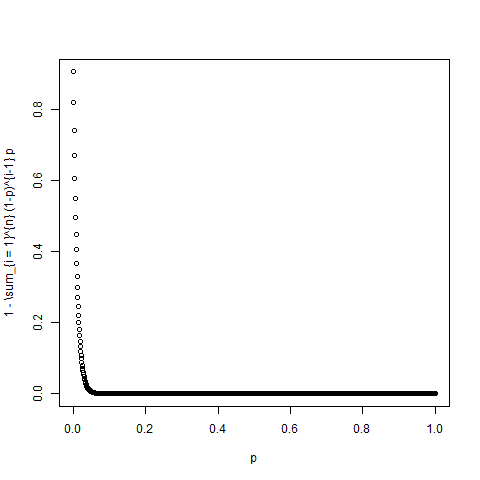
\includegraphics[width=6cm]{tarea2/problema2_1/graficas_inciso2_1_4/probabilidadDeQueC_pSupere100.png}
\end{center}\par\null

Con todo esto dicho, podemos garantizar que $C_p$ diverge a $\infty$ en distribución.\par\null

Entonces 
\begin{align}
    - \min_{n \leq C_p} \rightarrow - \min_{n \leq \infty} S_n = \min_{n \geq 0} S_n = M
\end{align}\par\null

Ahora recordemos que $g$ era una función continua y que $g>0$. Por lo tanto $1/g$ es una función continua,
con inverso derecho $f$ en $(0, 1)$. Es decir

Por lo tanto
\begin{align}
    \mw(M = n)  &=  \lim_{p \rightarrow 0} \mw(M_p = n)                         \\
                &=  \lim_{p \rightarrow 0} e^{-n f(1-p)}(1-e^{- f(1-p)})        \\
                &=   e^{-n f(1)}(1-e^{- f(1)}) \label{problema2_1:distribucion_de_M}
\end{align}

Lo cual corresponde a la distribución de una geométrica de parámetro $1-e^{- f(1)}$.\par\null

El caso donde $f(1^-) = 0$, implica que $\lim_{p\rightarrow0} (1-e^{- f(1-p)}) = 0$. El cual es complétamente
análogo al caso anterior donde considerábamos $p \rightarrow 0$ en geométricas de parámetro $p$.\par\null

Donde, habíamos dejado claro que conforme el parámetro disminuía hacia 0, las distribuciones de las geométricas divergía 
a la de $\infty$ y que por lo tanto la probabilidad de que nuestras geométricas tomaran cierto 
valor $n$ disminuía hacia $0$ conforme el parámetro tendía a $0$.\par\null

Incluso para este caso, la ecuación \eqref{problema2_1:distribucion_de_M} es válida según nuestro análisis, pues

\begin{align}
\mw(M = n)  &=  \lim_{p \rightarrow 0} \mw(M_p = n)                         \\
                &=  \lim_{p \rightarrow 0} e^{-n f(1-p)}(1-e^{- f(1-p)})    \\
                &=  e^{-n 0}(1-e^{- 0})                                     \\
                &=  1(1-1)                                                  \\
                &=  0.
\end{align}

Y esto, para toda $n \in \N$, justo como nuestro análisis de las distribuciones geométricas
nos dijo.
\end{proof}
\newpage

\section{Problema 2.2}  \label{problema2_2}
\begin{problema}
    \begin{enumerate}
        \item[(i)] 
            Instale \href{www.octave.org}{Octave} en su computadora
        \item[(ii)] 
            \'Echele un ojo a la documentaci\'on
        \item[(iii)] 
   
            Ejecute el siguiente c\'odigo linea por linea: 
            \textsl{
                    \lstinputlisting[caption=]{tarea2/problema2_2/polya1.R}
                    }
        \item[(iv)] 
            Lea las secciones sobre 
            \href{http://www.gnu.org/software/octave/doc/interpreter/Simple-Examples.html#Simple-Examples}{simple examples}, 
            \href{http://www.gnu.org/software/octave/doc/interpreter/Ranges.html#Ranges}{ranges}, 
            \href{http://www.gnu.org/software/octave/doc/interpreter/Random-Number-Generation.html#Random-Number-Generation}{random number generation} 
            y 
            \href{http://www.gnu.org/software/octave/doc/interpreter/Comparison-Ops.html#Comparison-Ops}{comparison operators} 
            y escriba su interpretaci\'on de lo que hace el c\'odigo anterior. Nota: est\'a relacionado con uno de los ejemplos del curso.
        \item[(v)] 
            Vuelva a correr el c\'odigo varias veces y escriba sus impresiones sobre lo que est\'a sucediendo.
    \end{enumerate}
\end{problema}

\afterstatement\par\null

En el código de arriba, se implementó una ejecución del proceso de las urnas de Poyla.\par\null

El vector \textsl{x} representa la proporción de las bolas ``verdes'' en la urna conforme el tiempo avanza. Que
al tiempo inicial se tenga \textsl{x=[1/2]} quiere decir que al inicio había tantas bolas ``verdes'' como ``rojas''.\par\null

Para octave los booleanos pueden operarse numéricamente. \textsl{true} es equivalente a \textsl{1} y
\textsl{false} es equivalente a \textsl{0}. Entonces, la parte que dice \\
\textsl{+(u(i)$<$x(i))} significa que se está sumando
uno o cero dependiendo de si la condición se satisface. 
Lo cual quiere decir que la constante de bolas que se agregan a la urna es $1$.\par\null

El vector \textsl{u} representa el resultado de sacar una bola. Si \textsl{u(i)$<$x(i)} significa que en el turno \textsl{i}, 
se obtuvo una bola ``verde''.\par\null

El \textsl{2} misterioso que se encuentra en varias partes significa que en el turno inicial existían \textsl{2} bolas en total.
Como al inicio la proporción era \textsl{1/2}, esto significa que al inicio existían una bola ``verde'' y una ``roja'' exactamente.\par\null

A continuación una gráfica obtenida de ejcutar el código.

\begin{center}
    \includegraphics[width=8cm]{tarea2/problema2_2/poyla.PNG}
\end{center}
\begin{center}
    Gráfica de una ejecución de urnas de Poyla \par\null
    1 bola verde inicial, 1 bola roja inicial y constante 1.
\end{center}\par\null

Se puede apreciar que conforme avanza el tiempo, la proporción de bolas ``verdes'' se estabiliza. Justo como se demostró en clase para
martingalas positivas (como la de este caso).
\newpage

\section{Problema 2.3}  \label{problema2_3}
\begin{problema}[Ejercicios sueltos sobre martingalas]
    \begin{enumerate}
        \item[(i)]        [\ref{problema2_3:inciso1}]
            Sea $\paren{X_n,n\geq 0}$ una sucesi\'on $\paren{\F_n}$-adaptada.\par
            Pruebe que        
            \begin{align}
                \sum_{k=1}^n X_k-\espc{X_k}{\F_{k-1}}, \quad n\geq 0
            \end{align}
            es una $\paren{\F_n}$-martingala.
        
        \item[(ii)]        [\ref{problema2_3:inciso2}]
            Descomposici\'on de Doob para submartingalas:\par
            Sea $X=\paren{X_n}_{n\in\na}$ una submartingala. 
            Pruebe que $X$ se puede descomponer de manera \'unica como $X=M+A$ donde $M$ es una martingala y $A$ 
            es un proceso previsible con $A_0=0$. Sugerencia: Asuma que ya tiene la descomposici\'on y calcule 
            esperanza condicional de $X_{n+1}$ dada $X_n$. 
        
        \item[(iii)]    [\ref{problema2_3:inciso3}]
            Sea $S_n=\xi_1+\cdots+\xi_n$ donde las variables $\xi$ son independientes y $\xi_i$ tiene 
            media cero y varianza finita $\sigma_i^2$. Pruebe que si $\sum_i \sigma_i^2<\infty$ entonces 
            $S_n$ converge casi seguramente y en $L_2$ conforme $n\to\infty$. Construya un ejemplo de 
            variables aleatorias $\xi_i$ tales que la serie $\sum_i \xi_i$ sea casi seguramente absolutamente 
            divergente y casi seguramente condicionalmente convergente (considere ejemplos simples!). 
            Explique heur\'isticamente por qu\'e cree que suceda esto.
            %Ser\'a que \sum_i\abs{x_i}=\infty casi seguramente si \sum_i\abs\esp{\xi_i}=\infty? 
        
        \item[(iv)]        [\ref{problema2_3:inciso4}]
            Sean $X$ y $Y$ dos martingalas (respecto de la misma filtraci\'on) y tales que $\esp{X_i},\esp{Y_i}<\infty$ 
            para toda $i$. Pruebe la siguiente f\'ormula de integraci\'on por partes: 
            \begin{align}
                \esp{X_nY_n}-\esp{X_0Y_0}=\sum_{i=1}^n \esp{\paren{X_i-X_{i-1}}\paren{Y_i-Y_{i-1}}}. 
            \end{align}
        
        \item[(v)]        [\ref{problema2_3:inciso4}]
            Desigualdad de Azema-Hoeffding, tomado de \cite[E14.2, p.237]{MR1155402}
            \begin{enumerate}
                \item[(v.i)] [\ref{problema2_3:subinciso5_1}]
                        Muestre que si $Y$ es una variable aleatoria con valores en $[-c,c]$ y 
                        media cero entonces, para $\theta\in\re$
                        \begin{align}
                            \esp{e^{\theta Y}}\leq\imf{\cosh}{\theta c}\leq \imf{\exp}{\frac{1}{2}\theta^2c^2}. 
                        \end{align}
                \item[(v.ii)] [\ref{problema2_3:subinciso5_2}]
                        Pruebe que si $M$ es una martingala nula en cero tal que para algunas 
                        constantes $\paren{c_n,n\in\na}$ se tiene que
                        \begin{align}
                            \abs{M_n-M_{n-1}}\leq c_n\quad\forall n
                        \end{align}
                        entonces, para $x>0$
                        \begin{align}
                            \proba{\max_{k\leq n} M_k\geq x}\leq \imf{\exp}{\frac{x^2}{2\sum_{k=1}^n c_k^2}}.
                        \end{align}
            \end{enumerate}
    \end{enumerate}
\end{problema}

\begin{proof}
    \subsection{Inciso (i)}        \label{problema2_3:inciso1}
    \emph{
    Sea $\paren{X_n,n\geq 0}$ una sucesi\'on $\paren{\F_n}$-adaptada. Pruebe que
    \begin{align}
        \sum_{k=1}^n X_k-\espc{X_k}{\F_{k-1}}, \quad n\geq 0
    \end{align}
    es una $\paren{\F_n}$-martingala.
}

\afterstatement\par\null

Nombremos $M_n = \sum_{k=1}^n X_k-\espc{X_k}{\F_{k-1}}, n \in \N$.\par\null

\begin{itemize}
	\item 
        Veamos que $(M_n)_{n \in \N}$ es $(\F_n)_{n \in \N}$-adaptada.\par\null
    
        $\sum_{k = 1}^n X_k$ es $\F_n$-medible por definición. $\E(X_k | \F_{k-1})$ es $\F_{k-1}$-medible por definición
        de esperanza condicional. \par\null
        
        Por lo tanto $\sum_{k = 1}^n \E(X_k | \F_{k-1})$ es $\F_{n-1}$-medible y por lo tanto
        $\F_n$-medible. Entonces
        
        \begin{align}
            \sum_{k = 1}^n X_k - \sum_{k = 1}^n \E(X_k | \F_{k-1}) &=  \sum_{k = 1}^n X_k - \E(X_k | \F_{k-1})    \\
                                                                    &=  M_n   
        \end{align}\par\null
    
        Es $\F_n$-medible. Como queríamos ver.\par\null
        
    \item
        Veamos que $M_n \in L_1$.\par\null
        
        Como no fue mencionado. Supondremos que $X_n \in L_1$. Si logramos demostrar que $\E(X_k | F_{k-1}) \in L_1$ habremos terminado.
        Puesto que $M_n$ sería suma finita de variables aleatorias en $L_1$ y por lo tanto pertenecería a $L_1$.\par\null
        
        \begin{align}
            \E(\abs{\E(X_k | F_{k-1})})     &\leq   \E(\E(\abs{X_k} | F_{k-1})) \\
                                            &=      \E(\abs{X_k}). 
        \end{align}
        
        Donde $\E(\abs{X_k})$ por supocisión es finita.\par\null
        
        Por lo tanto $\E(\abs{\E(X_k | F_{k-1})})$ también lo es, como queríamos demostrar.\par\null

\end{itemize}
    \newpage
    
    \subsection{Inciso (ii)}    \label{problema2_3:inciso2}
    \emph{
    Descomposici\'on de Doob para submartingalas: Sea $X=\paren{X_n}_{n\in\na}$ una submartingala. 
    Pruebe que $X$ se puede descomponer de manera \'unica como $X=M+A$ donde $M$ es una martingala y $A$ 
    es un proceso previsible con $A_0=0$. Sugerencia: Asuma que ya tiene la descomposici\'on y calcule 
    esperanza condicional de $X_{n+1}$ dada $X_n$. 
}

\afterstatement\par\null

$\paren{X_n}_{n\in\na}$ es $(\F_n)_{n \in \N}$-adaptada por definición de submartingala. Utilizando el inciso anterior tenemos
que $M_n = \sum_{k=1}^n X_k-\espc{X_k}{\F_{k-1}}, n \in \N$ es martingala.\par\null

%Ahora sea $M_n = N_n + X_0$. Veamos que $(M_n)_{n \in \N}$ sigue siendo martingala.
%
%\begin{itemize}
	%\item 
        %Veamos que $(M_n)_{n \in \N}$ es $(\F_n)_{n \in \N}$-adaptada.\par\null
        %
        %Por ser $(N_n)_{n \in \N}$ una martingala, $N_n$ es $\F_n$-medible y $X_0$ es 
        %$\F_0 \subset \F_n$-medible. Entonces $M_n$ es suma finita de variables $\F_n$-medibles y por lo tanto $\F_n$-medible.\par\null
    %
    %\item 
        %Veamos que $M_n \in L_1$ para toda $n \in \N$.\par\null
        %
        %Por ser $(N_n)_{n \in \N}$ una martingala, $N_n \in L_1$ para todo $n \in \N$. 
        %Por ser $(X_n)_{n \in \N}$ una subpartingala, $X_0 \in  L_1$.\par\null
        %
        %Por lo tanto $M_n$ es suma finita de variables en $L_1$ y por lo tanto pertenece a $L_1$.\par\null
    %
    %\item
        %Veamos que $\E(M_n | F_{n-1}) = M_{n-1}$.\par\null
        %
        %\begin{align}
            %\E(M_n | F_{n-1})   &=  \E(N_n + X_0 | F_{n-1})                     \\
                                %&=  \E(N_n | F_{n-1}) + \E( X_0 | F_{n-1})      \\
                                %&=  N_{n-1} + X_0                               \\
                                %&=  M_{n-1}.
        %\end{align}
        %
        %Y con esto terminamos de demostrar que $(M_n)_{n \in \N}$ es martingala.
%\end{itemize}

Si definimos a $A_n = X_n - M_n$ tendremos que $M_n + A_n = M_n + X_n - M_n = X_n$. Probemos ahora que
$(A_n)_{n \in \N}$ es previsible.\par\null

\begin{align}
    A_n     &=      X_n - M_n                                                                   \\
            &=      X_n - \sum_{k=1}^n X_k-\espc{X_k}{\F_{k-1}}                                 \\
            &=      X_n - X_n + \E(X_n | \F_{n-1}) + \sum_{k=1}^{n-1} X_k-\E(X_k|\F_{k-1})      \\     
            &=      \E(X_n | \F_{n-1}) + \sum_{k=1}^{n-1} X_k-\E(X_k|\F_{k-1}).     
\end{align}\par\null

Donde por ser $(X_n){n \in \N}$ submartingala tenemos que $\E(X_k|\F_{k-1})$ es $F_{n-1}$ siempre que $0 \leq k \leq n-1$.
Y por lo tanto $A_n$ es suma finita de variables $F_{n-1}$-medibles y por lo tanto $F_{n-1}$-medible.\par\null

Hemos demostrado hasta ahora que una submartingala se puede descomponer como la suma de una martingala y un proceso previsible.
Demostremos ahora la unicidad.\par\null

Sean entonces $M'_n$ y $A'_n$ una martingala y un proceso previsible respectivamente tal que $X_n = M'_n + A'_n$.\par\null

Entonces para toda $n \in \N$ tenemos que $M'_n + A'_n = M_n + A_n$. Por lo tanto 

\begin{align}
    (M'_n + A'_n) - (M'_{n+1} + A'_{n+1}) = (M_n + A_n) - (M_{n+1} + A_{n+1})
\end{align}\par\null

Tomemos esperanzas condicionales sobre el lado derecho.

\begin{align}
                                                    & \E((M_n + A_n) -( M_{n+1} + A_{n+1}) | \F_n)                                              \\ 
                                                    &=  \E((M_n + A_n) -( M_{n+1} + A_{n+1}) | \F_n)                                            \\
                                                    &=  \E(M_n - M_{n+1}| \F_n) + \E(A_n - A_{n+1} | \F_n)                                      \\
                                                    &=  M_n - M_{n} + \E(A_n - A_{n+1} | \F_n) \label{problema2_3:hipotesis_de_martingala}      \\
                                                    &=  \E(A_n - A_{n+1} | \F_n)                                                                \\
                                                    &=  \E(A_n| \F_n) - \E(A_{n+1} | \F_n)                                                      \\
                                                    &=  A_n - A_{n+1} \label{problema2_3:hipotesis_de_proceso_previsible}                                                                               
\end{align}\par\null

Donde \eqref{problema2_3:hipotesis_de_martingala} es gracias a que $(M_n)_{n\in\N}$ es martingala y \eqref{problema2_3:hipotesis_de_proceso_previsible}
es gracias a que $(A_n)_{n\in\N}$ es un proceso previsible.\par\null

De manera análoga obtenemos que $\E((M'_n + A'_n) - (M'_{n+1} + A'_{n+1}) | \F_n) = A'_n - A'_{n+1}$ y por lo tanto $A_n - A_{n+1} = A'_n - A'_{n+1}$.\par\null

Lo que esto último dice, es que $(A_n)_{n\in\N}$ y $(A'_n)_{n\in\N}$ crecen igual. Recordemos que por hipótesis $A'_0, A_0 = 0$.\par\null

Entonces
\begin{align}
    A_0 - A_1 &= A'_0 - A'_1 &\Rightarrow A_1 &= A'_1
\end{align}\par\null

Inductivamente, si $A_n = A'_n$, entonces
           
\begin{align}
    A_n - A_{n+1} &= A'_n - A'_{n+1} &\Rightarrow A_{n+1} &= A'_{n+1}
\end{align}                                                                                                         

Y con esto queda demostrada la unicidad de $(A_n)_{n\in\N}$. Para la demostración de la unicidad de $M_n$, sólo recordemos que 
$M_n = X_n - A_n$ y que $M'_n = X_n - A'_n$, por ser $A_n$ y $A'_n$ iguales, entonces $M_n$ y $M'_n$ también lo son.
    \newpage
        
    \subsection{Inciso (iii)}    \label{problema2_3:inciso3}
    \emph{
    Sea $S_n=\xi_1+\cdots+\xi_n$ donde las variables $\xi$ son independientes y $\xi_i$ tiene 
    media cero y varianza finita $\sigma_i^2$. Pruebe que si $\sum_i \sigma_i^2<\infty$ entonces 
    $S_n$ converge casi seguramente y en $L_2$ conforme $n\to\infty$. Construya un ejemplo de 
    variables aleatorias $\xi_i$ tales que la serie $\sum_i \xi_i$ sea casi seguramente absolutamente 
    divergente y casi seguramente condicionalmente convergente (considere ejemplos simples!). 
    Explique heur\'isticamente por qu\'e cree que suceda esto.
    %Ser\'a que \sum_i\abs{x_i}=\infty casi seguramente si \sum_i\abs\esp{\xi_i}=\infty? 
}

\afterstatement\pn

Sea $\F_n = \sigma( \xi_0, \xi_1, \dots, \xi_n)$.\pn


Probemos ahora que $(S_n)_{n \in \N}$ es martingala con respecto de la \newline 
filtración $(\F_n)_{n \in \N}$.\pn

Por como se definió $\F_n$, $S_n$ es $\F_n$-medible. Por otra parte, $S_n$ es suma finita de variables en $L_1$ 
(pues las $\xi_i$'s tienen esperanza finita).\pn

Ahora
\begin{align}
    \E(S_{n+1} | \F_n)  &=  \E(\xi_{n+1} | \F_n) + \E(S_n | \F_n)                       \\
                        &=  \E(\xi_{n+1} | \F_n) + S_n                                  \\
                        &\;\;\;\;\mbox{Porque $S_n$ es $F_n$-medible}                   \\
                        &=  \E(\xi_{n+1}) + S_n                                         \\
                        &\comment{Porque $\xi_{n+1}$ es independiente de$F_n$}        	\\
                        &=  0 + S_n.                                                    \\
\end{align}\pn

Y con esto hemos demostrado que $S_n$ es martingala.\pn

Ahora, como $\E(\xi_n) = 0$ para todo $n \in \N$, $\E(S_n) = 0$ para todo $n \in \N$.

\begin{align}
        \var{S_n}       &=  \E(S_n^2) - \E(S_n)^2                                               \\
                        &=  \E(S_n^2) - 0                                                       \\
                        &=  \sum_{i \leq n} \sigma_i^2                                          \\
                        &\comment{Esto último gracias a que los $\xi_i$'s son independientes}.
\end{align}

Ahora $\| S_n \|_2 = \sqrt{\var{S_n}} = \sqrt{\sum_{i \leq n} \sigma_i^2}$. Recordemos que por ser  $\sqrt{\cdot}$
función continua, manda sucesiones convergentes en sucesiones convergentes. Como 
$\lim\limits_{n \rightarrow \infty} \sum\limits_{i < n} \sigma_i^2 < \infty$, 
entonces $\lim\limits_{n \rightarrow \infty}\| S_n \|_2 < \infty$.\pn

En particular, $\sup\limits_n \| S_n \|_2 < \infty$.\pn

El teorema de convergencia en $L_p$ de Doob nos garantiza que $S_n$ converge casi seguramente y en $L_2$. Como queríamos
hacer ver.\pn

Definamos ahora $\xi_i$ con $\mw(\xi_i = \pm \frac{1}{i+1}) = \frac{1}{2}$.

Dado que la serie $\sum_{n \geq 1} \frac{1}{n}$ es divergente. $S_n$ es absolutamente divergente casi seguramente.\pn

Ahora, $\E(\xi_i) = \frac{1}{2(i+1)}-\frac{1}{2(i+1)} = 0$ y $\var{\xi_i} = \frac{1}{(i+1)^2}$. Entonces, por lo dicho en la primera
parte de este ejercicio, $S_n$ converge casi seguramente y en $L_2$. Es decir que la serie $S_n$ converge condicinalmente casi seguramente.\pn

Heurísticamente, para que la serie diverja es necesario mantener el mismo signo por periodos ``muy largos''. La probabilidad de mantener el 
mismo signo por mucho tiemp decrece exponencialmente. Por eso es razonable que si elegimos en base a volados los signos de los términos,
la serie terminará convergiendo.
    \newpage
    
    \subsection{Inciso (iv)}    \label{problema2_3:inciso4}
    \emph{
    Sean $X$ y $Y$ dos martingalas (respecto de la misma filtraci\'on) y tales que $\esp{X_i},\esp{Y_i}<\infty$ 
    para toda $i$. Pruebe la siguiente f\'ormula de integraci\'on por partes: 
    \begin{align}
        \E{X_nY_n}-\E{X_0 Y_0}=\sum_{i=1}^n \E{\paren{X_i-X_{i-1}}\paren{Y_i-Y_{i-1}}}. 
    \end{align}
}

\afterstatement\pn

Descompongamos $\sum_{i \leq n} \E((X_i - X_{i-1}) (Y_i - Y_{i-1}))$

\begin{align}
    &\sum_{1 \leq i \leq n} \E((X_i - X_{i-1}) (Y_i - Y_{i-1}))                                                                         \\
    &=  \sum_{1 \leq i \leq n} \E(X_i Y_i - X_i Y_{i-1} - X_{i-1} Y_i + X_{i-1} Y_{i-1})                                                \\
    &=  \sum_{1 \leq i \leq n} \E(X_i Y_i) - \E(X_i Y_{i-1}) - \E(X_{i-1} Y_i) + \E(X_{i-1} Y_{i-1})                                    \\
    &=  \sum_{1 \leq i \leq n} \E(X_i Y_i) - \E(\E(X_i Y_{i-1}) | \F_{i-1}) - \E(\E(X_{i-1} Y_i) | \F_{i-1}) + \E(X_{i-1} Y_{i-1})      \\
    &=  \sum_{1 \leq i \leq n} \E(X_i Y_i) - \E(Y_{i-1} \E(X_i | \F_{i-1})) - \E(X_{i-1}\E(Y_i | \F_{i-1})) + \E(X_{i-1} Y_{i-1})       \\
    &\comment{Esto último gracias a que $X_{i-1}, Y_{i-1}$ son $F_{i-1}$ medibles}                                                      \\
    &=  \sum_{1 \leq i \leq n} \E(X_i Y_i) - \E(Y_{i-1} X_{i-1}) - \E(X_{i-1} Y_{i-1}) + \E(X_{i-1} Y_{i-1})                            \\
    &\comment{Esto último gracias a que $X,Y$ son martingalas}                                                                          \\
    &=  \sum_{1 \leq i \leq n} \E(X_i Y_i) - \E(Y_{i-1} X_{i-1})                                                                        
\end{align}\pn

En esta última suma podemos notar que se trata de una telescópica, y por lo tanto

\begin{align}
    \sum_{1 \leq i \leq n} \E((X_i - X_{i-1}) (Y_i - Y_{i-1})) &=  \E(X_n Y_n) - \E(Y_{0} X_{0}).
\end{align}\pn

Que es precisamente lo que buscábamos demostrar.
    \newpage
    
    \subsection{Inciso (v)}        \label{problema2_3:inciso5}
    Desigualdad de Azema-Hoeffding, tomado de \par
\cite[E14.2, p.237]{MR1155402}\par\null

\begin{enumerate}
    \item[(v.i)]    [\ref{problema2_3:subinciso5_1}]
         Muestre que si $Y$ es una variable aleatoria con valores en $[-c,c]$ y media cero entonces, para $\theta\in\re$
        
        \begin{align}
            \esp{e^{\theta Y}}\leq\imf{\cosh}{\theta c}\leq \imf{\exp}{\frac{1}{2}\theta^2c^2}. 
        \end{align}\par\null

    \item[(v.ii)]    [\ref{problema2_3:subinciso5_2}]
        Pruebe que si $M$ es una martingala nula en cero tal que para algunas constantes $\paren{c_n,n\in\na}$ se tiene que
        
        \begin{align}
            \abs{M_n-M_{n-1}}\leq c_n\quad\forall n
        \end{align}
        
        entonces, para $x>0$
        
        \begin{align}
            \proba{\max_{k\leq n} M_k\geq x}\leq \imf{\exp}{\frac{x^2}{2\sum_{k=1}^n c_k^2}}.
        \end{align}
\end{enumerate}
    
\subsubsection{Subinciso (v.1)}     \label{problema2_3:subinciso5_1}
    \input{tarea2/problema2_3/subinciso2_3_5_1.tex}
    \newpage
    
\subsubsection{Subinciso (v.ii)}    \label{problema2_3:subinciso5_2} 
    \input{tarea2/problema2_3/subinciso2_3_5_2.tex}


\end{proof}
\newpage

\section{Problema 2.4}  \label{problema2_4}
\begin{problema}
    Sea $S_n=\sum_{i=1}^n X_i$ donde $X_1,X_2,\ldots$ son iid. Sea
    
    \begin{align}
        \imf{\phi}{\lambda}=\esp{e^{\lambda S_n}}\in (0,\infty].
    \end{align}

    \begin{enumerate}
        \item[(i)]		[\ref{problema2_4:inciso1}]
            Pruebe que si existen $\lambda_1<0<\lambda_2$ tales que $\imf{\phi}{\lambda_i}<\infty$ entonces $\imf{\phi}{\lambda}<\infty$ 
			para toda $\lambda\in [\lambda_1,\lambda_2]$. Sugerencia: escriba $\lambda=a\lambda_1+(1-a)\lambda_2$ para alg\'un $a\in [0,1]$ 
			y aplique la desigualdad de H\"older. A partir de ahora se asume la premisa de este inciso.\pn
			
        \item[(ii)] 	[\ref{problema2_4:inciso2}]
            Pruebe que $\esp{\abs{S_n}^k}<\infty$ para toda $k\geq 0$.\pn
			
        \item[(iii)] 	[\ref{problema2_4:inciso3}]
            Sea $M^\lambda_t=e^{\lambda S_t}/\imf{\phi}{\lambda}$. Argumente que si $M^n$ es el proceso dado por
            
            \begin{align}
                M^n_t=\left.\frac{\partial^n}{\partial \lambda^n}\right|_{\lambda=0}M^\lambda_t,
            \end{align}
            
            entonces $M^n$ es una martingala para toda $n$. \pn
        %\item[(iv)] 	[\ref{problema2_4:inciso4}]
            %Calcule las primeras $4$ martingalas resultantes si $\proba{X_i=\pm 1}=1/2$. Util\'icelas para calcular el valor de $\esp{T^2}$ donde
%
            %\begin{align}
                %T=\min\set{n\geq 0: S_n\in\set{-a,b}}
            %\end{align}y $a,b>0$.\pn 
    \end{enumerate}

    \defin{Categor\'ias:} Caminatas aleatorias, muestreo opcional, ejemplos de martingalas. 
\end{problema}

\begin{proof}
    \subsection{Inciso (i)}     \label{problema2_4:inciso1}
    \emph{
	Pruebe que si existen $\lambda_1<0<\lambda_2$ tales que $\imf{\phi}{\lambda_i}<\infty$ entonces $\imf{\phi}{\lambda}<\infty$ 
	para toda $\lambda\in [\lambda_1,\lambda_2]$. Sugerencia: escriba $\lambda=a\lambda_1+(1-a)\lambda_2$ para alg\'un $a\in [0,1]$ 
	y aplique la desigualdad de H\"older. A partir de ahora se asume la premisa de este inciso.
}

\afterstatement\pn

Sea $\lambda = \lambda_1 (1-t) + \lambda_2 t$ con $t \in [0, 1]$. Por lo tanto 

\begin{align}
    \phi(\lambda)   &= \E(e^{\lambda S_n})                                              \\
                    &= \E\paren{e^{(\lambda_1 (1-t) + \lambda_2 t) S_n}}                \\
                    &= \E\paren{e^{(\lambda_1 (1-t) S_n + \lambda_2 tS_n) }}            \\  
                    &= \E\paren{e^{\lambda_1 (1-t) S_n} e^{\lambda_2 tS_n) }}           \\  
                    &= \E\paren{{e^{(\lambda_1 S_n)}}^{1-t} {e^{(\lambda_2 S_n)}}^t}      
\end{align}

Si definimos $p = 1/(1-t)$ y $q = 1/t$, tenemos que
${e^{(\lambda_1 S_n)}}^{1-t} \in L_p$ pues $\paren{{e^{(\lambda_1 S_n)}}^{1-t}}^p = e^{(\lambda_1 S_n)}$ quien 
pertenece a $L_1$ por hipótesis. Análgomanente tenemos que  ${e^{(\lambda_2 S_n)}}^t \in L_q$.\pn

Ahora, recordando que $|e^x| = e^x$ y utilizando la desigualdad de Hölder \eqref{Desigualdad_de_Holder}

\begin{align}
    \phi(\lambda)   &=      \E\paren{{e^{(\lambda_1 S_n)}}^{1-t} {e^{(\lambda_2 S_n)}}^t}           \\      
                    &\leq   \E\paren{e^{(\lambda_1 S_n)}}^{1-t} \E\paren{e^{(\lambda_2 S_n)}}^t     
\end{align}\pn

Donde cada uno de los factores es finito por hipótesis y por lo tanto $\phi(\lambda) < \infty$. Como queríamos demostrar.
    \newpage
    
    \subsection{Inciso (ii)}    \label{problema2_4:inciso2}
    \emph{
	Pruebe que $\esp{\abs{S_n}^k}<\infty$ para toda $k\geq 0$.
}

\afterstatement\par\null

Ahora que sabemos que si $\lambda \in [\lambda_1, \lambda_2]$ entonces $\phi(\lambda) < \infty$. Elijamos 
$\lambda = \min(-\lambda_1, \lambda_2)$ y de esta manera, tenemos que $\phi(-\lambda), \phi(\lambda) < \infty$.\par\null

Entonces

\begin{align}
    \E(e^{|\lambda S_n|})   &=      \E(e^{\lambda S_n} \indic_{\lambda S_n \geq 0} + e^{-\lambda S_n} \indic_{\lambda S_n < 0} )        \\ 
                            &=      \E(e^{\lambda S_n} \indic_{\lambda S_n \geq 0}) + \E(e^{-\lambda S_n} \indic_{\lambda S_n < 0})     \\
                            &\leq   \E(e^{\lambda S_n} ) + \E(e^{-\lambda S_n})                                                         \\
                            &=      \phi(\lambda) + \phi(-\lambda)                                                                      \\
                            &<      \infty.                                                  
\end{align}\par\null

Este hecho lo necesitaremos más adelante.\par\null
    \newpage
        
    \subsection{Inciso (iii)}    \label{problema2_4:inciso3}
    \emph{
	Sea $M^\lambda_t=e^{\lambda S_t}/\imf{\phi}{\lambda}$. Argumente que si $M^n$ es el proceso dado por
	\null
	\begin{align}
		M^n_t=\left.\frac{\partial^n}{\partial \lambda^n}\right|_{\lambda=0}M^\lambda_t,
	\end{align}
	\null
	entonces $M^n$ es una martingala para toda $n$.
}

\afterstatement\pn
    \newpage
    
    %\subsection{Inciso (iv)}    \label{problema2_4:inciso4}
    %\emph{
	Si $\proba{X_i=\pm 1}=1/2$, calcule las primeras $4$ martingalas resultantes.
    Util\'icelas para calcular el valor de $\esp{T^2}$ donde
    \null
	\begin{align}
		T=\min\set{n\geq 0: S_n\in\set{-a,b}}
	\end{align}
    \null
    y $a,b>0$.
}

\afterstatement\par\null
\end{proof}        
        \nqed
        
    \part{Tarea 3}
        \section{Problema 3.1}  \label{problema3_1}
\begin{problema}
Sea $M$ una $\paren{\F_n}$-martingala. Pruebe que si $T$ es un tiempo de paro finito entonces $\esp{M_T}=\esp{M_0}$ bajo cada una de las siguientes condiciones:
\begin{enumerate}
    \item[(i)] \ref{problema3_1:inciso1}
        $M$ es acotada.
    \item[(ii)] \ref{problema3_1:inciso2}
        $T$ es integrable y la sucesi\'on $\paren{M_n-M_{n-1}}$ es acotada.
    \item[(iii)] \ref{problema3_1:inciso3}
        $\paren{M_{n\wedge T}}$ es uniformemente integrable. 
\end{enumerate}

\defin{Categor\'ias: } Muestreo opcional.
\end{problema}

\begin{proof}
    \subsection{Inciso (i)}     \label{problema3_1:inciso1}
    \emph{
    $M$ es acotada.
}

\afterstatement\pn

Que $M$ sea acotada significa que existen $a \in  \R$ tal que $\abs{M_n} < r$ para todo $n \in \N$. En particular 
tenemos que $\abs{M_{T \wedge n}} < r$.\pn

Por otro lado, que $T$ sea finito implica que $T \wedge n  \underset{c.s.}\longrightarrow T$ conforme $n \rightarrow \infty$.
(Para todo $\omega \in \Omega$, $T(\omega) = n_0 < \infty$ y por lo tanto $T \wedge n (\omega) = T(\omega) = n_0$ para todo
$n \geq n_0$). De donde afirmamos que $M_{T \wedge n} \underset{c.s.}\longrightarrow M_T$. \pn

Ahora, $T \wedge n$ es tiepo de paro acotado, y por Teorema del Muestreo Opcional de Doob tenemos que 
$\E(M_{T \wedge n}) = \E(M_0)$.\pn

Tenemos todas las hipótesis para aplicar el Teorema de Convergencia Acotada y por lo tanto:

\begin{align}
    \E(M_T)     &=  \E\left(\lim_{n \rightarrow \infty} M_{T \wedge n}\right)       \\
                &=  \lim_{n \rightarrow \infty} \E(M_{T \wedge n})                  \\
                &=  \E(M_0).
\end{align}\pn

Con lo que termina la demostración.
 
    \newpage
    
    \subsection{Inciso (ii)}    \label{problema3_1:inciso2}
    \emph{
    $T$ es integrable y la sucesi\'on $\paren{M_n-M_{n-1}}$ es acotada.
}

\afterstatement\pn

Que la sucesión $\paren{M_n-M_{n-1}}$ sea acotada, significa que existe $r \in R$ tal que
$\abs{M_n - M_{n-1}} < r$ para todo $n \geq 1$.\pn

Que $T$ sea integrable significa que $\E(T) < \infty$. Recordemos que el que $T$ sea finito implica que 
$T \wedge n \underset{c.s.}\longrightarrow T$ (la justificación está en \ref{problema3_1:inciso1}). \pn

Otra vez, $T \wedge n$ es tiepo de paro acotado, y por Teorema del Muestreo Opcional de Doob tenemos que 
$\E(M_{T \wedge n}) = \E(M_0)$. En este caso nos conviene escribirlo de la siguiente manera, 
$\E(M_{T \wedge n} - M_0) = 0$.\pn

Ahora, 
\begin{align}
    \abs{M_{T \wedge n} - M_0}  &=      \abs{\sum_{1 \leq i \leq (T \wedge n)} (M_i - M_{i-1})}     \\
                                &\leq   \sum_{1 \leq i \leq (T \wedge n)} \abs{(M_i - M_{i-1})}     \\
                                &\leq   (T \wedge n) r                                              \\      
                                &\leq   T r                                                    
\end{align}

De donde 

\begin{align}
        \E(\abs{M_{T \wedge n} - M_0})  &\leq   \E(T r) \\
                                        &= r \E(T)      \\
                                        &< \infty.
\end{align} \pn

Con esto tenemos que la sucesión $(M_{T \wedge n} - M_0)_{n \in \N}$ es dominada por $Tr$ y que cada 
elemento de la sucesión es integrable. Entonces tenemos todas las hipótesis del Teorema de convergencia dominada.
Y por lo tanto

\begin{align}
        \E(M_T - M_0)   &=  \E(\lim_{n \rightarrow \infty} M_{T \wedge n} - M_0)        \\
                        &=  \lim_{n \rightarrow \infty} \E(M_{T \wedge n} - M_0)        \\
                        &=  \lim_{n \rightarrow \infty} 0                               \\
                        &=  0.                        
\end{align}\pn

Lo cual implica $\E(M_T) = \E(M_0)$, como queríamos demostrar.
    \newpage
        
    \subsection{Inciso (iii)}    \label{problema3_1:inciso3}
    \emph{
    $\paren{M_{n\wedge T}}$ es uniformemente integrable. 
}

Sabemos que $M_{T \wedge n} \underset{c.s.}\longrightarrow M_T$ gracias a que $T$ es finito 
(la justificación está en \ref{problema3_1:inciso1}).\pn

Existe un teorema que garantiza que si $M_{T \wedge n} \underset{c.s.}\longrightarrow M_T$ y 
$\paren{M_{n\wedge T}}$ es uniformemente integrable, entonces 
$M_T \in L_1$ y $M_{T \wedge n} \underset{L_1}\longrightarrow M_T$.\pn

Es decir que $\E(M_{T \wedge n}) \longrightarrow \E(M_T)$, y de nueva cuenta, por Teorema del Muestreo Opcional de Doob, 
en vista que $T \wedge n$ es tiempo de paro acotado, tenemos que $\E(M_{T \wedge n}) = \E(M_0)$ y por lo tanto

\begin{align}
    \E(M_T)     &=  \lim_{n \rightarrow \infty} \E(M_{T \wedge n})      \\
                &=  \lim_{n \rightarrow \infty} \E(M_0)                 \\
                &=  \E(N_0).
\end{align}\pn

Que es lo que buscábamos demostrar.

    \newpage
\end{proof}
\newpage

\section{Problema 3.2}  \label{problema3_2}
\begin{problema}
    Sea $M$ una $\paren{\F_n}$-martingala con saltos acotados. Sean

    \begin{align}
    C   &=  \set{\limsup M_n=\liminf M_n\in\re}                 \\
        &y                                                      \\
    D   &=  \set{\limsup M_n=-\infty\text{ y }\limsup M_n=\infty}.
    \end{align}\par\null

    Pruebe que $\proba{C\cup D}=1$. Deduzca que las caminatas aleatorias centradas 
    con saltos acotados oscilan. Sugerencia: Para cada $K>0$ defina

    \begin{align}
    T=\min\set{n\geq 0: \abs{M_n}\geq K}
    \end{align}

    y aplique el teorema de convergencia de martingalas a $M^T$.\par\null

    Sea $M$ una caminata aleatoria no trivial con saltos integrables en 
    $-1,0,1,\ldots$ y  media cero.\par\null 

    Pruebe que $\proba{M\text{ converge en }\na}=0$ y  concluya que $\liminf M_n=-\infty$ 
    casi seguramente. (Este resultado permitir\'a dar una prueba adicional de que un Galton-Watson cr\'itico se extingue).  
    Sugerencia: proceda como en el párrafo anterior y pruebe la integrabilidad uniforme de $(M_{T\wedge n})_{n \in \N}$.

    \defin{Categor\'ias: } Teoremas de convergencia de martingalas
\end{problema}

\afterstatement\par\null

Definamos 

\begin{align}
    T_k = \min\{ n \geq 0 : \abs{M_n} \geq k \}.
\end{align}

Que significa ``la primera vez que la martingala se aleja de cero al menos $k$ unidades''. 
Veamos que se trata de un tiempo de paro.


\begin{align}
    \{ T_k = n \}   &=  \paren{\bigcup_{i \leq n-1} \{ \abs{M_i} < k \}} \cap \paren{\{ \abs{M_n} \geq k \}}                                 \\
                    &=  \paren{\bigcap_{i \leq n-1} \{ M_i < k \} \cap \{ M_i > -k \}} \cap \paren{\{ M_n \geq k \} \cup \{ M_n \leq -k \}}.
\end{align}\par\null

Donde, $\{ M_i < k \}, \{ M_i > -k \} \in \F_i \subset \F_n$ y $\{ M_n \geq k \}, \{ M_n \leq -k \} \in \F_n$. 
Y por lo tanto $\{ T_k = n\} \in \F_n$, de donde concluimos que $T_K$ es efectivamente tiempo de paro.\par\null


Sea $C$ una cota para los saltos de $M$. Por definición de $T_k$, es claro que para el tiempo $T_k$ (cuando $T_k$ es finito), 
la martingala se aleja en al menos $k$ unidades de 0, pero forzosamente menos que $k + C$, pues su último salto no 
puede superar $C$. Es decir $\abs{M_{T_k}} < k + C$. Pero esto únicamente será cierto en los casos en que $T_k$ resulte 
ser finito. Tomemos en cuenta entonces al tiempo $T_k \wedge n$, qué satisface ser finito y que $T_k \wedge n \leq T_k$. 
Para este tiempo, nuestro razonamiento anterior es válido y entonces tenemos $\abs{M_{T_k \wedge n}} < k + C$.\par\null

Entonces $\E(\abs{M_{T_k \wedge n}}) < \E(k + C) = k + C$ para toda $n \in N$. Sabemos de [\ref{problema1_4}] que 
$(M_{T_k \wedge n})_{n \in \N}$ es martingala. Por el Teorema de Convergencia de Martingalas, tenemos que 
$M_{T_k \wedge n} \longrightarrow M_{T_k}$ y es finita c.s.\par\null

Estudiemos ahora los casos de convergencia de la martingala. Definimos

\begin{align}
        A_1     &=  \{ \limsup M_n < \infty     \}    \\
        A_2     &=  \{ \liminf M_n > -\infty    \}
\end{align}

Estos son los casos donde la martingala no se dispara hacia arriba indefinidamente o hacia abajo indefinidamente
(respectivamente).\par\null

Los casos que queremos estudiar son $B_1 = A_1 \cap A_2$, $B_2 = A_1^c \cap A_2$, $B_3 = A_1 \cap A_2^c$ y 
$B_4 = A_1^c \cap A_2^c$. Es decir que $B_1$ es el caso donde la caminata se queda acotada. $B_2$ Es el caso 
donde la caminata alcanza todos los niveles arriba de cero. $B_3$ el caso donde la caminata alcanza todos 
los niveles abajo de cero. Y $B_4$ es el caso en el que la caminata oscila (alcanza todos los niveles).\par\null

Del análisis anterior, podemos ver que $B_2$ y $B_3$ tienen probabilidad 0, pues en estos casos, el límite de
$M_n$ es infinito y nuesto análisis mostró que la variable aleatoria a la que se converge es finita casi seguramente.\par\null

De esto tenemos que $\mw(D \cup C) = 1$, pues $C \subset B_1$ y $D = B_4$ en la manera que definimos a $B_1$ y $B_4$.\par\null

Ahora, notemos que $A_1, A_2 \subset \bigcup_{k \in \N} \{ T_k = \infty \}$. Del análisis anterior tenemos que 
en $\{ T_k = \infty \}$, nuestra caminata converge casi seguramente, y por lo tanto también converge casi seguramente
en $A_1$ y en $A_2$ (es decir, en $B_1$).\par\null




\newpage

\section{Problema 3.3}  \label{problema3_3}
\begin{problema}
Sean $X_1,X_2,\ldots$ variables aleatorias intercambiables:\begin{esn}
\paren{X_1,\ldots, X_n}\stackrel{d}{=}\paren{X_{\pi_1},\ldots, X_{\pi_n}}
\end{esn}para cada permutaci\'on $\sigma$ de $\set{1,\ldots,n}$. 
\begin{enumerate}
\item Para $\G,\h$ sub$\sigma$-\'algebras de $\F$ definimos a $\G\vee\h=\sag{\G\cup\h}$. Sea \begin{esn}
\G^n=\sag{\imf{f}{X_1,\ldots, X_n}: \fun{f}{\re^n}{\re}\text{ es sim\'etrica}}\vee\sag{X_{n+1},X_{n+2},\ldots}. 
\end{esn}Pruebe que $\G^n,n\geq 1$ es una filtraci\'on al rev\'es. Sea $\G$ su intersecci\'on.
\item Para cada $A\in\mc{B}_{\re}$, defina a\begin{esn}
\imf{\Xi_n}{A}=\frac{1}{n}\sum_{i=1}^n \indi{X_i\in A}.
\end{esn}Pruebe que\begin{esn}
\probac{X_1\in A}{\G^n}=\imf{\Xi_n}{A}. 
\end{esn}?`Por qu\'e puede definir a  $\imf{\Xi}{A}=\lim_{n\to\infty}\imf{\Xi_n}{A}$?
\item Al considerar a la martingala\begin{esn}
\frac{1}{n\paren{n-1}}\sum_{1\leq i<j\leq n}\indi{X_i\in A}\indi{X_j\in A},
\end{esn}pruebe que $\probac{X_1\in A,X_2\in A}{\G}=\probac{X_1\in A}{\G}\probac{X_2\in A}{\G}$. Extienda la afirmaci\'on de independencia condicional anterior a $X_1,\ldots, X_n$. 
\end{enumerate}

\defin{Cagegor\'ias: }Teorema de convergencia de martingalas, variables intercambiables, teorema de de Finetti.
\end{problema}
\newpage

\section{Problema 3.4}  \label{problema3_4}
\begin{problema}
\mbox{}
    \begin{enumerate}
        \item[(i)]	[\ref{problema3_4:inciso1}]
            Ejecute y explique la funci\'on del siguiente c\'odigo en Octave. Comente qu\'e 
            teoremas del curso (y del curso de probabilidad) son importantes para interpretar 
            la figura.
            \tiny
            \texttt
            {
                \lstinputlisting[caption=]{tarea3/problema3_4/polya2.R}
            }
            \normalsize
            (Conmigo se negó a brincar de linea. Tuve que hacerlo diminuto para que apareciera el código completo.)\pn
        
        \item[(ii)]	[\ref{problema3_4:inciso2}]
            Ejecute y explique la funci\'on del siguiente c\'odigo en Octave. 
            Incluya una gr\'afica en la que la longitud de la variable k sea mayor a 1000. 
            (Puede modificar el programa...) En la gr\'afica observara un esbozo de la 
            trayectoria de un proceso de ramificaci\'on continuo (en una escala distinta...).
            \texttt{
                \lstinputlisting[caption=]{tarea3/problema3_4/binaryGW.R}
            }
    \end{enumerate}
\end{problema}

\begin{proof}
    \subsection{Inciso (i)} \label{problema3_4:inciso1}
    \emph
{
            Ejecute y explique la funci\'on del siguiente c\'odigo en Octave. Comente qu\'e 
            teoremas del curso (y del curso de probabilidad) son importantes para interpretar 
            la figura.
            \tiny
            \texttt
            {
                \lstinputlisting[caption=]{tarea3/problema3_4/polya2.R}
            }
            \normalsize
}

\afterstatement\pn

En el código se simulan \texttt{10000} procesos de urnas de Póyla con \texttt{1000} iteraciones cada uno.\pn

\texttt{n} es el número de juegos por proceso.\pn

\texttt{m} es el número de simulaciones.\pn

\texttt{u} es una matriz de probabilidades. En este caso, la 
entrada \texttt{(i,j)}, es el ``resultado'' del turno
\texttt{j} en el proceso \texttt{i}.\pn

\texttt{r} y \texttt{v} son el número de pelotas rojas y verdes 
(respectivamente) con las que comienza cada proceso. Esto se deduce 
de la manera en que se obtienen las proporciones iniciales \texttt{r/(r+v)}.\pn

\texttt{c} es la constante de bolas que se agregan en cada paso del proceso. Esto se deduce en la manera que se obtiene la
\texttt{i}-ésima proporción (se divide entre \texttt{r+v+i*c} es decir, el número de pelotas en el \texttt{i}-ésimo paso es
el número de bolas iniciales más \texttt{i} veces \texttt{c}).\pn

\texttt{x} es una matriz en cuyas columnas se representan la sucesión de proporciones de 
bolas rojas en cada proceso. La instrucción \texttt{ones(1,m)} genera una matriz de 
\texttt{1$\times$m} con unos en todas las entradas. Al multiplicar por \texttt{r/(r+v)} 
se obtiene una matriz con el valor \texttt{r/(r+v)} en todas sus entradas. En otras palabras, 
\texttt{x} es el vector de proporciones de bolas rojas iniciales para cada proceso.\pn

El ciclo \texttt{for} es para calcular las sucesiones de proporciones. Se puede comparar 
con el del problema [\ref{problema2_2}] o
su versión corregida que se encuentra en la solución de dicho problema.\pn

\texttt{y} es la colección de proporciones de bolas rojas finales de cada proceso. Para 
fines de graficación, se ordenan con el
comando \texttt{sort}.\pn

En la penúltima linea se ve el comando \texttt{plot} a quien se le pasan la colección 
de proporciones finales y una representación de una función beta con parámetros de forma 
(shape parameters) \texttt{r/c} y \texttt{v/c}.\pn

La siguiente gráfica es el resultado de una ejecución del algoritmo anterior. En azul, se 
muestra el resultado experimental de las \texttt{10000} iteraciones del proceso. En verde 
la gráfica de una distribución Beta con parámetros de forma \texttt{r/c} y \texttt{v/c}.\pn

\begin{center}
    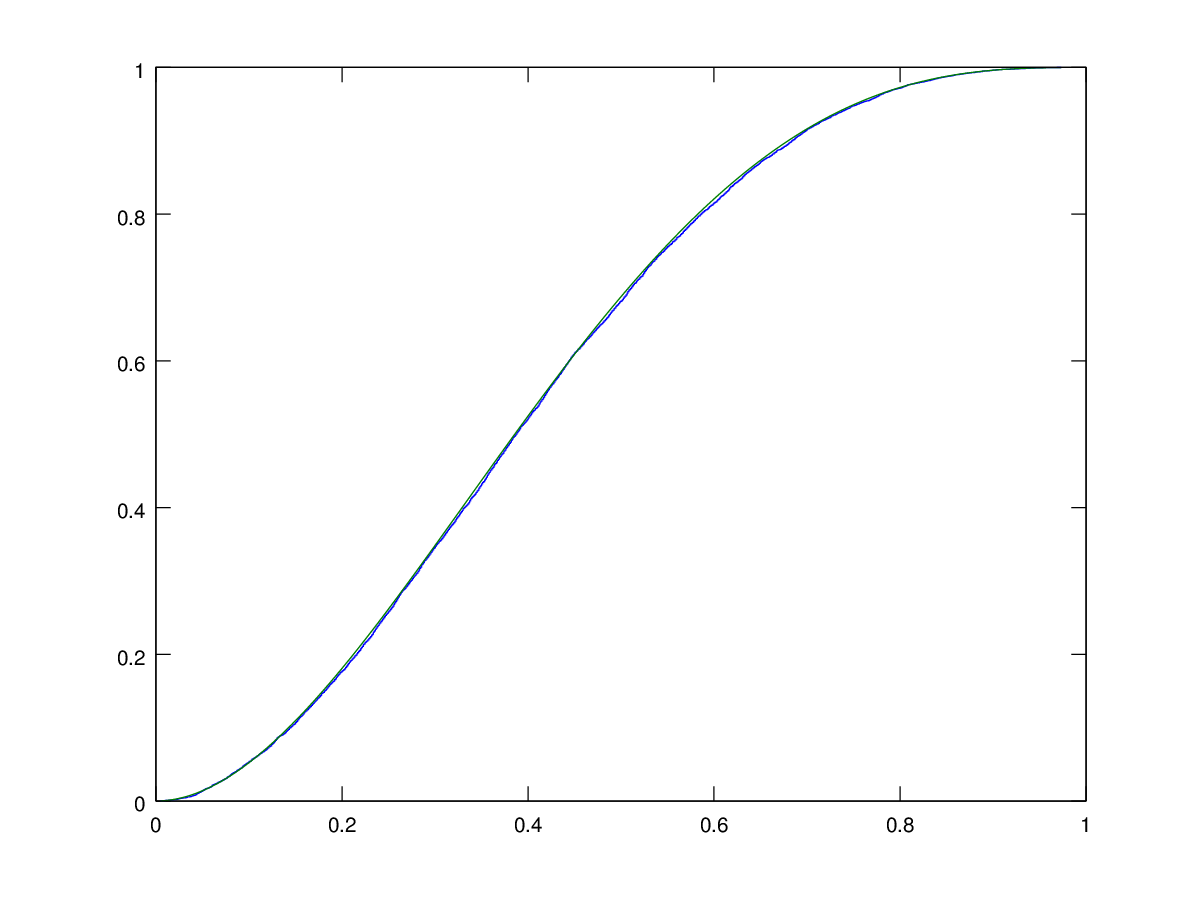
\includegraphics[width=8cm]{tarea3/problema3_4/poylaBeta.PNG}\pn
    Gr\'afica del histagrama de los radios ``finales'' de \texttt{10000} iteraciones del proceso 
	de urnas de P\'oyla (azul). En contraste con una distribución Beta (verde).\pn
\end{center}

En clase se demostró que los radios esperados tenían distribución Beta con los parámetros 
ya mencionados. En la gráfica se puede apreciar el parecido del resultado experimental con el teórico.\pn

P.S. \texttt{tic}, \texttt{toc} son funciones de octave para medir el tiempo de ejecución. En este caso
la ejecución duró cerca de un minuto. Lo cual era de esperarse, se realizaron poco más de \texttt{120,000,000} operaciones
y además, construir un gráfico con una retícula de \texttt{10000} puntos también es un proceso computacionalmente caro.
    \newpage

    \subsection{Inciso (ii)} \label{problema3_4:inciso2}
    \emph{
    Ejecute y explique la funci\'on del siguiente c\'odigo en Octave. 
    Incluya una gr\'afica en la que la longitud de la variable k sea mayor a 1000. 
    (Puede modificar el programa...) En la gr\'afica observara un esbozo de la 
    trayectoria de un proceso de ramificaci\'on continuo (en una escala distinta...).
    \texttt{
        \lstinputlisting[caption=]{tarea3/problema3_4/binaryGW.R}
    }
}

\afterstatement\pn

El código simula un proceso de Galton-Watson.\pn

\texttt{k = [10]} significa que al inicio habrá 10 individuos.\pn

\texttt{aux} es la última población obtenida. \texttt{binornd(aux, .5)} es una instrucción de Octave en la que
de un conjunto de \texttt{aux} elementos, escoge a cada uno con probabilidad \texttt{.5}. El resultado
es el número de elementos seleccionados. Multiplicar esto por \texttt{2} se puede interpretar como que
antes de morir, cada individuo seleccionado tiene dos hijos.\pn

\texttt{k = [k; 2*binornd(aux, .5)]} está agregando al vector \texttt{k} una nueva entrada. La entrada,
es la nueva población, resultante de que cada individuo seleccionado tiene dos hijos antes de morir y cada
elemento no seleccionado muere sin tener decendientes.\pn
 
A continuación, una gráfica con una ejecución de este algoritmo comenzando con \texttt{10} individuos
y terminando con \texttt{0} individuos después de un poco más de \texttt{12000} iteraciones.

\begin{center}
    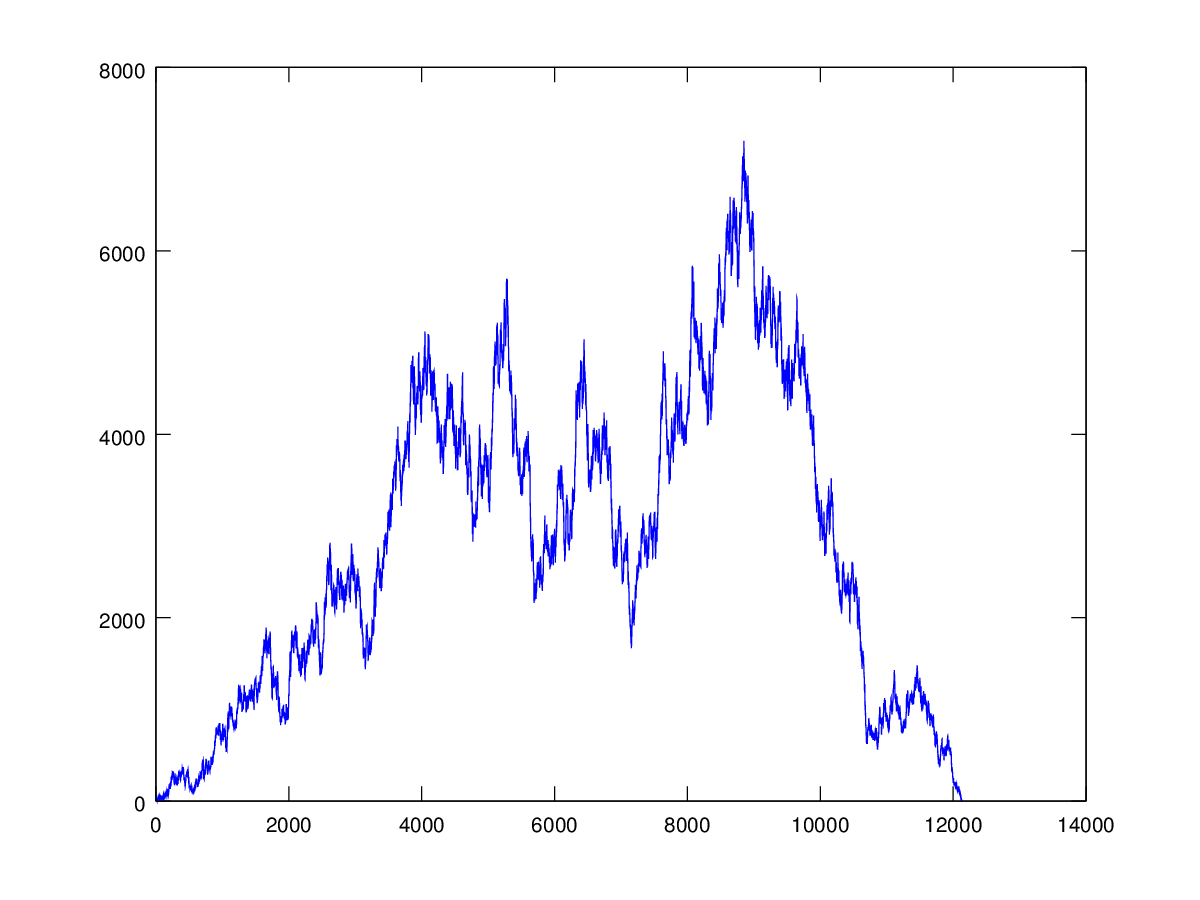
\includegraphics[width=8cm]{tarea3/problema3_4/galtonWatson.PNG}
    
    Gr\'afica de una ejecuci\'on del proceso de extinci\'on de Galton-Watson 
    Par\'ametros:\par
    10 individuos\par 
    La probabilidad de que un individuo tenga $2$ hijos es $\frac{1}{2}$\par
    La probabilidad de que un individuo tenga $0$ hijos es $\frac{1}{2}$.\pn
\end{center}

La esperanza de número de decendientes que tiene un individuo, es \texttt{1}. Es decir,
este proceso de Galton-Watson es crítico. En clase se demostró que los procesos Galton-Watson
críticos se extinguen con probabilidad \texttt{1}. La gráfica arriba mostrada es de una corrida
del algoritmo que más iteraciones duró antes de extinguirse, el algoritmo, se corrió
\texttt{200,000} veces y, en todos los casos se extingió la población. Esto es consistente con
con el resultado teórico (en todos los casos, de un conjunto de \texttt{200,000}, la población se extinguió).\pn

A continuación, una gráfica resultante del mismo algoritmo, pero con una población inicial de \texttt{1000} individuos.
que se extingue después de \texttt{20,000} iteraciones. Cabe mencionar que esta corrida fue más ``suertuda'' que la
representada en la gráfica anterior. Muchas de las corridas del algoritmo sin modificar superaron una población de
\texttt{1000} individuos en algún momento y después de eso, nunca duraron tanto como este otro.

\begin{center}
    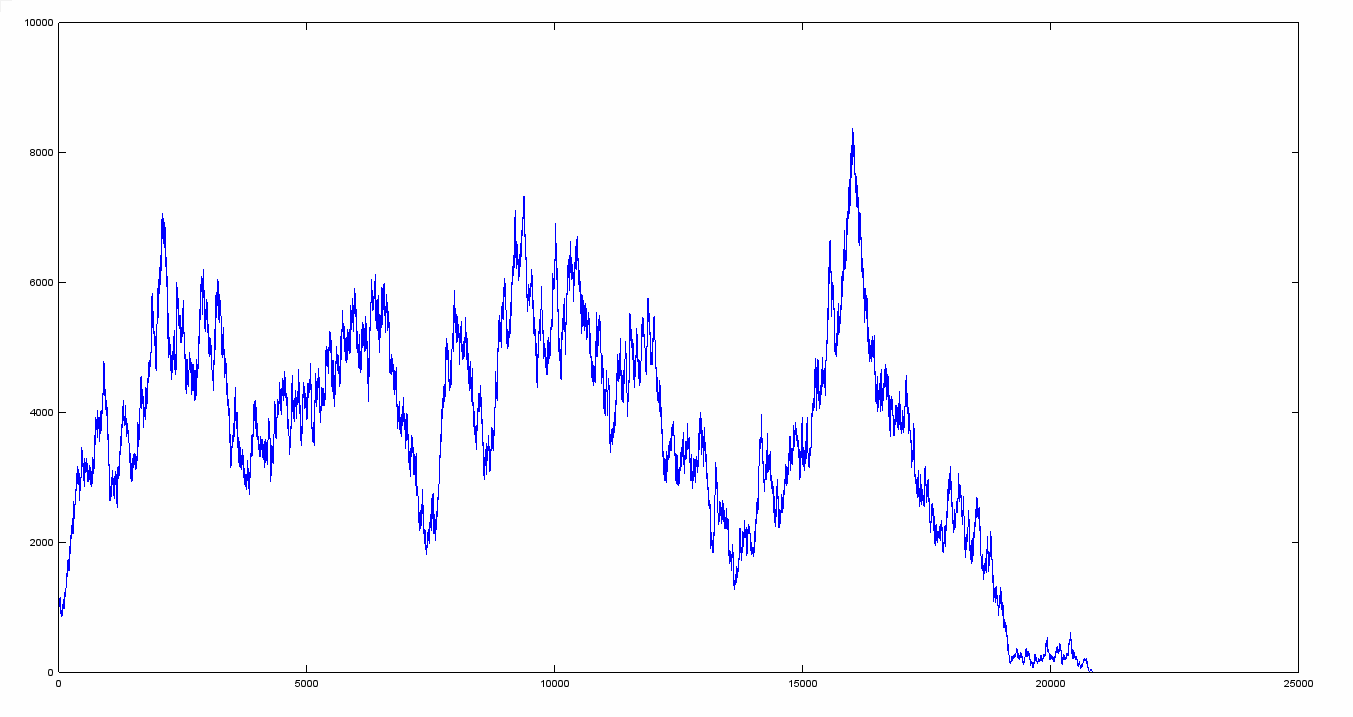
\includegraphics[width=12cm]{tarea3/problema3_4/galtonWatsonEmpezandoEn1000.PNG}
    
    Gr\'afica de una ejecuci\'on del proceso de extinci\'on de Galton-Watson 
    Par\'ametros:\par 
    1000 individuos iniciales \par
    La probabilidad de que un individuo tenga $2$ hijos es $\frac{1}{2}$ \par
    La probabilidad de que un individuo tenga $0$ hijos es $\frac{1}{2}$.\pn
\end{center}

P.S. El algoritmo modificado se incluye bajo el nombre de \par
\texttt{BinaryGWModificado.R}. (Incluí un candado para que el algoritmo terminara si 
superaba un millón de iteraciones, nunca se alcanzó dicho límite).
\end{proof}        
        \nqed
            
    \part{Tarea 4}
        \section{Problema 4.1}  \label{problema4_1}
\begin{problema}
	Sean $\F_1,\F_2,\ldots $ y $\G$ sub\sa s de $\F$. 
	Decimos que $\F_1,\F_2,\ldots$ son condicionalmente independientes dada $\G$ si para 
	cualquier $H_i$ que sea $\F_i$ medible y acotada se tiene que
	
	\begin{esn}
		\espc{H_1\cdots H_n}{\G}=\espc{H_1}{\G}\cdots \espc{H_n}{\G}.
	\end{esn}
	
	\begin{enumerate}
		\item[(i)]	[\ref{problema4_1:inciso1}]
			?`Qu\'e quiere decir la independencia condicional cuando $\G=\set{\oo,\emptyset}$?
			\pn

		\item[(ii)] 	[\ref{problema4_1:inciso2}]
			Pruebe que $\F_1$ y $\F_2$ son condicionalmente independientes dada $\G$ 
			(denotado $\condind{\F_1}{\F_2}{\G}$) si y s\'olo si para 
			cualquier $H$ que sea $\F_1$-medible y acotada se tiene que
			\begin{esn}
				\espc{H}{\F_2,\G}=\espc{H}{\G}.
			\end{esn}

		\item[(iii)]	[\ref{problema4_1:inciso3}]
			Pruebe que $\F_1,\F_2,\ldots, $ son condicionalmente independientes dada 
			$\G$ si y s\'olo si para cada $n\geq 1$, $\F_{n+1}$ es condicionalmente 
			independiente de $\F_1,\ldots, \F_n$ dada $\G$. 
	\end{enumerate}

	\defin{Categor\'ias: } Esperanza condicional, Independencia condicional.
\end{problema}

\begin{proof}
    \subsection{Inciso (i)} \label{problema4_1:inciso1}
    \emph{
	?`Qu\'e quiere decir la independencia condicional cuando $\G=\set{\oo,\emptyset}$?
}
    \newpage

    \subsection{Inciso (ii)} \label{problema4_1:inciso2}
    \emph{
		Pruebe que $F_1$ y $\F_2$ son condicionalmente independientes dada $\G$ 
		(denotado $\condind{\F_1}{\F_2}{\G}$) si y s\'olo si para 
		cualquier $H$ que sea $\F_1$-medible y acotada se tiene que
		\begin{esn}
			\espc{H}{\F_2,\G}=\espc{H}{\G}.
		\end{esn}
}
    \newpage

    \subsection{Inciso (iii)} \label{problema4_1:inciso3}
    \emph{
	Pruebe que $\F_1,\F_2,\ldots, $ son condicionalmente independientes dada 
	$\G$ si y s\'olo si para cada $n\geq 1$, $\F_{n+1}$ es condicionalmente 
	independiente de $\F_1,\ldots, \F_n$ dada $\G$. 
}

\afterstatement\par\null

Primero demostraremos la suficiencia. Para ello emplearemos el ejercicio anterior.
Sean $H_1, \dots, H_{n+1}$ variables aleatorias $\F_1, \dots, \F_{n+1}$-medibles (respectivamente) 
y acotadas.\par\null

Sea $P = \{ A : A = F_1 \cap \dots \cap \F_n \cap \G \text{ donde } F_i \in \F_i \text{ y } G \in \G \}$,
Es claro que $P \subset \sigma(\F_1, \dots, \F_n, \G)$. También es fácil ver que no es vacía ($\Omega$ es uno de sus elementos), 
y que es cerrada bajo intersecciones finitas. En otras palabras $C$ es un $\pi$-sistema. Además, justo
igual que antes, tenemos que $\sigma(P) = \sigma(\F_1, \dots, \F_n, \G)$.\par\null

Ahora sea $D = \{ A \in \sigma(\F_1, \dots, \F_n, \G) : \E(H_{n+1} \indic_A) = \E(\E(H_{n+1} | \G) \indic_A) \}$




\end{proof}
\newpage

\section{Problema 4.2}  \label{problema4_2}
\begin{problema}
	Sea $\mu$ una distribuci\'on de progenie y defina $\tilde \mu_j=\mu_{j+1}$. 
	Sea $S=\paren{S_n}$ una caminata aleatoria con distribuci\'on de salto $\tilde\mu$. 
	Sea $k$ un entero no-negativo y defina recursivamente

	\begin{esn}
		Z_0=k=C_0,\quad Z_{n+1}=k+S_{C_n} \quad \text{y} \quad C_{n+1}=C_n+Z_{n+1}.
	\end{esn}

	\begin{enumerate}
		\item[(i)]		[\ref{problema4_2:inciso1}]
			Pruebe que $Z_n\geq 0$ para toda $n$ y que si $Z_n=0$ entonces $Z_{n+1}=0$.\par\null
		
		\item[(ii)]		[\ref{problema4_2:inciso2}]
			Pruebe que $C_n$ es un tiempo de paro para la filtraci\'on can\'onica asociada a $S$.\par\null
		
		\item[(iii)] 	[\ref{problema4_2:inciso3}]
			Pruebe que $Z$ es un proceso de Galton-Watson con ley de progenie $\mu$.\par\null
		
		\item[(iv)]		[\ref{problema4_2:inciso4}] 
			Pruebe que si $S$ alcanza $-1$ entonces existe $n$ tal que $Z_n=0$. Deduzca que si la media de $\mu$ es $1$ entonces $Z$ se extingue. (Sugerencia: utilice un ejercicio anterior sobre martingalas con saltos acotados hacia abajo.) 
	\end{enumerate}

	\defin{Categor\'ias: } Caminatas aleatorias, Procesos de Galton-Watson%, Propiedad de Markov fuerte.
\end{problema}

\begin{proof}
    \subsection{Inciso (i)} \label{problema4_2:inciso1}
    \emph{
    Pruebe que $Z_n\geq 0$ para toda $n$ y que si $Z_n=0$ entonces $Z_{n+1}=0$.
}

\afterstatement\pn

Sean $(\xi_i)_{i \in \N}$ v.a.i.i.d con distribución $\tilde\mu$ 
(es decir, $\mw(\xi_i = s) = \tilde\mu_s$ donde $-1 \leq s$).\pn

Es decir que podemos denotar a $S_n = \sum_{i \leq n} \xi_i$.\pn

Primero demostraremos que $Z_n \geq 0$. La demostración se hará por inducción sobre $n$.

\begin{itemize}
	\item 
        \textbf{Base De Inducción.}
        
        Para $n = 0$ tenemos $Z_0 = k \geq 0$.\pn
        
    \item
        \textbf{Hipótesis De Inducción.}
        
        Sea $n$ tal que $Z_i \geq 0$ para toda $i \leq n$.\pn
        
    \item
        \textbf{Paso Inductivo.}
        
        \begin{align} \label{problema4_2:descomposicion_de_Z_n+1}
            Z_{n+1}     &=  k + S_{C_n}                                                                             \\
                        &=  k + \sum_{i \leq C_n} \xi_i                                                             \\
                        &=  k + \sum_{i \leq C_{n-1} + Z_{n}} \xi_i                                                 \\
                        &=  k + \sum_{i \leq C_{n-1}} \xi_i + \sum_{C_{n-1} < i \leq  C_{n-1} + Z_{n}} \xi_i        \\
                        &=  k + S_{C_n-1} + \sum_{C_{n-1} < i \leq  C_{n-1} +Z_{n}} \xi_i                           \\
                        &=  Z_n + \sum_{C_{n-1} < i \leq  C_{n-1} + Z_{n}} \xi_i                                    \\                        
        \end{align}
        
        En la suma del lado derecho tenemos exáctamente $Z_n$ sumandos, y cada sumando es mayor o igual a $-1$. Entonces
        en el peor de los casos la suma de la derecha es igual a $-Z_n$. Es decir, 
        
        \begin{align}
            \sum_{C_{n-1} < i \leq  C_{n-1} + Z_{n}} \xi_i \geq -Z_n.
        \end{align}
        
        Y combinando estos resultados tenemos
        
        \begin{align}
            Z_{n+1} &=      Z_n + \sum_{C_{n-1} < i \leq  C_{n-1} + Z_{n}} \xi_i    \\
                    &\geq   Z_n - Z_n                                               \\
                    &=      0.
        \end{align}
        
        Y con esto termina la demostración.
\end{itemize}

Ahora demostraremos que si $Z_n = 0$, entonces $Z_{n+1} = 0$.\pn

Notemos los siguientes hechos. 
\begin{itemize}
	\item 
        $Z_n = k + S_{C_{n-1}} = 0$ implica que $S_{C_{n-1}} = -k$.
    
    \item
        $C_n = C_{n-1} + Z_n = C_{n-1}$.
\end{itemize}

Con esto presente, basta recordar la definición de $Z_{n+1}$:

\begin{align}
    Z_{n+1} &=  k   +   S_{C_n}         \\
            &=  k   +   S_{C_{n-1}}     \\
            &=  k   -   k               \\
            &=  0.
\end{align}

Que era lo que buscábamos demostrar.
    \newpage

    \subsection{Inciso (ii)} \label{problema4_2:inciso2}
    \emph{
	Pruebe que $C_n$ es un tiempo de paro para la filtraci\'on can\'onica asociada a $S$.
}

\afterstatement\pn

Sea $(\F_n)_{n \in \N}$ la filtración canónica asociada a $(S_n)_{n \in \N}$.
Tenemos que demostrar que para $m \in \Z$, $\{ C_n = m \} \in \F_m$.\pn

Usemos la definición de $C_n$ para descomponerlo, 

\begin{align}\label{problema4_2:descomposicion_de_C_n}
    C_n &=  C_{n-1} + Z_n                   \\
        &=  C_{n-2} + Z_{n-1} + Z_n         \\
        &\vdots                             \\
        &= k + \sum_{1 \leq i \leq n} Z_i   
\end{align}

Ahora, recordando que $0 \leq Z_i$, tenemos que $k \leq C_n$, es decir que
$\{ C_n < k\} = \emptyset$, en particular, si $m < k$, $\{C_n = m\} = \emptyset \in \F_m$.\pn

Supongamos entonces que $k \leq m$. De nuevo gracias a que $0 \leq Z_i$, tenemos que la sucesión $(C_i)_{i \in \N}$
es creciente. Entonces, dentro del conjunto $\{ C_n = m\}$ tenemos que $C_i \leq m$ para $i \leq n$. Y por lo tanto,
dentro del conjunto $\{ C_n = m\}$, $S_{C_i}$ es $\F_m$-medible (donde dentro del conjunto se debería interpretar como
al intesectar con dicho conjunto, las preimagenes de $S_{C_i}$ pertenecen a $\F_m$).\pn

Entonces $Z_i = S_{C_{i-1}}$ también resulta ser $\F_m$-medible (dentro de $\{ C_n = m \}$ y por lo tanto. Entonces nos
basta con descomponer $\{ C_n = m \}$ en conjuntos que sean $\F_m$-medibles usando lo que hemos demostrado ahora.
Utilizando \eqref{problema4_2:descomposicion_de_C_n} tenemos que

\begin{align}
    \{ C_n = m \}   &=  \bigg\{ k + \sum_{1 \leq i \leq n} Z_i  = m \bigg\}.                         
\end{align}

Y por todo lo anteriormente dicho, el lado derecho de la igualdad resulta ser $\F_m$-medible.

    \newpage

    \subsection{Inciso (iii)} \label{problema4_2:inciso3}
    \emph{
	Pruebe que $Z$ es un proceso de Galton-Watson con ley de progenie $\mu$.
}

\afterstatement\par\null

Tenemos que encontrar variables $\zeta_{i,n}$ con distribución $\mu$ tales que

\begin{align}
    Z_{n+1} =   \sum_{1 \leq i \leq Z_n} \zeta_{i,n}. \label{problema4_2:expresion_Galton-Watson}
\end{align}

Sean $\xi_{i}$ con $-1 \leq i$ definidas como en el primer inciso de este ejercicio [\ref{problema4_2:inciso1}],
estas estaban definidas bajo una distribución $\tilde\mu$ que era exactamente igual a $\mu$ pero desfasada por $-1$.
Es decir $\tilde\mu_{-1} = \mu_{0}, \tilde\mu_{0} = \mu_{1}, \dots, \tilde\mu_{j} = \mu_{j+1}$. Entonces, 
$\xi_{i} + 1$ tendrá distribución $\mu$.\par\null

Ya teníamos una descomposición útil de $Z_{n+1}$ en \eqref{problema4_2:descomposicion_de_Z_n+1}. La reescribiremos cambiando $\xi_{i}$
por $\xi_{i} + 1 - 1$.

\begin{align}
    Z_{n+1} &=  Z_n + \paren{\sum_{C_{n-1} < i \leq  C_{n-1} + Z_{n}} \xi_i}                \\
            &=  Z_n + \paren{\sum_{C_{n-1} < i \leq  C_{n-1} + Z_{n}} (\xi_i + 1 - 1)}      \\
            &=  Z_n + \paren{\sum_{C_{n-1} < i \leq  C_{n-1} + Z_{n}} (\xi_i + 1)} - Z_n    \\
            &=  \paren{\sum_{C_{n-1} < i \leq  C_{n-1} + Z_{n}} (\xi_i + 1)}                
\end{align}

Ahora que tenemos a $Z_{n}$ expresado como suma de variables con distribución $\mu$, bastará reescribirlo de manera que
tenga la forma \eqref{problema4_2:expresion_Galton-Watson}.\par\null

Definamos entonces $\zeta_{i, n} = \xi_{C_{n-1} + 1$, y entonces

\begin{align}
    Z_{n+1} &=  \paren{\sum_{C_{n-1} < i \leq  C_{n-1} + Z_{n}} (\xi_i + 1)}    \\
            &=  \paren{\sum_{1 \leq i \leq Z_{n}} (\zeta_{i, n})}.
\end{align}

Y con esto hemos demostrado que $Z$ es un proceso Galton-Watson con distribución de progenie $\mu$ y, como $Z_0 = k$, se trata
de un proceso Galton-Watson con población inicial $k$.
	\newpage
	
    \subsection{Inciso (iv)} \label{problema4_2:inciso4}
    \emph{
    Pruebe que si $S$ alcanza $-1$ entonces existe $n$ tal que $Z_n=0$. 
    Deduzca que si la media de $\mu$ es $1$ entonces $Z$ se extingue. 
    (Sugerencia: utilice un ejercicio anterior sobre martingalas con saltos acotados hacia abajo.) 
}

\afterstatement\par\null

Suponiendo que la media de $\mu$ es $1$, significa que $\E(\xi_i + 1) = 1$ y por lo tanto $\E(\xi_i) = 0$.\par\null

Esto convierte a $(S_n)_{n \in \N}$ en una caminata aleatoria no trivial y centrada (la media de sus saltos es 0).
Por lo dicho en [\ref{problema3_2}] tenemos que es una caminata que oscila y por lo tanto $\liminf S_n = -\infty$.\par\null

Esto quiere decir que existe un $n$ tal que $S_{C_{n}} = -k$ y entonces 
$Z_{n + 1} = k + S_{C_{n}} = k - k = 0$. Lo cual se traduce en que la población se extinge casi seguramente.\par\null
\end{proof}
\newpage

\section{Problema 4.3}  \label{problema4_3}
\begin{problema}
	El objetivo de este ejercicio es ver ejemplos de cadenas de Markov $X$ y de funciones $f$ tales que 
	$\imf{f}{X}=\paren{\imf{f}{X_n},n\in\na}$ sean o no cadenas de Markov.
	
	\begin{enumerate}
	\item[(i)]	[\ref{problema4_3:inciso1}]
		Considere el hipercubo $n$-dimensional $E=\set{0,1}^n$. A $E$ lo pensaremos como la composici\'on 
		de la primera de dos urnas que tienen en total $n$ bolas etiquetadas del $1$ al $n$. 
		Si $x=\paren{x_1,\ldots, x_n}\in E$, interpretaremos $x_i=1$ como que la bola $i$ est\'a en la urna $1$. 
		Considere el siguiente experimento aleatorio: inicialmente la composici\'on de las urnas est\'a dada por 
		$x$ y a cada instante de tiempo escogemos una bola al azar y la cambiamos de urna. 
		Modele esta situaci\'on por medio de una cadena de Markov $X$ en $E$. Sea $\fun{f}{E}{\set{0,\ldots, n}}$ 
		dada por $\imf{f}{x}=\sum_i x_i$. Pruebe que $\imf{f}{X}=\paren{\imf{f}{X_n},n\in\na}$ es una cadena de 
		Markov cuya matriz de transici\'on determinar\'a.

	\item[(ii)]	[\ref{problema4_3:inciso2}]
		Sea $\paren{S_n}_{n\in\na}$ una cadena de Markov con espacio de estados $\z$ y matriz de transici\'on
		\begin{esn}
		P_{i,i+1}=p\quad P_{i,i-1}=1-p
		\end{esn}	
		donde $p\in [0,1]$. D\'e una condici\'on necesaria y suficiente para que $\paren{\abs{S_n},n\in\na}$ 
		sea una cadena de Markov.
	\end{enumerate}

\defin{Categor\'ias:} proyecciones de cadenas de Markov
\end{problema}

\begin{proof}
    \subsection{Inciso (i)} \label{problema4_3:inciso1}
    \emph{
	Considere el hipercubo $n$-dimensional $E=\set{0,1}^n$. A $E$ lo pensaremos como la composici\'on 
	de la primera de dos urnas que tienen en total $n$ bolas etiquetadas del $1$ al $n$. 
	Si $x=\paren{x_1,\ldots, x_n}\in E$, interpretaremos $x_i=1$ como que la bola $i$ est\'a en la urna $1$. 
	Considere el siguiente experimento aleatorio: inicialmente la composici\'on de las urnas est\'a dada por 
	$x$ y a cada instante de tiempo escogemos una bola al azar y la cambiamos de urna. 
	Modele esta situaci\'on por medio de una cadena de Markov $X$ en $E$. Sea $\fun{f}{E}{\set{0,\ldots, n}}$ 
	dada por $\imf{f}{x}=\sum_i x_i$. Pruebe que $\imf{f}{X}=\paren{\imf{f}{X_n},n\in\na}$ es una cadena de 
	Markov cuya matriz de transici\'on determinar\'a.
}
\afterstatement\pn

Sean $i,j \in E$. Definamos las siguientes entradas de una matriz de transición:

\begin{align}
        p_{i,j} &=   
                    \begin{cases}
                        \frac{1}{n},    &       \|i-j\| = 1 \comment{donde $\|\cdot\|$ es la norma euclidiana}  \\
                        0,              &       \text{en cualquier otro caso}
                    \end{cases}
\end{align}

Dado $i \in E$, sólo existen $n$ vectores que distan exáctamente $1$ de $i$. Entonces 
$\sum_{j \in E} \frac{1}{n} = n \frac{1}{n} = 1$ y nuestra matriz sí es de transición.\pn

Ya que nuestro proceso está restringido a comenzar en $x$, nuestra distribución inicial
será $\lambda = (\lambda_i : i \in E)$ tal que $\lambda_x = 1$ y $\lambda_i = 0$ si $i \not= x$.\pn

Es fácil notar que la evolución del proceso depende únicamente del presente. Para llegar a una configuración
de bolas en particular, únicamente es importante en qué configuración se encuentra actualmente.\pn

Dado que tenemos una matriz de transición y una distribución inicial bien definidas, existe una cadena de
Markov $X$ con dichas matriz de transcición y distribución inicial que describen la evolución del proceso.\pn

El proceso $(f(X_n))_{n \in N}$ es el proceso que cuenta la cantidad de bolas en la urna $1$ que equivale al proceso
de Ehrenfest, el cual es una cadena de Markov y las entradas de su matriz de transición están dadas por

\begin{align}
        p_{i,j}     &=  
                        \begin{cases}
                            \frac{n-i}{n},  &   j=i+1   \\
                            \frac{i}{n},    &   j=i-1   \\
                            0,              &   \text{en cualquier otro caso.}
                        \end{cases}
\end{align}
    \newpage

    \subsection{Inciso (ii)} \label{problema4_3:inciso2}
    \emph{
	Sea $\paren{S_n}_{n\in\na}$ una cadena de Markov con espacio de estados $\z$ y matriz de transici\'on
	\begin{esn}
	P_{i,i+1}=p\quad P_{i,i-1}=1-p
	\end{esn}	
	donde $p\in [0,1]$. D\'e una condici\'on necesaria y suficiente para que $\paren{\abs{S_n},n\in\na}$ 
	sea una cadena de Markov.
}

Tenemos que $\abs{S_{n - 1} - S_n} = 1$ con probabilidad $1$. Esto significa, los saltos del proceso siempre son
de tamaño $1$. Esto significa que, la paridad de un estado al siguiente siempre cambia con probabilidad $1$. En
otras palabras, la paridad se preserva después de una cantidad par de pasos.\pn

Es decir que si $r_1, r_2 \in \Z$ entonces:
\begin{align}
        \mw(S_{2n + n_0} = r_2 | S_{n_0} = r_1 ) =
                                                    \begin{cases}
                                                        1,  \text{si $2$ divide a $r_1 - r_2$} \\
                                                        0,  \text{si $2$ no divide a $r_1 - r_2$} 
                                                    \end{cases}
\end{align}

La paridad se preserva bajo valor absoluto, así que lo mismo ocurre en el caso de $\abs{S_n}$
\end{proof}
\newpage

\section{Problema 4.4}  \label{problema4_4}
\begin{problema}
Sean $\p$ y $\q$ dos medidas de probabilidad en el espacio can\'onico $E^\na$ para sucesiones con valores en un conjunto a lo m\'as numerable $E$. Decimos que $\q$ es \defin{localmente absolutamente continua} respecto de $\p$ si para cada $n\in\na$, $\q|_{\F_n}\ll\p|_{\F_n}$. Sea\begin{esn}
D_n=\frac{d \q|_{\F_n}}{d \p|_{\F_n}}.
\end{esn}
\begin{enumerate}
\item Pruebe que $D$ es una martingala bajo $\p$. Pruebe que si $D$ es uniformemente integrable entonces $\q\ll\p$. 
\item Pruebe que si $T$ es un tiempo de paro finito entonces $\q|_{\F_T}\ll\p|_{\F_T}$. 
\item Sea $\p^p$ la distribuci\'on de una caminata aleatoria simple que comienza en $0$ y va de $k$ a $k+1$ con probabilidad $p$, donde $p\in (0,1)$. Pruebe que $\p^p$ es localmente absolutamente continua respecto de $\p^{1/2}$ y encuentre la martingala $D_n$ asociada.
\item Para $a,b>0$, sea $T=\min\set{n\in\na: X_n\in \set{-a,b}}$. Pruebe que $T$ y $X_T$ son independientes bajo $\p^{1/2}$. Al utilizar la continuidad absoluta local, pruebe que $T$ y $X_T$ tambi\'en son independientes bajo $\p^p$. Utilice alguna martingala de ejercicios anteriores para calcular $\esp{T^2}$. 
\end{enumerate}

\defin{Categor\'ias: }Cambio de medida, Caminata aleatoria simple.
\end{problema}        
        \nqed    
    
    \part{Tarea 5}
        \section{Problema 5.1}
\begin{problema}
Sea $N$ un proceso Poisson de par\'ametro $\lambda$ y sea $T_n$ el tiempo de su en\'esimo salto. 
\begin{enumerate}
\item Pruebe que condicionalmente a $T_2$, $T_1$ es uniforme en $[0,T_2]$. 
\item Pruebe que si $W_1$ y $W_2$  son  exponenciales de par\'ametro $\lambda$  independientes entre si y de una variable uniforme $U$, entonces $U\paren{W_1+W_2}$ es una variable aleatoria exponencial de par\'ametro $\lambda$. 
\item Conjeture c\'omo se  generaliza lo anterior con $T_n$ y $T_1$.
\item Escriba dos programas en Octave que simulen al proceso de Poisson de par\'ametro $\lambda$ en el intervalo $[0,1]$. En uno utilizar\'a s\'olo variables exponenciales y en el otro puede utilizar una variable Poisson.
\end{enumerate}
\end{problema}

\newpage

\section{Problema 5.2}
\begin{problema}
%Simulaci\'on de un proceso Poisson puntual... subordinador...
    Sea $\Xi$ una medida de Poisson aleatoria en $(0,\infty)\times (0,\infty)$ cuya 
    medida de intensidad $\nu$ est\'a dada por $\imf{\nu}{ds,dx}=\indi{x>0}C/x^{1+\alpha}\, ds\,dx$. 
    
    \begin{enumerate}
        \item Determine los valores de $\alpha$ para los cuales $\int 1\wedge x\,\imf{\nu}{dx}<\infty$. 
    \end{enumerate}
    
    Nos restringimos ahora a valores de $\alpha$ para los cuales la integral anterior sea finita. Sean $\imf{f_t}{s,x}=\indi{s\leq t}x$ y $X_t=\Xi f_t$. 
    
    \begin{enumerate}[resume]
        \item Determine los valores  de $\alpha$ para los cuales $X_t<\infty$ para toda $t\geq 0$ casi seguramente.
    \end{enumerate}

    Nos restringiremos a dichos valores de $\alpha$. 
    
    \begin{enumerate}[resume]
        \item Calcule $\esp{e^{-\lambda X_t}}$ y pruebe que $X_{t}$ tiene la misma distribuci\'on que $t^{1/\alpha}X_1$. 
        \item Diga por qu\'e el siguiente c\'odigo en Octave simula la trayectoria aproximada del proceso $X$ en el intervalo $[0,1]$.
        \lstinputlisting{tarea5/problema5_2/SuborEst.m}
    \end{enumerate}
\end{problema}
\newpage

\section{Problema 5.3}
\begin{problema}.\pn
	
	\begin{enumerate}
		\item[(i)]		[\ref{problema5_3:inciso1}]
			Pruebe que si $X$ tiene incrementos independientes entonces el proceso $X^t$ dado por $X^t_s=X_{t+s}-X_t$ 
			es independiente de $\F^X_t=\sag{X_s:s\geq 0}$.

		\item[(ii)]		[\ref{problema5_3:inciso2}]
			Calcular la esperanza y varianza del proceso de Poisson y de Poisson compuesto (en t\'erminos de 
			la intensidad y la distribuci\'on de salto). Probar que si $X$ es proceso Poisson compuesto con salto $\xi_i$
			\begin{esn}
				\esp{e^{iu X_t}}=e^{-\lambda t\paren{1-\imf{\psi}{u}}}\quad\text{donde}\quad \imf{\psi}{u}=\esp{e^{iu \xi_1}}. 
			\end{esn}
	\end{enumerate}\pn
		Sea $N$ un proceso de L\'evy tal que $N_t$ tiene distribuci\'on de par\'ametro $\lambda t$. 

	\begin{enumerate}[resume]
		\item[(iii)]	[\ref{problema5_3:inciso3}] 
			Pruebe que casi seguramente las trayectorias de $N$ son no-decrecientes.
		\item[(iv)]		[\ref{problema5_3:inciso4}] 
			Sea $\Xi$ la \'unica medida en $\mc{B}_{\re_+}$ tal que $\imf{\Xi}{[0,t]}=N_t$. Pruebe que 
			$\Xi$ es una medida de Poisson aleatoria de intensidad $\lambda \cdot\leb$.
		\item[(v)]		[\ref{problema5_3:inciso5}]
			Concluya que $N$ es un proceso de Poisson de intensidad $\lambda$. 
	\end{enumerate}
\end{problema}

\begin{proof}
    \subsection{Inciso (i)}	    \label{problema5_3:inciso1}
	\emph{
	Pruebe que si $X$ tiene incrementos independientes entonces el proceso $X^t$ dado por $X^t_s=X_{t+s}-X_t$ 
	es independiente de $\F^X_t=\sag{X_s : s \leq t}$.
}

\afterstatement\pn

Recordemos que tener incrementos independientes significa que siempre que $0 \leq r_1 < r_2 < r_3 < \dots < r_m$ 
se tiene que $X_{r_1} - X_{r_2}, X_{r_2} - X_{r_3}, \dots, X_{r_m} - X_{t_{m-1}}$ son variables aleatorias 
independientes.\pn

Veamos quien es la $\sigma$-álgebra generada por los incrementos de $X$ hasta $t$. En otras palabaras, 
la $\sigma$-álgebra generada por conjuntos de la forma

\begin{align}
    \bigcap_{1 \leq i \leq n} \{ X_{s_i} - X_{s_{i-1}} \in B_i \} \label{problema5_3:sigma_algebra_de_incrementos}
\end{align}\pn

Donde $0 \leq s_1 < s_2 < \dots < s_n \leq t$, $B_i \in \B_\R$ y, por comodida de notación, $X_{s_{0}} = 0$.\pn 

Notemos primero que estos conjuntos son todos $\F_t^X$ medibles. También notemos que los conjuntos 
$\{ X_s \in B : B \in \B_\R \}$ con $0 \leq s \leq t$ también son de esta forma. Basta con escoger 
$s_1 = s$, $B_1 = B$ y $B_i = \R$ para $i \geq 2$.\pn

Lo que acabamos de mostrar es que la $\sigma$-álgebra generada por los conjuntos definidos en 
\eqref{problema5_3:sigma_algebra_de_incrementos} es igual a $\F_t^X$. Llamemos $P$ a la clase 
de los conjuntos de esta forma. Es fácil ver que $P$ es un $\pi$-sistema. Es no vacío ($\R$ y $\emptyset$ 
pertenecen a él) y es fácil ver que la intersección de dos de ellos está otra vez en $P$.\pn

Ahora analicemos a la $\sigma$-álgebra generada por los incrementos de $X^t$. Llamemos $P'$ a
la clase de los conjuntos de la forma

\begin{align}
    \bigcap_{1 \leq i \leq n} \{  X_{t + r_i} - X_{t + r_{i - 1}} \in B_i \}
\end{align}

Donde $0 \leq r_1 < r_2 < \dots < r_n$,  $B_i \in \B_\R$ y, por comodida de notación 
$r_0 = 0$. Otra vez, es fácil notar que $P'$ es un $pi$-sistema. Es no vacío ($\R$ y $\emptyset$ 
pertenecen a él) y es fácil ver que la intersección de dos de ellos está otra vez en $P'$.\pn

$P'$ en la forma que lo construimos, es el álgebra de los incrementos de $X^t$, por lo tanto, 
la $\sigma$-álgebra que genera es la $\sigma$-álgebra de los incrementos de $X^t$.\pn

La idea ahora es encontrar un sistema de Dynkin que contenga a $P$ y que sea independiente
de $P'$. De esta manera, utilizando el Lema de clases de Dynkin podemos extender la propieadad de ser
independiente de $P'$.\pn

Sea $C' \in P'$. Definimos
\begin{align}
    D_{C'} =   \{ S \in \sigma(P) : \P(S  \cap C') = \P(S) \P(C') \}.
\end{align}\pn

Veamos que $P \subset D_{C'}$. Para ello, sea $C \in P$ con
\begin{align}
     C  &=  \bigcap_{1 \leq i\leq n} \{ X_{s_i} - X_{s_{i-1}} \in B_i \}.
\end{align}\pn

Como $C' \in P$, entonces se puede escribir como
\begin{align}
    C'  &=  \bigcap_{1 \leq i' \leq n'} \{  X_{t + r_i'} - X_{t + r_{i' - 1}} \in B_i' \}
\end{align}

Entonces
\tiny               
\begin{align}
    &   \P(C \cap C')                                                                                                                                                                                                                                                   =   \\
    &   \P\left( \left[ \bigcap_{1 \leq i\leq n} \{ X_{s_i} - X_{s_{i-1}} \in B_i \} \right] \cap \left[ \bigcap_{1 \leq i' \leq n'} \{  X_{t + r_i'} - X_{t + r_{i' - 1}} \in B_i' \} \right] \right)                                                                  =   \\
    &   \P\left( \left[ \bigcap_{1 \leq i\leq n} \{ X_{s_i} - X_{s_{i-1}} \in B_i \} \right] \cap \{X_t - X_{s_n} \in \R\} \cap \left[ \bigcap_{1 \leq i' \leq n'} \{  X_{t + r_i'} - X_{t + r_{i' - 1}} \in B_i' \} \right] \right)                                    =   \\
    &   \comment{Se está intersectando con un conjunto que es igual a $\R$, por eso la igualdad se preserva}                                                                                                                                                                \\
    &   \P\left( \left[ \bigcap_{1 \leq i\leq n} \{ X_{s_i} - X_{s_{i-1}} \in B_i \} \right] \right) \cdot \P\left( \{X_t - X_{s_n} \in \R\} \right) \cdot \P\left(\left[ \bigcap_{1 \leq i' \leq n'} \{  X_{t + r_i'} - X_{t + r_{i' - 1}} \in B_i' \} \right] \right) =   \\
    &   \comment{Se utilizó la hipótesis de que $X$ tiene incrementos independientes}                                                                                                                                                                                       \\
    &   \P\left( \left[ \bigcap_{1 \leq i\leq n} \{ X_{s_i} - X_{s_{i-1}} \in B_i \} \right] \right) \cdot \P\left(\left[ \bigcap_{1 \leq i' \leq n'} \{  X_{t + r_i'} - X_{t + r_{i' - 1}} \in B_i' \} \right] \right)                                                 =   \\
    &   \comment{El termino que desapareció era la probabilidad del total, es decir $1$}                                                                                                                                                                                    \\
    &   \P(C) \P(C').
\end{align}\pn
\normalsize

Con esto hemos demostrado que $C \in D_{C'}$ y por lo tanto $P \subset D_{C'}$.

	\newpage
	
	\subsection{Inciso (ii)}	\label{problema5_3:inciso2}
	\emph{
	Calcular la esperanza y varianza del proceso de Poisson y de Poisson compuesto (en t\'erminos de 
	la intensidad y la distribuci\'on de salto). Probar que si $X$ es proceso Poisson compuesto con salto $\xi_i$
	\begin{esn}
		\esp{e^{iu X_t}}=e^{-\lambda t\paren{1-\imf{\psi}{u}}}\quad\text{donde}\quad \imf{\psi}{u}=\esp{e^{iu \xi_1}}. 
	\end{esn}
}

\afterstatement\pn

Sea $N_t$ un proceso de Poisson de intensidad $\lambda$. Es decir, que la distribución de $N_t$ tiene distribución de Poisson de parámetro
$\lambda t$. Entonces:

\begin{align}
    \E(N_t) &=  \sum_{i \in \N} i \P(N_t = i)                                                   \\
            &=  \sum_{i \in \N} i e^{- \lambda t} \frac{(\lambda t)^i}{i!}                      \\
            &=  e^{- \lambda t} \sum_{i \in \N} i \frac{(\lambda t)^i}{i!}                      \\
            &=  e^{- \lambda t} (\lambda t) \sum_{i \in \N} \frac{(\lambda t)^{i-1}}{(i-1)!}    \\
            &=  e^{- \lambda t} (\lambda t) e^{\lambda t}                                       \\
            &=  \lambda t.
\end{align}

Ahora
\begin{align}
    \E(N_t^2)   &=  \sum_{i \in \N} i^2 \P(N_t = i)                                                                                                                         \\
                &=  e^{- \lambda t} \sum_{i \in \N} i^2 \frac{(\lambda t)^i}{i!}                                                                                            \\
                &=  e^{- \lambda t} \sum_{i \in \N} i \frac{(\lambda t)^i}{(i-1)!}                                                                                          \\
                &=  e^{- \lambda t} (\lambda t) \sum_{i \in \N} i \frac{(\lambda t)^{i-1}}{(i-1)!}                                                                          \\
                &=  e^{- \lambda t} (\lambda t) \sum_{i \in \N} (i - 1 + 1) \frac{(\lambda t)^{i-1}}{(i-1)!}                                                                \\
                &=  e^{- \lambda t} (\lambda t) \left(\sum_{i \in \N} (i - 1) \frac{(\lambda t)^{i-1}}{(i-1)!} + \sum_{i \in \N} \frac{(\lambda t)^{i-1}}{(i-1)!} \right)   \\                
                &=  e^{- \lambda t} (\lambda t) \left(\sum_{i \in \N} (i - 1) \frac{(\lambda t)^{i-1}}{(i-1)!} + e^{\lambda t} \right)                                      \\                
                &=  \left((\lambda t) e^{- \lambda t} \sum_{i \in \N} (i - 1) \frac{(\lambda t)^{i-1}}{(i-1)!} + e^{- \lambda t} (\lambda t) e^{\lambda t} \right)          \\                                      \\                
                &=  (\lambda t) \E(N_t) +  (\lambda t)                                                                                                                      \\                
                &=  (\lambda t)^2 +  (\lambda t).
\end{align}

Por lo tanto
\begin{align}
    Var(N_t)    &=  \E(N_t^2) - \E(N_t)^2                           \\
                &=  (\lambda t)^2 +  (\lambda t) - (\lambda t)^2    \\
                &=  (\lambda t).
\end{align}

Sea ahora $X$ un proceso de Poisson compuesto. Es decir
\begin{align}
    X_t     &=  \sum_{i \leq N_t} \xi_i.
\end{align}\pn

Con $\xi_i$ variables aleatorias independientes, idénticamente distribuidas e independientes del proceso de Poisson $N_t$.
Entonces 
\begin{align}
    \E(X_t)     &=  \E\left( \sum_{i \leq N_t} \xi_i \right)                                    \\
                &=  \E\left( \sum_{i \in \N} \xi_i \indic_{\{ T_i \leq t\}} \right)             \\
                &=  \left( \sum_{i \in \N} \E(\xi_i \indic_{\{ T_i \leq t\}}) \right)           \\
                &\comment{por teorema de la convergencia monótona}                              \\
                &=  \left( \sum_{i \in \N} \E(\xi_i) \E(\indic_{\{ T_i \leq t\}}) \right)       \\
                &\comment{por independencia de las $\xi$ del proceso de Poisson}                \\
                &=  \left( \sum_{i \in \N} \E(\xi_1) \E(\indic_{\{ T_i \leq t\}}) \right)       \\
                &\comment{por que las $\xi$ son idénticamente distribuidas}                     \\
                &=  \E(\xi_1) \left( \sum_{i \in \N} \E(\indic_{\{ T_i \leq t\}}) \right)       \\
                &=  \E(\xi_1) \E(N_t)                                                           \\
                &=  \E(\xi_1) (\lambda t).                                                        \\
\end{align}\pn

[ahora más cuentas]. 
\begin{align}
    \E(X_t^2)   &=  \E(\E(X_t^2 \bigg| N_t))                                                                                                                                \\
                &=  \E\left(\E\left[ \left(\sum_{i \leq N_t} \xi_i \right)^2 \bigg| N_t\right] \right)                                                                      \\
                &=  \E\left(\sum_{j \in \N} \E\left[ \left(\sum_{i \leq N_t} \xi_i \right)^2 \bigg| N_t = j\right] \indic_{\{ N_t = j\}} \right)                            \\
                &=  \E\left(\sum_{j \in \N} \E\left[ \left(\sum_{i \leq j} \xi_i \right)^2 \right] \indic_{\{ N_t = j\}} \right)                                            \\
                &\comment{otra vez por independenia de las $\xi$ del proceso de Poisson}                                                                                    \\
                &=  \E\left(\sum_{j \in \N} \E\left[ \sum_{i, i' \leq j} \xi_i \xi_{i'} \right] \indic_{\{ N_t = j\}} \right)                                               \\
                &=  \E\left(\sum_{j \in \N} \left[ \sum_{i, i' \leq j} \E(\xi_i \xi_{i'}) \right] \indic_{\{ N_t = j\}} \right)                                             \\
                &=  \E\left(\sum_{j \in \N} \left[ \sum_{i \leq j} \E(\xi_i \xi_i) + \sum_{i < i' \leq j} \E(\xi_i \xi_{i'}) \right] \indic_{\{ N_t = j\}} \right)          \\
                &=  \E\left(\sum_{j \in \N} \left[ \sum_{i \leq j} \E(\xi_i^2) + \sum_{i < i' \leq j} \E(\xi_i) \E(\xi_{i'}) \right] \indic_{\{ N_t = j\}} \right)          \\
                &\comment{por independencia de los $\xi_i$}                                                                                                                 \\
                &=  \E\left(\sum_{j \in \N} \left[ \sum_{i \leq j} \E(\xi_1^2) + \sum_{i < i' \leq j} \E(\xi_1) \E(\xi_1) \right] \indic_{\{ N_t = j\}} \right)             \\
                &\comment{porque las $\xi_i$ son indénticamente distribuidas}                                                                                               \\
                &=  \E\left(\sum_{j \in \N} \left[ j \E(\xi_1^2) + j(j-1) \E(\xi_1)^2  \right] \indic_{\{ N_t = j\}} \right)                                                \\
                &=  \E\left(\sum_{j \in \N} j \left[  (\E(\xi_1^2) + (j-1) \E(\xi_1)^2) \right] \indic_{\{ N_t = j\}} \right)                                               \\
                &=  \E\left(\sum_{j \in \N} j \left[ j \E(\xi_1)^2 + (\E(\xi_1^2) - \E(\xi_1)^2) \right] \indic_{\{ N_t = j\}} \right)                                      \\
                &=  \E\left(\sum_{j \in \N} j \left[ j \E(\xi_1)^2 + Var(\xi_1) \right] \indic_{\{ N_t = j\}} \right)                                                       \\
                &=  \E\left(\sum_{j \in \N} \left[ j^2 \E(\xi_1)^2 + j Var(\xi_1)) \right] \indic_{\{ N_t = j\}} \right)                                                    \\
                &=  \E\left( N_t^2 \E(\xi_1)^2 + N_t Var(\xi_1)  \right)                                                                                                    \\
                &=  \E( N_t^2) \E(\xi_1)^2 + \E(N_t) Var(\xi_1)                                                                                                             \\
                &=  ((\lambda t)^2 + (\lambda t) ) \E(\xi_1)^2 + (\lambda t) Var(\xi_1)                                                                                     \\
                &=  ((\lambda t)^2 + (\lambda t) ) \E(\xi_1)^2 + (\lambda t) (\E(\xi_1^2) - \E(\xi_1)^2)                                                                    \\
                &=  (\lambda t)^2\E(\xi_1)^2 + (\lambda t)\E(\xi_1)^2 + (\lambda t) \E(\xi_1^2) - (\lambda t)\E(\xi_1)^2                                                    \\
                &=  (\lambda t)^2\E(\xi_1)^2 + (\lambda t) \E(\xi_1^2)                                                                                                      \\
\end{align}\pn

Entonces
\begin{align}
    Var(X_t)    &=  \E(X_t^2) - \E(X_t)^2                                                           \\
                &=  (\lambda t)^2\E(\xi_1)^2 + (\lambda t) \E(\xi_1^2) - \E(\xi_1)^2 (\lambda t)^2  \\
                &=  (\lambda t) \E(\xi_1^2). 
\end{align}\pn

Para la última parte, sólo haran falta más cuentas
\begin{align}
        \E(e^{iuX_t})   &=  \E\left( e^{iu \sum_{j \leq N_t} \xi_j }  \right)                                                                       \\
                        &=  \E\left( \E\left[e^{iu \sum_{j \leq N_t} \xi_j } \bigg| N_t \right]\right)                                              \\
                        &=  \E\left( \sum_{k \in \N} \indic_{N_t = k} \E\left[e^{iu \sum_{j \leq k} \xi_j } \bigg| N_t = k \right]\right)           \\
                        &=  \E\left( \sum_{k \in \N} \indic_{N_t = k} \E\left[e^{iu \sum_{j \leq k} \xi_j } \right]\right)                          \\
                        &\comment{otra vez por independenia de las $\xi$ del proceso de Poisson}                                                    \\
                        &=  \E\left( \sum_{k \in \N} \indic_{N_t = k} \E\left[e^{iu \xi_1 } \right]^k \right)                                       \\
                        &\lcomment{por propiedades de la función característica y por}                                                              \\
                        &\rcomment{ que las $\xi_i$ son independientes e idénticamente distribuidas}                                                \\
                        &=  \E\left( \E\left[e^{iu \xi_1 } \right]^{N_t} \right)                                                                    \\
                        &=  \E\left( \psi(u)^{N_t} \right)                                                                                          \\
                        &=  \sum_{j \in \N} \psi(u)^{j} e^{- \lambda t} \frac{(\lambda t)^j}{j!}                                                    \\                                       \\
                        &=  e^{- \lambda t} \sum_{j \in \N}  \frac{(\psi(u) \lambda t)^j}{j!}                                                       \\                                       \\
                        &=  e^{- \lambda t} e^{\psi(u) \lambda t}                                                                                   \\                                       \\
                        &=  e^{\psi(u) \lambda t - \lambda t}                                                                                       \\                                       \\
                        &=  e^{\lambda t (\psi(u) - 1)}                                                                                             \\        
                        &=  e^{-\lambda t (1 - \psi(u))}.                  
\end{align}\pn
Con lo que termina la demostración.
	\newpage
	
	\subsection{Inciso (iii)}	\label{problema5_3:inciso3}
	\emph{
	Pruebe que casi seguramente las trayectorias de $N$ son no-decrecientes.
}

\afterstatement\pn
	\newpage
	
	\subsection{Inciso (iv)}	\label{problema5_3:inciso4}
	\emph{
	Sea $\Xi$ la \'unica medida en $\mc{B}_{\re_+}$ tal que $\imf{\Xi}{[0,t]}=N_t$. Pruebe que 
	$\Xi$ es una medida de Poisson aleatoria de intensidad $\lambda \cdot\leb$.
}

\afterstatement\pn

Sea
\begin{align}
    M = \left\{ A \in \B_{\R^+} : \Xi(A) \sim Poisson(\lambda Leb(A)) \right\}
\end{align}

Sean $A_1, A_2, \dots \in M$ tales que $A_i \subset A_{i+1}$ y sea $A = \bigcup A_i$. Por ser $\Xi$ medida
aleatoria, tenemos que $\Xi(A_i) \longrightarrow \Xi(A)$. Y por lo tanto \par
$\lim\limits_{n \rightarrow \infty} \P(\Xi(A_i) = n) = \P(\Xi(A) = n)$.\pn

Como $A_1, A_2, \dots in M$, podemos escribir lo siguiente
\begin{align}
    \lim_{n \rightarrow \infty} \P(\Xi(A_i) = n)    &=  \lim_{n \rightarrow \infty} e^{-\lambda Leb(A_i)} \frac{(\lambda Leb(A_i))^n}{n!}       \\
                                                    &=  e^{-\lambda Leb(A)} \frac{(\lambda Leb(A))^n}{n!}                                       \\
                                                    &\comment{pues $A_i \rightarrow A$ y $Leb(A_i) \rightarrow Leb(A)$}.
\end{align}

Por lo tanto $A \in M$ y esto demuestra que $M$ es una clase monótona.\pn

Ahroa sea
\begin{align}
    P = \left\{  A \in \B_{\R^+} : A = \bigcup_{ i  \leq n } (a_i, b_i] \text{ tal que } b_i < a_{i+1} \right\}
\end{align}\pn

Es fácil notar que $P$ es un álgebra y que $\sigma(P) = \B_{\R^+}$.\pn

Sea $A \in P$. Es decir, $A$ tiene la forma
\begin{align}
    A = \bigcup_{ i  \leq n } (a_i, b_i]
\end{align}
con $b_i < a_{i+1}$. Nombremos $A_i = (a_i, b_i]$. Entonces
\begin{align}
    \Xi(A)  &=      \Xi\left(\bigcup (a_i, b_i] \right)                         \\
            &=      \sum_{i \leq n}     \Xi((a_i, b_i])                         \\
            &=      \sum_{i \leq n}     \Xi([0, b_i])  -\Xi([0, a_i])           \\
            &=      \sum_{i \leq n}     N_{b_i}  -  N_{a_i}                     \\
            &\sim   \sum_{i \leq n}     N_{b_i - a_i} 
\end{align}\pn

Los $N_{b_i - a_i}$ tiene distribución $Poisson(\lambda (b_i - a_i))$ y son independientes. Por lo tanto
la distribución de su suma es $Poisson\left(\lambda \sum (b_i - a_i) \right)$. Pero $Leb(A) = \sum (b_i - a_i)$. Así que
$\Xi(A)$ tiene distribución $Poisson(\lambda Leb(A))$ y por lo tanto pertenece a $M$.\pn

Como $P$ es un álgebra y $M$ es una clase monótona que la contiene, el teorema de clases monotonas nos dice que
$\sigma(P) \subset M$. Pero como $\sigma(P) = \B_{\R^+}$ y $M \subset \B_{\R^+}$, tenemos que $\sigma(P) = M$ y por lo tanto
$\Xi(A) \sim Poisson(\lambda Leb(A))$ para todo $A \in \B_{\R^+}$.\pn

Con esto hemos demostrado la primera condición necesaria para ser variable aleatoria de Poisson de intensidad $\lambda Leb$. La
condición que nos falta es que si $A_1, A_2, \dots, A_n \in \B_{\R^+}$ son ajenos dos a dos, entonces las variables aleatorias 
$\Xi(A_1), \Xi(A_2), \dots, \Xi(A_n)$ son independientes. Esta demostración es idéntica a la segunda parte de la demostración de la
propocisión $4.5$ de las notas de la clase (véase [\ref{notas}]).\pn
    \newpage
	
	\subsection{Inciso (v)}	    \label{problema5_3:inciso5}
	\emph{
	Concluya que $N$ es un proceso de Poisson de intensidad $\lambda$. 
}

\afterstatement\pn

Tenemos que $N$ es un proceso de contéo. Y por hipótesis es un proceso de Lévy.
El teorema $4.1$ dice que un proceso de contéo es un proceso de Poisson si y sólo si es
un proceso de Lévy (véase [\ref{notas}]).
\end{proof}
\newpage

\section{Problema 5.4}
\begin{problema}
    Sea $P_t$ la probabilidad de transici\'on en $t$ unidades de tiempo para el proceso de Poisson de 
    par\'ametro $\lambda$. 

    Al utilizar el teorema del biniomio, pruebe directamente que las probabilidades de transici\'on del 
    proceso de Poisson satisfacen las ecuaciones de Chapman-Kolmogorov $P_{t+s}=P_tP_s$. D\'e adem\'as un 
    argumento probabil\'istico, basado en condicionar con lo que sucede al tiempo $s$, para probar dicha ecuaci\'on. 

    Sea
    \begin{align}\label{problema5_4:definicionQ}
        \imf{Q}{i,j}=
            \begin{cases}
                -\lambda    &   j   =       i     \\
                \lambda     &   j   =       i+1   \\
                0           &   j   \neq    i,i+1
            \end{cases}.
    \end{align}

    Pruebe directamente que se satisfacen las ecuaciones de Kolmogorov
    \begin{equation*} %\label{CKEquationsForPoisson}
        \frac{d}{dt}\imf{P_t}{i,j}=\imf{QP_t}{i,j}=\imf{P_tQ}{i,j},
    \end{equation*}
    donde $QP_t$ es el producto de las matrices $Q$ y $P_t$.
\end{problema}

\afterstatement\pn

Sean $i \leq j \in \N$. Por definición
\begin{align}
    P_r(i, j)   &=  \P(N_r = j-i)   \\
                &=  e^{-\lambda r}   \frac{(\lambda r)^{j - i}}{(j - i)!}
\end{align}\pn

(si $j < i$, $P_r$ es cero). Sean ahora, $t,s \in \R^+$.

\begin{align}
    P_{t + s}(i,j)  &=  e^{-\lambda (t+s)}  \frac{(\lambda(t+s))^{j-i}}{(j-i)!}                                                 \\
                    &=  e^{-\lambda (t+s)}  \frac{\lambda^{j-i} \sum_{k \leq j-i} \binom{j-i}{k} t^k s^{j-i-k}}{(j-i)!}         \\
                    &=  e^{-\lambda (t+s)} \lambda^{j-i} \sum_{k \leq j-i} \frac{ \binom{j-i}{k} t^k s^{j-i-k}}{(j-i)!}         \\
                    &=  e^{-\lambda (t+s)} \lambda^{j-i} \sum_{k \leq j-i} \frac{ (j-i)! t^k s^{j-i-k}}{(j-i-k)!(k)!(j-i)!}     \\
                    &=  e^{-\lambda (t+s)} \lambda^{j-i} \sum_{k \leq j-i} \frac{ t^k s^{j-i-k}}{(j-i-k)!(k)!}     \\
\end{align} 

Ahora veamos que ocurre con la entrada $(i,j)$ de la matriz $P_t P_s$.

\begin{align}
    (P_t P_s)(i,j)      &=  \sum_{k \geq 0}         P_t(i,k) P_t(k,j)                                                                                       \\
                        &=  \sum_{i \leq k \leq j}  P_t(i,k) P_t(k,j)                                                                                       \\
                        &\comment{Pues $P_r(i,j) = 0$ siempre que $j < i$}                                                                                  \\
                        &= \sum_{i \leq k \leq j}  e^{-\lambda t} \frac{(\lambda t)^{k- i}}{(k - i)!} e^{-\lambda s} \frac{(\lambda s)^{j - k}}{(j - k)!}   \\
                        &= e^{-\lambda (t+s)}\sum_{i \leq k \leq j}   \frac{(\lambda)^{j - i} t^{k-i} s^{j-k}}{(j - k)!(k - i)!}                            \\
                        &= e^{-\lambda (t+s)} \lambda^{j - i} \sum_{i \leq k \leq j}   \frac{ t^{k-i} s^{j-k}}{(j - k)!(k - i)!}
\end{align}

Si definimos $k' = k - i$ (nótese que $0 \leq k' \leq j - i$) y hacemos la sustitución teniendo cuidado con los límites de las sumas obtenemos
\begin{align}
    (P_t P_s)(i,j)      &=  e^{-\lambda (t+s)} \lambda^{j - i} \sum_{i \leq k \leq j}   \frac{ t^{k-i} s^{j-k}}{(j - k)!(k - i)!}                           \\
                        &=  e^{-\lambda (t+s)} \lambda^{j - i} \sum_{k' \leq j - i}   \frac{ t^{k'} s^{j - i -k'}}{(j - i - k')!(k')!}                        
\end{align}\pn

Que es equivalente a lo que habíamos conseguido antes y por lo tanto $P_{t+s} = P_t P_s$.
Ahora una prueba utilizando los argumentos de que los incrementos son estacionarios e independientes.

\begin{align}
    P_{t+s}(i,j)    &=  \P(N_{t+s} = i-j)                                              \\
                    &=  \sum_{0 \leq k\leq j-i}\P(N_{t+s} = j-i, N_s = k)              \\
                    &=  \sum_{0 \leq k\leq j-i}\P(N_{t+s} - N_s = j-i-k, N_s = k)      \\
\end{align}

Hacemos $k' = j - k$ y entonces podemos escribir
\begin{align}
    P_{t+s}(i,j)    &=  \sum_{i \leq k' \leq j}\P(N_{t+s} - N_s = j-i-k, N_s = k)               \\    
                    &=  \sum_{i \leq k' \leq j}\P(N_{t+s} - N_s = k' - i, N_s = j - k')         \\    
                    &=  \sum_{i \leq k' \leq j}\P(N_{t+s} - N_s = k' - i)\P(N_s = j - k')       \\
                    &\comment{Esto úlitmo por la independencia de los incrementos}              \\
                    &=  \sum_{i \leq k' \leq j}\P(N_{t} = k' - i)\P(N_s = j - k')               \\
                    &\comment{Esto último porque los incrementos son estacionarios}             \\
                    &=  \sum_{i \leq k' \leq j} P_t(i,k) P_s(k',j)                              \\
\end{align}

Por otro lado
\begin{align}
    (P_t P_s)(i,j)  &=  \sum{i \leq k \leq j}   P_t(i,k) P_s(k',j)
\end{align}

Dado que ests son equivalentes, tenemos que $P_{t+s} = P_t P_s$, que es la propiedad de semigrupo que describen
las ecuaciones de Chapman-Kolmogorov.\pn

Ahora las ecuaciones ``forward'' y ``backward''.
\begin{align}
    P_r(i, j)   &=  e^{-\lambda r}   \frac{(\lambda r)^{j - i}}{(j - i)!}
\end{align}\pn

Derivando con respecto a $r$ obtenemos:
\begin{align}
    \frac{d}{dr}    P_r(i, j)   &=  \frac{d}{dr} \left( e^{-\lambda r}   \frac{(\lambda r)^{j - i}}{(j - i)!}   \right)                                                         \\
                                &=  e^{-\lambda r} \lambda \frac{(\lambda r)^{j - i - 1 }}{(j - i - 1)!} -\lambda e^{-\lambda r}   \frac{(\lambda r)^{j - i}}{(j - i)!}         \\
                                &=  \lambda P_r(i+1, j) - \lambda P_r(i,j).
\end{align}\pn

Ahora, recordando \eqref{problema5_4:definicionQ}, veamos que
\begin{align}
     QP_r(i,j)  &= \sum_{k \in \N} Q(i,k)P_r(k,j)           \\
                &= Q(i,i)P_r(i,j)   + Q(i, i+1)P_r(i+1,j)   \\
                &= Q(i,i)P_r(i,j)   + Q(i, i+1)P_r(i+1,j)   \\
                &=  -\lambda P_r(i,j) + \lambda P_r(i+1,j).
\end{align}\pn

Con lo que queda demostrado que $\frac{d}{dr}P_r(i,j) = QP_r$. De manera similar
\begin{align}
    P_rQ(i,j)   &=  \sum_{k \in \N} P_r(i,k)Q(k,j)                  \\
                &=  P_r(i,j)Q(j,j)  +   P_r(i,j-1)Q(j-1,j)          \\
                &=  P_r(i,j)(-\lambda)  +   P_r(i,j-1)(\lambda)     \\
                &=  P_r(i,j)(-\lambda)  +   P_r(i+1,j)(\lambda)     \\
                &\comment(porque $j-1-i = j-(i+1)$)                 \\
                &=  -\lambda P_r(i,j)  +   \lambda P_r(i+1,j)
\end{align}\pn
Con lo que queda demostrado que $\frac{d}{dr}P_r(i,j) = QP_r = P_rQ$.
\newpage

\section{Problema 5.5}
\begin{problema}[Tomado del examen general de probabilidad del Posgrado en Ciencias Matem\'aticas, UNAM, \href{http://www.posgradomatematicas.unam.mx/contenidoEstatico/archivo/files/pdf/Examenes_Generales/Probabilidad/Probabilidad2011-1.pdf}{Febrero 2011}]
Una planta de producci\'on toma su energ\'ia de dos generadores. La cantidad de generadores al tiempo $t$ est\'a representado por una cadena de Markov a tiempo continuo $\set{X_t,t\geq 0}$ con espacio de estados $E=\set{0,1,2}$ y matriz infinit\'esimal $Q$ dada por\begin{esn}
Q=\begin{pmatrix}
-6&6&0\\
1&-7&6\\
0&2&-2
\end{pmatrix}.
\end{esn}
\begin{enumerate}
\item Encuentre la matriz de transici\'on de la cadena de Markov de los estados distintos que toma $X$, clasifique los estados, diga si existe una \'unica distribuci\'on invariante y en caso afirmativo, encu\'entrela. Calcule expl\'icitamente las potencias de la matriz de transici\'on. (Recuerde que de ser posible diagonalizar, esta es una buena estrategia.)
\item ?`Cu\'al es la probabilidad de que ambos generadores est\'en trabajando al tiempo $t$ si s\'olo uno trabaja al tiempo cero? 
\item Si $\rho_2$ denota la primera vez que ambos generadores est\'an trabajando al mismo tiempo, encuentre la distribuci\'on de $\rho_2$ cuando s\'olo un generador est\'a trabajando al tiempo cero. 
\item Encuentre la proporci\'on de tiempo asint\'otica en que los dos generadores est\'an trabajando. Si cada generador produce 2.5 MW de energ\'ia por unidad de tiempo, ?`Cu\'al es la cantidad promedio de energ\'ia producida a largo plazo por unidad de tiempo?
\end{enumerate}
\end{problema}

\newpage

\section{Problema 5.6}
\begin{problema}[Procesos de ramificaci\'on a tiempo continuo]
Sea $\mu$ una distribuci\'on en $\na$. A $\mu_k$ lo interpretamos como la probabilidad de que un individuo tenga $k$ hijos. Nos imaginamos la din\'amica de la poblaci\'on como sigue: a tasa $\lambda$, los individuos de una poblaci\'on se reproducen. Entonces tienen $k$ hijos con probabilidad $\mu_k$. Se pueden introducir dos modelos: uno en que el individuo que se reproduce es retirado de la poblaci\'on (nos imaginamos que muere) y otro en que no es retirado de la poblaci\'on (por ejemplo cuando se interpreta a la poblaci\'on como especies y a sus descendientes como mutaciones). En el caso particular del segundo modelo en que $\mu_1=1$, se conoce como proceso de Yule. 
\begin{enumerate}
\item Especifique un modelo de cadenas de Markov a tiempo continuo para cada uno de los modelos anteriores. A estos procesos se les conoce como procesos de ramificaci\'on a tiempo continuo.
\end{enumerate}
Nuestro primer objetivo ser\'a encontrar una relaci\'on entre procesos de ramificaci\'on a tiempo continuo y procesos de Poisson compuestos. Sea $N$ un proceso de Poisson  y $S$ una caminata aleatoria independiente de $N$ tal que $\proba{S_1=j}=\mu_{j-1}$ \'o $\mu_{j}$ dependiendo de si estamos en el primer caso o en el segundo. Sea $k\geq 0$ y definamos a $X_t=k+S_{N_t}$.
\begin{enumerate}[resume]
\item Diga brevemente por qu\'e $X$ es una cadena de Markov a tiempo continuo e identifique su matriz infinitesimal para ambos modelos.
\end{enumerate}
Sea ahora $\tau=\min\set{t\geq 0: X_t=0}$ y $Y_t=X_{t\wedge \tau}$. 
\begin{enumerate}[resume]
\item Argumente por qu\'e $Y$ es una cadena de Markov a tiempo continuo e identifique su matriz infinitesimal.
\item Argumente por qu\'e existe un \'unico proceso $Z$ que satisface\begin{esn}
Z_t=Y_{\int_0^t Z_s\, ds}
\end{esn}y que dicho proceso es un proceso de ramificaci\'on a tiempo continuo. Sugerencia: Recuerde que las trayectorias de $Y$ son constantes por pedazos.
\end{enumerate}
Ahora nos enfocaremos en el proceso de Yule. 
\begin{enumerate}[resume]
\item Escriba las ecuaciones backward de Kolmogorov para las probabilidades de transici\'on $\imf{P_t}{x,y}$. Al argumentar por qu\'e $\imf{P_{t}}{x,x}=e^{-\lambda x}$, resuelva las ecuaciones backward por medio de la t\'ecnica de factor integrante (comenzando con $\imf{P_t}{x,x+1}$) y pruebe que\begin{esn}
\imf{P_t}{x,y}=\binom{y-1}{y-x} e^{-\lambda x t}\paren{1-e^{-\lambda t}}^{y-x}.
\end{esn}
\item Al utilizar la f\'ormula para la esperanza de una variable binomial negativa, pruebe que\begin{esn}
\imf{\se_x}{Z_t}= xe^{\lambda t}.
\end{esn}
\item Pruebe que $e^{-\lambda t}Z_t$ es una martingala no-negativa y que por lo tanto converge casi seguramente a una variable aleatoria $W$.
\item Al calcular la transformada de Laplace de $e^{-\lambda t}Z_t$, pruebe que $W$ tiene distribuci\'on exponencial. Por lo tanto, argumente que casi seguramente $Z$ crece exponencialmente.
%La distribuci�n l�mite est� tomada de Beroin-Goldschmidt, ellos citan y corrigen un error de Athreya.
\end{enumerate}
\end{problema}

\newpage

\section{Problema 5.7}
\begin{problema}
    (Tomado del examen general de conocimientos del \'area de Probabilidad del Posgrado 
    en Ciencias Matem\'aticas, UNAM, 
    \href{http://www.posgradomatematicas.unam.mx/contenidoEstatico/archivo/files/pdf/Examenes_Generales/Probabilidad/Probabilidad2011-2.pdf}{Agosto 2011})

    Sea $N$ un proceso de Poisson homog\'eneo de par\'ametro $\lambda$. Sea $E=\paren{-1,1}$ y $X_0$ una 
    variable aleatoria con valores en $E$ independiente de $N$. Se define el proceso
    \begin{esn}
        X_t=X_0 \times \paren{-1}^{N_t}, \quad t\geq 0.
    \end{esn}

    \begin{enumerate}
        \item[(i)]      [\ref{problema5_7:inciso1}]
            Explique por qu\'e $X$ es una cadena de Markov a tiempo continuo con valores en $E$.\pn 
        \item[(ii)]     [\ref{problema5_7:inciso1}]
            Calcule sus probabilidades de transici\'on y su matriz infinitesimal.\pn
        \item[(iii)]    [\ref{problema5_7:inciso1}]
            ?`Existe una distribuci\'on estacionaria para esta cadena? En caso afirmativo ?`Cu\'al es?\pn
    \end{enumerate}
\end{problema}

\begin{proof}
    \subsection{Inciso (i)} \label{problema5_7:inciso1}
    \emph{
    Explique por qu\'e $X$ es una cadena de Markov a tiempo continuo con valores en $E$.\pn 
}

\afterstatement\pn

Sea $T_n$ el tiempo en el que ocurre el $n$-ésimo salto del proceso de Poisson
($T_0 = 0$). Definimos $W_{T_n} = X_{T_n}$. Veamos que $W_n$ es una cadena de Markov.

\begin{align}
    & \;\;\;\;\; \P\left(W_n = i_n | W_{n-1} = i_{n-1}, \dots, W_0 = i_0 \right)                \\
    & =\P\left(X_0 \cdot (-1)^n  = i_n | X_0 \cdot (-1)^{n-1}  = i_{n-1}, X_0 = i_{0} \right)   \\
    & =\P\left( -(i_{n-1})  = i_n | X_0 \cdot (-1)^{n-1}  = i_{n-1}, X_0 = i_{0} \right)        \\
    & =\indic_{-(i_{n-1})  = i_n}                                                               \\
    & =\P\left(X_0 \cdot (-1)^n  = i_n | X_0 \cdot (-1)^{n-1}  = i_{n-1}\right)                 \\
    & =\P\left(W_n  = i_n | W_{n-1}  = i_{n-1}\right)                                                 
\end{align}\pn

Con esto hemos demostrado que $W_n$ es una cadena de Markov a tiempo discreto. Como además,
el tiempo entre saltos tiene distribución exponencial (porque está definido por un proceso de Poisson),
concluimos que $X$, es una cadena de Markov.
    \newpage

    \subsection{Inciso (ii)} \label{problema5_7:inciso2}
    \emph{
    Calcule sus probabilidades de transici\'on y su matriz infinitesimal.\pn
}
\afterstatement\pn
    \newpage

    \subsection{Inciso (iii)} \label{problema5_7:inciso3}
    \emph{
    ?`Existe una distribuci\'on estacionaria para esta cadena? En caso afirmativo ?`Cu\'al es?\pn
}

\afterstatement\pn

Sí existe. Dado que se trata de un proceso de estados finitos y recurrentes, sabemos que es positivo
recurrente y por lo tanto existe una distribución invariante que además es única.\pn

Existe un teorema que nos asegura que una distribución $\nu$ es invariante para una cadena continua si y solo
si $cv = (c_x \nu_x, x \in E)$ es invariante para la cadena discreta asociada.\pn

Entonces estamos buscando un vector $(\pi_1, \pi_2)$ tal que $(\pi_1, \pi_2) P = (\pi_1, \pi_2)$.\pn

Pero
\begin{align}
        (\pi_1, \pi_2) P &= 
                        (\pi_1, \pi_2) 
                        \begin{pmatrix}
                            0   &   1 \\
                            1   &   0 \\
                        \end{pmatrix} \\
                        &=              
                        (\pi_2, \pi_1)
\end{align}

Así que $\pi_1 = \pi_2$. Además $\pi_1 + \pi_2 = 1$ por tratarse de una distribución. Así que $\pi_1 = \pi_2 = \frac{1}{2}$.
\end{proof}
\newpage

\section{Problema 5.8}
\begin{problema}
    Sea

    \begin{esn}
        Q=
            \begin{pmatrix}
                -2  &   2   \\
                3   &   -3
            \end{pmatrix}.
    \end{esn}

    \begin{enumerate}
        \item 
            Haga un programa en octave que permita simular las trayectorias de una 
            cadena de Markov a tiempo continuo $X$ con matriz infinitesimal $Q$.\pn
            
        \item 
            Utilice su programa para generar 10000 trayectorias en el intervalo de tiempo $[0,10]$ 
            comenzando con probabilidad $1/2$ en cada estado y obtenga la distribuci\'on emp\'irica 
            de $X_{10}$.\pn
            
        \item 
            Calcule $e^{10Q}$ (utilizando alg\'un comando adecuado) y contraste con la 
            distribuci\'on emp\'irica del inciso anterior.\pn
        
        \item 
            Codifique el siguiente esquema num\'erico, conocido como m\'etodo de Euler, 
            para aproximar a $e^{10 Q}$: escoja $h>0$ peque\~no, defina a $P^h_0$ como 
            la matriz identidad y recursivamente
            \begin{esn}
                P^h_{i+1}=P^h_i+hQP^h_i. 
            \end{esn}
            corra hasta que $i=\floor{10/h}$ y compare la matriz resultante con $e^{10Q}$. 
            Si no se parecen escoja a $h$ m\'as peque\~no. 
            ?`Con qu\'e $h$ puede aproximar a $e^{10Q}$ a 6 decimales?
    \end{enumerate}
\end{problema}        
        \nqed
        
    \part*{Referencias}
    \bibliography{GenBib}
    \bibliographystyle{amsalpha}
\end{document}